\documentclass{foi}
\usepackage[utf8]{inputenc}
\usepackage{lipsum}
\usepackage{float}
\usepackage{hyperref}
\usepackage{enumitem}
\usepackage{longtable}
\usepackage{tabularx}
\usepackage{listings}
\usepackage[croatian]{babel}
\usepackage{xcolor}

\renewcommand{\lstlistingname}{Isječak koda}
\lstset{
  language=[Sharp]C,
  basicstyle=\ttfamily\small,                     % Slightly larger for better readability
  keywordstyle=\color{blue}\bfseries,             % Bold blue for keywords
  commentstyle=\color{gray}\itshape,              % Italic gray for comments
  stringstyle=\color{teal},                       % Teal strings for better contrast
  numberstyle=\tiny\color{gray},                  % Tiny gray line numbers
  stepnumber=1,
  numbersep=5pt,
  backgroundcolor=\color{gray!5},                 % Lighter background
  frame=single,
  breaklines=true,
  captionpos=b,
  numbers=left,
  numberbychapter=false,
  showstringspaces=false,                         % Hide visible spaces in strings
  tabsize=2,
  emph={string, int, float, double, bool, char, void, var, dynamic, Mat, EmguCvImage, ImageData}, emphstyle=\color{violet}, % Types
  morekeywords={nameof, async, await, yield, get, set},   % Extra C# keywords
  identifierstyle=\color{black},                  % Reset identifier color if needed
}

\DeclareUnicodeCharacter{0140}{l}
\vrstaRada{\diplomski} % \diplomski
\title{Izrada komponente za detekciju označenih odgovora na pismenim ispitima}
\author{Filip Milohanović}
\spolStudenta{\musko} % \zensko ili \musko
\mentor{Marko Mijač}
\spolMentora{\musko} % \zensko ili \musko
\godina{2025}
\mjesec{lipanj}
\date{2025}
%\status{redoviti}
\jmbag{0016148270 }
\smjer{Informacijsko i programsko inženjerstvo} % (ili Poslovni sustavi, Ekonomika poduzetništva, Primjena informacijske tehnologije u poslovanju, Informacijsko i programsko inženjerstvo, Baze podataka i baze znanja, Organizacija poslovnih sustava, Informatika u obrazovanju)
\titulaProfesora{Doc. dr. sc.}

\sazetak{Opsega od 100 do 300 riječi. Sažetak upućuje na temu rada, ukratko se iznosi čime se rad bavi, teorijsko-metodološka polazišta, glavne teze i smjer rada te zaključci.}

\kljucneRijeci{riječ; riječ; ...riječ; Obuhvaća 7+/-2 ključna pojma koji su glavni predmet rasprave u radu.}

\begin{document}

\maketitle

\tableofcontents

\pagestyle{plain}
\chapter{Uvod}

U današnjem obrazovnom sustavu nastavnici provode jako puno vremena na radnim zadacima koji ne podižu kvalitetu obrazovanja već su administrativni i često repetitivni poslovi. Jedan od tih zadataka je ocjenjivanje ispita, pogotovo ako se radi o velikoj količini pristupnika testu. Kod testova s izrazito velikom količinom pristupnika se zato koriste ispiti koji uključuju list za odgovore što olakšava ocjenjivanje. Time se značajno ubrzava cijeli proces ocjenjivanja pošto nije potrebno čitati odgovore koji su u različitim formatima i potencijalno na više stranica, ali i dalje ostaje repetitivni dio posla koji uključuje usporedbu odgovora s rješenjima. Kroz ovaj rad bit će prikazana softverska komponenta otvorenog koda koja rješava ovaj problem tako da naspram slike detektira označene odgovore i ocjenjuje ispit.

Kroz ovaj rad istražuje se razne metode za detektiranje označenih odgovora s ciljem izrade komponente visoke preciznosti, prateći metodologiju znanstvenog oblikovanja.

\chapter{Metode i tehnike rada}

S obzirom na to da se radi o temi koja uključuje obradu slike, što zahtijeva opsežno istraživanje, manipulaciju parametrima i testiranje pristupa odlučeno je koristiti inkrementalan pristup razvoju. Prije same izrade rješenja, provedena je minimalna potrebna količina istraživanja, a zatim se ostatak istraživanja odvijao paralelno s razvojem.

Iterativni razvoj ovog rješenja može se podijeliti u 3 faze: pretprocesiranje, procesiranje i postprocesiranje slike. Jedna od najvažnijih tehnika tijekom razvoja bila je  vizualizacija svakog koraka obrade slike. To je omogućilo izravan uvid u status i smjer razvoja. Time je od samog početka omogućen uvid u mane i prednosti korištenih metoda. Ovo je značajno doprinijelo definiranju budućih razvojnih koraka, poput  dodatnog istraživanja, promjene pristupa i slično. 

Da bi sama vizualizacija bila što učinkovitija korišteno je više različitih fotografija, slikanih u različitim uvjetima. To je omogućilo verifikaciju funkcionalnosti dijelova rješenja na različitim ulaznim podacima od samog početka razvoja, što je značilo da na kraju projekta nije bilo potrebno pokrivati rubne slučajeve jer je rješenje bilo dizajnirano da ih pokriva od samog početka.

Važno je napomenuti da je ovaj rad izrađen koristeći pristup znanstvenog oblikovanja (\textit{(eng. design science)}. Znanstveno oblikovanje temelji se na razvoju i evaluaciji praktičnih rješenja, to jest artefakata. Razvijeni artefakt u ovom radu je softverska biblioteka otvorenog koda za detekciju odgovora na pismenim ispitima. Cilj tog artefakta je omogućiti fleksibilno ocjenjivanje pismenih ispita u različitim uvjetima. Sam razvoj pratio je iterativni proces uz stalnu evaluaciju pomoću vizualizacije rezultata i testiranja na raznolikim ulaznim podacima. To je ujedno bila metodologija znanstvenog oblikovanja ovog rada, koja je bila prisutna u svim fazama razvoja: dizajnu, implementaciji, testiranju i prilagodbi rješenja.

Rješenje je izrađeno pomoću .NET tehnologije i C\# programskog jezika u obliku biblioteke, što omogućuje drugim rješenjima jednostavnu integraciju koristeći .dll. 

Kroz ovaj rad nije bio cilj razviti vlastitu biblioteku za računalni vid, već je korištena jedna od postojećih biblioteka otvorenog koda. Osim toga, rješenje omogućuje korisnicima da koriste alternativnu biblioteku s uvjetom da izrade svoju implementaciju odgovarajućih metoda. Detaljniji razlozi odabira biblioteke prikazani su u nastavku rada.


\chapter{Razjašnjavanje problema}

Kroz teoretski dio rada predočit će se problem, tehnologije i alati za njegovo potencijalno rješavanje, kao i cijeli proces detekcije odgovora na pismenim ispitima korištenjem odabranih tehnika. Također će se analizirati postojeća rješenja ovog problema.

Važno je napomenuti da postoje različiti pristupi rješavanju ovog problema, no svi ti pristupi imaju isti cilj. Taj cilj je izvlačenje relevantnih podataka iz slike te naknadna obrada tih podataka. U kontekstu ovog rada to znači da se iz slike moraju izvući podaci o označenim odgovorima za određeno pitanje te se ti podaci uspoređuju s listom točnih odgovora.

\section{Kontekst i definicija problema}

Ocjenjivanje ispita na papiru jedan je od procesa koji učiteljima, nastavnicima i profesorima oduzima značajan dio vremena, koje bi inače mogli posvetiti drugim aktivnostima, poput izrade kvalitetnijih nastavnih materijala i sličnog. Taj problem postaje još izraženiji kada se radi o velikom broju ispita koje treba ocijeniti. Upravo zbog tih izazova, ispiti namijenjeni većem broju pristupnika često se standardiziraju tako da se pitanja prilagode \cite{Bloomfield}.

Najčešće ta prilagodba podrazumijeva uklanjanje pitanja koja zahtijevaju tekstualni upis, povezivanje pojmova, crtanje i slično. Takva se pitanja uglavnom izostavljaju iz ispita za masovno ocjenjivanje jer predstavljaju podatke koje je teže obraditi ili zahtijevaju  razumijevanje. Zbog toga se koriste isključivo tipovi pitanja koji imaju unaprijed definiranu strukturu i jednoznačno definiran odgovor ili odgovore. Time se problem ocjenjivanja ispita svodi na detekciju označenih odgovora i njihovu usporedbu s točnim odgovorima. Taj tip ispita značajno ubrzava sam proces ocijenjivanja kada ga provode ljudi, no može se još značajnije ubrzati koristeči sustave za automatizirano ocijenjivanje \cite{sabbott2015Nov}.

Sustavi za automatizirano ocjenjivanje koriste različite tehnologije kako bi omogućili učinkovito ocjenjivanje ispita polaznika. Neke od najčešće korištenih tehnologija uključuju obradu slike, strojno učenje te, u posljednje vrijeme, umjetnu inteligenciju. Među glavnim prednostima ovih sustava ističu se brzina ocjenjivanja, konzistentnost i objektivnost, što je teško postići kada više ocjenjivača ocjenjuje stotine ili tisuće ispita \cite{Leonard2025Feb}.

Ovi sustavi mogu ocjenjivati različite vrste ispita, ovisno o tipu pitanja. Najčešće se primjenjuju za ocjenjivanje pitanja tipa točno/netočno, jednostrukog i višestrukog odabira. U posljednje vrijeme sve se češće koriste i za ocjenjivanje esejskih pitanja, što je omogućeno brzim razvojem umjetne inteligencije \cite{Leonard2025Feb}.

Unatoč navedenim prednostima, postoje i određene prepreke. Jedna od najvećih je ocjenjivanje odgovora u kojima je važna inovativnost, kreativnost i kvaliteta odgovora. To se uglavnom odnosi na esejska pitanja i problemske zadatke. Danas se čak i takvi odgovori mogu ocjenjivati pomoću umjetne inteligencije, no to područje je i dalje u fazi razvoja i suočeno je s brojnim otvorenim pitanjima. Jedan od ključnih izazova je sposobnost razumijevanja složenih zadataka i konteksta, kao i problemi poput halucinacija modela \cite{Leonard2025Feb}.

Osim tehničkih izazova, postoji i potreba za edukacijom ocjenjivača za pravilno korištenje ovakvih sustava, kao i za provedbu mjera za prevenciju plagijata \cite{Leonard2025Feb}.

Ipak, kada se radi o ocjenjivanju ispita u kojima je kriterij isključivo točnost odgovora, bez potrebe za analizom kreativnosti, može se reći da su takvi sustavi već dovoljno zreli za pouzdanu primjenu. Takvi sustavi moraju detektirati odgovore s ispita i usporediti ih s točnim odgovorima. 

Prvi takav uređaj bio je Type 805, kojeg je razvio IBM 1937. godine. Taj uređaj funkcionirao je tako da je provjeravao provodljivost napona na papiru. Točnije ako je vodljivost bila veća, smatralo se da je taj dio papira označen olovkom, budući da grafit provodi struju \cite{OMRart}.

Zatim je 1950-ih razvijena i optička varijanta sustava koja je provjeravala količinu reflektiranog svjetla. Ta tehnologija kasnije je nazvana OMR (eng. Optical Mark Recognition). S razvojem računala postupno se smanjila potreba za posebnim uređajima s OMR tehnologijom, jer se ista tehnologija mogla koristiti pomoću standardnog računala i uređaja za dohvat slika, poput skenera \cite{OMRart}.

Iako ljudima proces detekcije odgovora i njihove usporedbe s točnim odgovorima uglavnom ne predstavlja poteškoće, kod računala je situacija znatno složenija. Ljudski mozak sposoban je prepoznati složene uzorke gotovo podsvjesno i u vrlo različitim uvjetima, dok je računalu takav zadatak izrazito zahtjevan. Zbog toga sama detekcija odgovora predstavlja jedan od najvećih izazova u razvoju sustava za automatizirano ocjenjivanje.

Jedan od glavnih problema su razlike u načinu na koji je ispit fotografiran ili skeniran. Tu se ubrajaju faktori poput udaljenosti uređaja od papira, kuta snimanja, neujednačenog osvjetljenja, sjena, mrlja, kao i kvalitete senzora koji je pribavio sliku. Sve te razlike mogu značajno utjecati na točnost prepoznavanja označenih odgovora \cite{OMRart}.

Osim tehničkih izazova, dodatnu složenost unosi i činjenica da korisnici često ne slijede upute o označavanju odgovora, što može dodatno otežati interpretaciju. Zbog kombinacije tih problema važno je razvijati sustave koji su dovoljno robusni da prepoznaju odgovore i u nepovoljnim uvjetima, ali i dovoljno fleksibilni da podnose razlike u načinu ispunjavanja obrazaca \cite{OMRart}.

\section{Tehnička podloga i pristupi rješavanju problema}

Do sada su spomeuti početci OMR tehnologije, no za ovaj rad su relevatne nove tehnike i tehnologije vezane za detekciju odgovora na pismenim ispitima. Činjenica je da je OMR tehnologija započela kao obrada slike no danas je nadograđena raznim drugim tehnikama poput računalnog vida, strojnog učenja i umjetnom inteligencijom. Svaka od navedenih tehnika pomaže riješiti određene izazove s kojima se tradicionalno OMR suočavao.

Važno je napomenuti da se ove tehnike u različitoj literaturi često tretiraju kao jedinstvena tehnika, odnosno da se nerijetko koristi jedan podpojam, iako se zapravo misli na širi skup povezanih metoda. Primjerice, obrada slike tehnički spada pod računalni vid, no u mnogim radovima koristi se izraz "obrada slike" i kada se misli na šire postupke karakteristične za računalni vid. Slična je situacija i sa strojnim učenjem i umjetnom inteligencijom, gdje se strojno učenje često koristi kao sinonim za AI, iako je ono zapravo njezin podskup. Kroz ovaj rad će se također koristiti termin "obrada slike" u širem smislu, pri čemu će se pod time podrazumijevati i tehnike računalnog vida.

Tradicionalno je OMR tehnologija zahtijevala specijalizirano i skupo sklopovlje, no danas se uz pomoć računalnog vida i obrade digitalne slike cijeli proces može pojednostaviti. Slika se ne pribavlja skupim uređajima već mobitelom ili skenerom, što čini cijeli proces pribavljanja slike puno jeftinijim, no ne uklanja probleme vezane za kvalitetu slike koje smo spominjali u prijašnjem poglavlju. Da bi se ti problemi riješili, koristi se računalni vid i obrada slike koji nude mogućnosti smanjivanja šuma, ispravka perspektive i slično. Ovim tehnikama se može softverski implementirati efikasniji i jeftiniji OMR sustav. No takvi sustavi imaju ograničenje da ne mogu obrađivati tekstualna pitanja, već samo detektiraju oznake \cite{OMRImageProcessing}.

Da bi se podržala i takva pitanja, može se koristiti umjetna inteligencija, to jest strojno učenje, većinom sustavi za obradu prirodnog jezika NLP \textit({eng. natural language processing}). No, kao što je spomenuto u prijašnjem poglavlju, umjetna inteligencija je još uvijek jako svježa tehnologija i razina zrelosti za konzistentno i pouzdano ocjenjivanje je i dalje upitna zbog raznih problema poput halucinacija. Prema nekim istraživanjima takvi sustavi imaju otprilike 85\% točnosti. Točnost će kroz vrijeme sigurno rasti, no treba odgovoriti i na potecijalna etička pitanja \cite{OMRNLP}.

Kroz ovaj rad nije cilj razviti vlastitu biblioteku za računalni vid, već će se koristiti već postojeće biblioteke ili okvire. Kroz priloženu tablicu prikazani su najpopularnije biblioteke i okviri, važno je napomenuti da se radi o bibliotekama i okvirima otvorenog koda.

\begin{table}[htbp]
\centering
\renewcommand{\arraystretch}{1.3}
\begin{tabularx}{\textwidth}{|l|X|X|X|}
\hline
\textbf{Biblioteka} & \textbf{Ključne značajke} & \textbf{Prednosti} & \textbf{Nedostaci} \\
\hline
\textbf{OpenCV} & 2,500+ algoritama, podrška za više platformi & Optimiziran, GPU ubrzanje & Nema ugrađenu podršku za duboko učenje \\
\hline
\textbf{Scikit-Image} & Obrada slike s NumPy integracijom & Jednostavan, idealan za početnike & Nije optimiziran za duboko učenje  \\
\hline
\textbf{TensorFlow} & Modeli dubokog učenja, TensorFlow Lite za mobilne uređaje & Skalabilan, produkcijski spreman & Strma krivulja učenja \\
\hline
\textbf{PyTorch} & TorchScript za izvođenje modela izvan Python-a, unaprijed obučeni modeli & Fleksibilan, jednostavno za korištenje i debugiranje & Manje skalabilan od TensorFlow-a\\
\hline
\textbf{OpenVINO} & Duboko učenje, Optimizirano za Intel sklopovlje & Visoka učinkovitost na Intel čipovima & Ograničen na Intel platforme \\
\hline
\textbf{Detectron2} & Napredna segmentacija i detekcija objekata & Vrlo precizan, podrška za PyTorch & Fokusiran samo na detekciju \\
\hline
\end{tabularx}
\caption{Usporedba biblioteka i okvira računalnog vida \cite{Saiwa2024Nov}}
\label{tab:computer_vision_languages}
\end{table}

Iz priložene tablice mogu se vidjeti značajke, prednosti i nedostaci različitih biblioteka i okvira za računalni vid. Neke, poput OpenCV-a i Scikit-Image, podržavaju samo tradicionalni računalni vid i obradu slike bez korištenja dubokog učenja, dok se druge, poput TensorFlow-a i PyTorch-a, fokusiraju samo na duboko učenje. Osim razlika u domeni primjene, postoje i razlike u programskim jezicima koje biblioteke podržavaju, kao i u sklopovlju potrebnom za njihov rad. Inače je riječ je o vrlo popularnim alatima koji značajno olakšavaju razvoj softvera temeljenog na računalnom vidu \cite{Saiwa2024Nov}.

Pošto će se ovaj rad više fokusirati na računalni vid temeljen na klasičnoj obradi slike, a ne na dubokom učenju, iz priložene tablice u obzir dolaze samo OpenCV i Scikit-Image biblioteke. U praktičnom dijelu rada bit će objašnjeno koja je biblioteka odabrana i koji su razlozi za njezin konačni odabir.

Prije prikaza konkretnih tehnika i tehnologija koje se u tu svrhu koriste, potrebno je definirati nekoliko osnovnih pojmova poput digitalne slike.

\section{Digitalna slika}

Za početak važno je razumjeti što su to digitalne slike i koje sve informacije one sadrže. Digitalna slika je zapravo računalna datoteka koja reprezentira fotografiju pomoću piksela. Piksel je zapravo najmanji element slike koji je reprezentiran s 3 kanala boja: Crvena (R), zelena (G), plava (B) u RGB modelu. Postoje i drugi kanali boja, ali za potrebe ovog rada fokus će biti na RGB modelu. \cite{DigitalnaSlika}.

Sama boja piksela se određuje kombinacijom vrijednosti iz RGB kanala. Dok je sam broj mogućih boja određen brojem bitova koji svaki RGB kanal može poprimiti. Taj koncept se još naziva dubinom boje (\textit{eng. color depth}). Na primjer, pikseli 24-bitne slike mogu poprimiti do 16,777,216 unikatnih boja pošto svaki kanal ima 8 bitova. \cite{DigitalnaSlika}:

\[
\text{Broj boja} = 2^{8} \times 2^{8} \times 2^{8} = 2^{24} = 16.777.216
\]

S pomoću piksela se također može definirati veličinu slike, to jest rezolucija. Rezolucija je sveukupan broj piksela koje neka slika sadrži i izražava se množenjem širine slike s visinom slike:

\[
\text{Ukupan broj pikslea} = \text{Širina} \times \text{Visina}
\]

Za sliku rezolucije $1920 \times 1080$ to je:

\[
\text{Ukupan broj pikslea} = 1920 \times 1080 = 2.073.600 \text{ piksela}
\]

Obično veća rezolucija znači više detalja na slici. Što se više detalja nalazi na slici to su bolje šanse za izvući korisne informacije sa slike. No naravno da rezolucija sama ne određuje kvalitetu digitalne slike, već veliku ulogu igraju i fizički uvjeti u kojima je slika izrađena. Pod to spada osvjetljenje, čistoća kamere, kvaliteta senzora i sl.

Sliku se osim metrika poput dubine boja i rezolucije može opisati i omjerom slike (\textit{eng. aspect ratio}). Omjer slike opisuje odnos broja piksela po širini i visini slike. Omjer slike većinom je vezan za način na koji je slika uslikana ili na način na koji se ona reproducira. Na primjer, profesionalni fotoaparati većinom koriste omjer slike 3:2, kamere pametnih telefona koriste omjer 4:3 dok računalni monitori koriste 16:9 \cite{AspectRatio}.

Važno je napomenuti da se većina do sada spomenutih pojmova odnosi isključivo na slike rasterske grafike, dok za vektorske slike vrijede neki drugi pojmovi i pravila. U ovom radu koristit će se rasterske slike, odnosno slike koje se sastoje od piksela. Za razliku od rasterske grafike, vektorska grafika nije bazirana na pikselima, već je definirana matematičkim funkcijama i krivuljama. To ujedno znači da za nju ne vrijedi pojam rezolucije, budući da njezina kvaliteta nije ograničena statičnim informacijama poput piksela, već se dodatni detalji mogu izračunati iz definiranih funkcija \cite{DigitalnaSlika}.

\subsection{Slike u boji}

Povijest fotografije počinje 1830-ih godina, prve fotografije su bile crno-bijele. No to se već 1861. promijenilo pojavom prve slike u boji. Clerk Maxwell je korištenjem crvenih, zelenih i plavih filtera izradio prvu sliku u boji. Zatim je kompanija Kodak popularizirala slike u boji i danas su one de facto standard. Zatim se s vremenom analogna fotografija razvila u digitalnu fotografiju \cite{ImageHistory}.

Danas većina digitalnih slika koje ljudi stvaraju sadrže boje i koriste sva tri kanala boje. Za razumijevanje ovog rada potrebno je razumjeti kakve informacije sadrži pojedini kanal boje. Svaki kanal predstavlja jednu primarnu boju poput crvene, zelene ili plave. I svaki piksel poprima određenu vrijednost za svaki kanal, ovisno o kombinaciji bitova. Za 24-bitnu sliku svaki kanal ima 8 bitova to jest 256 mogućih vrijednosti. 

To znači da u svakom kanalu postoji vrijednost od 0 do 255 koja definira jačinu svjetlosti za tu primarnu boju. Nulu bi označavala kompletno crna boja dok bi 255 bila potpuno osvijetljena primarna boja,  ovisno o kojem se kanalu radi. Kombinacijom tih 3 kanala se zapravo dobivaju međuboje i time se stvara konačni izgled slike. \cite{GrayscaleSlika}.

\begin{figure}[H]
    \centering
    \includegraphics[width=1.0\linewidth]{slike/Color_chanell_separation.png}
    \caption{Prikaz slike u boji i pripadajućih kanala boja u RGB modelu (vlastita izrada)}
    \label{fig:channels}
\end{figure}

Kao što je prikazano na slici, kanali boja prikazani su kao slike čiji pikseli poprimaju crnu, bijelu i nijanse sive boje. Također kanali se ponekad znaju vizualizirati pomoću primarne boje kanala kojeg reprezentiraju, ali sami podaci koje digitalna slika sadrži su uvijek jednaki, jedino način njihove vizualizacije varira. 

\subsection{Sive slike}

Sive slike (\textit{eng. grayscale}) su poseban tip digitalnih slika koji ima samo jedan kanal boja. U tom kanalu vrijednost piksela reprezentira svjetlinu piksela. Vizualizacija takvih slika poprima boje od bijele do crne uključujući nijanse sive. Na primjer za sliku s dubinom boja od 8 bitova, nula predstavlja crnu boju, 255 prestavlja bijelu boju, a međuvrijednosti su predstavljene nijansama sive boje \cite{GrayscaleSlika}.

Sive slike su jedan od važnijih koncepata obrade slike i računalnog vida. One su zapravo početna točka kod mnogih algoritama za procesiranje slika. Često se koriste kao prvi korak obrade. Izrazito su korisne za detekciju rubova, segmentaciju slike, prepoznavanje uzoraka i slično \cite{Grayscale2}. Kroz rad će se detaljnije prikazati njihova važnost i uloga u kontekstu detektiranja označenih odgovora na pismenim ispitima. 

\begin{figure}[H]
    \centering
    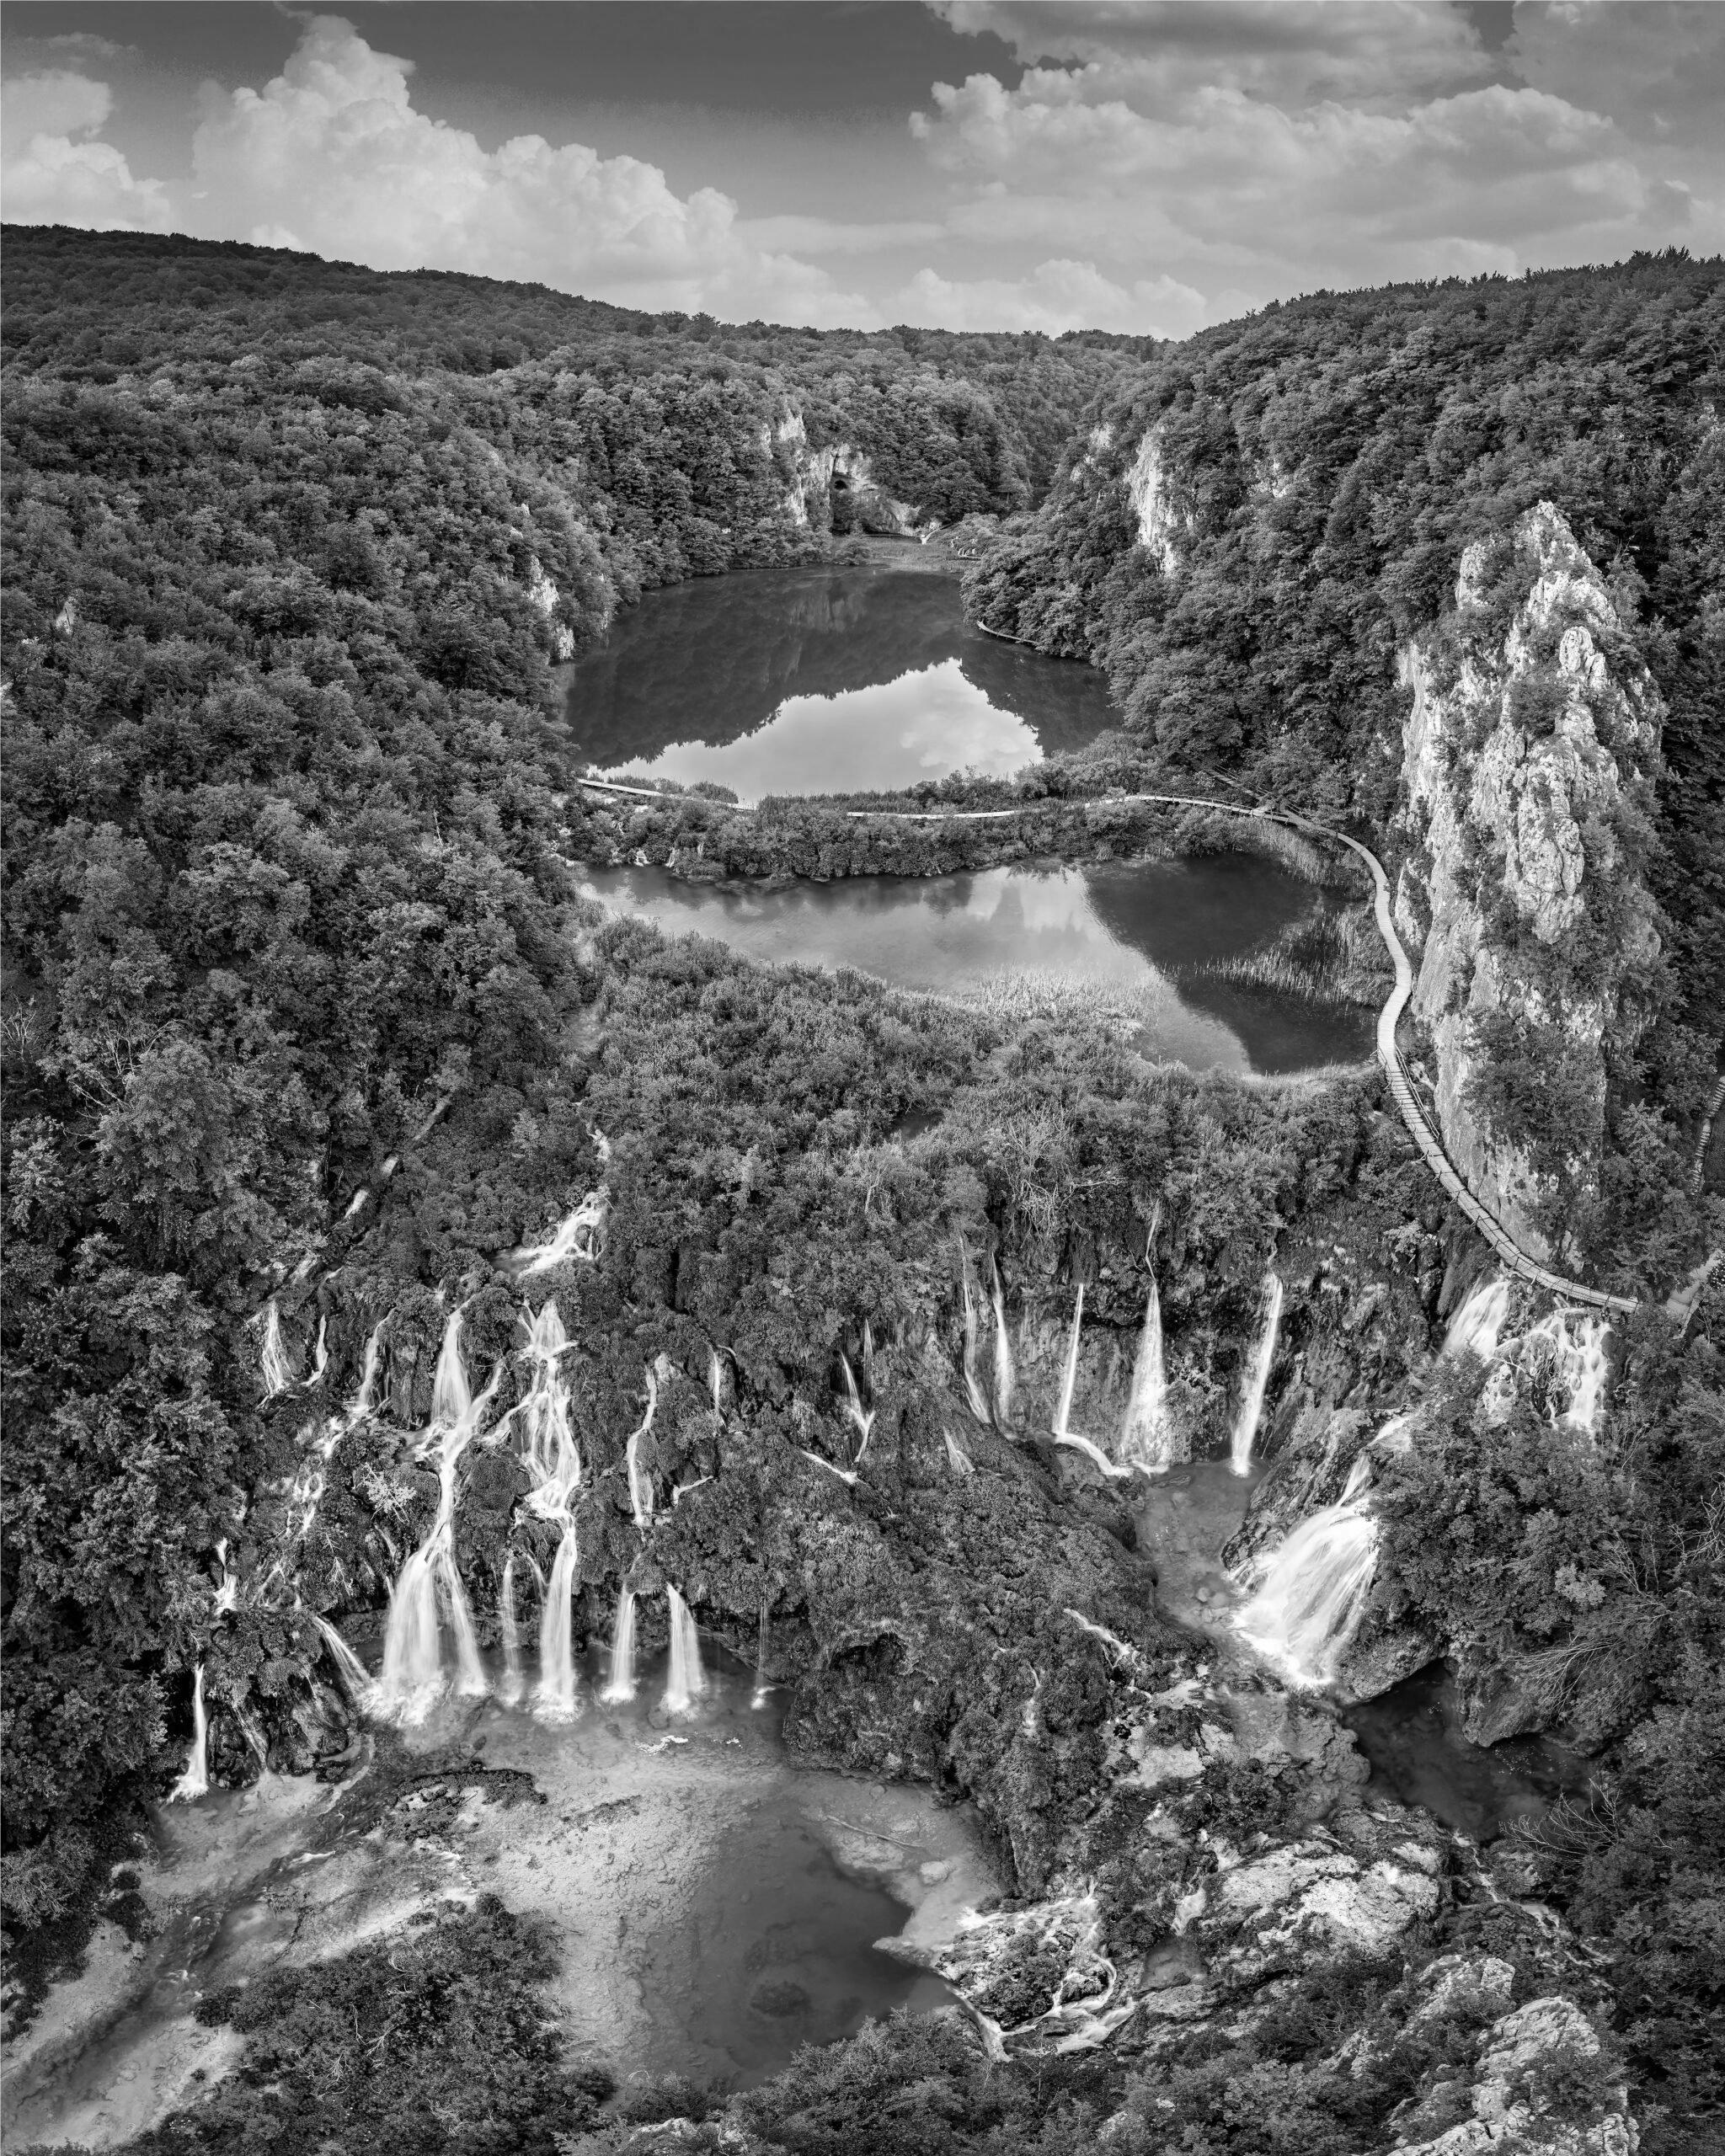
\includegraphics[width=0.7\linewidth]{slike/Grayscale.jpeg}
    \caption{Prikaz sive slike (vlastita izrada)}
\end{figure}

Na priloženoj sivoj slici se također može vidjeti da je različita od sivih slika kanala prikazanih na \hyperref[fig:channels]{slici 1}. To je zato što se kod pretvorbe slike u boji u sivu sliku uzimaju u obzir vrijednosti piksela za sva 3 kanala prema formuli:

{\large
\[
    I_{\text{siva}}(x, y) = 0.299 \cdot R(x, y) + 0.587 \cdot G(x, y) + 0.114 \cdot B(x, y)\text{\cite{Grayscale2}}
\]
}


\subsection{Binarne slike}

Osim slika u boji i sivih slika također postoje i binarne slike. Binarne slike su poseban tip slika gdje piksel može imati samo dvije moguće vrijednosti od kud im dolazi i naziv, te vrijednosti su nula ili jedan. Binarne slike sadrže puno manje informacija od ostalih tipova slika, ali isto tako smanjuju kompleksnost same slike i omogućuju fokusiranje na važne značajke slike. Baš zbog toga se jako često koriste kod obrada slika koristeći računalni vid \cite{BinarySlika}.

\begin{figure}[H]
    \centering
    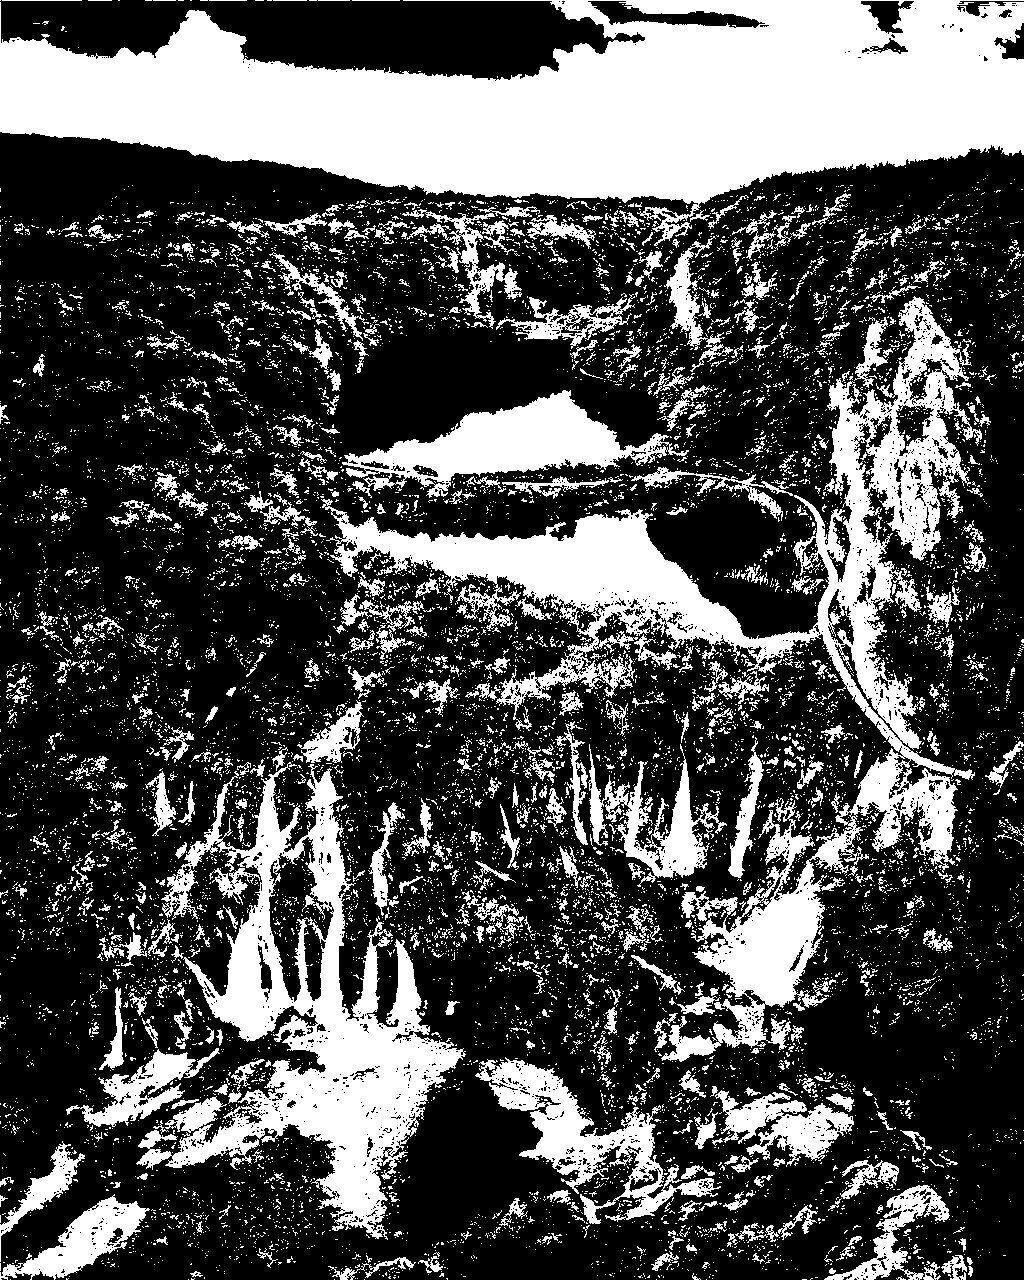
\includegraphics[width=0.75\linewidth]{slike/Binary.jpeg}
    \caption{Prikaz binarne slike (vlastita izrada)}
\end{figure}

Sam proces izrade binarne slike je dosta jednostavan. Za početak potrebno je imati sivu sliku. Zatim se definira granica (\textit{eng. threshold}) u obliku postotka ili vrijednosti piksela. Ta granica se zatim koristi za određivanje nove vrijednosti piksela, ako je vrijednost iznad granice onda se vrijednost postavlja na jedan, a inače na nulu. Priložena formula prikazuje osnovni tip kreiranja binarne slike (\textit{eng. tresholding}).

{\large
    \[
I_{\text{siva}}(x, y) = 0.299 \cdot R(x, y) + 0.587 \cdot G(x, y) + 0.114 \cdot B(x, y)
\]

\[
I_{\text{binarna}}(x, y) =
\begin{cases}
1, & \text{ako } I_{\text{siva}}(x, y) \geq T \\
0, & \text{ako } I_{\text{siva}}(x, y) < T
\end{cases}
\]}


\subsection{Važnost različitih tipova digitalnih slika}

Do sada smo prošli kroz 3 najvažnija tipa digitalnih slika za ovaj rad. Kroz ovu cjelinu prikazat će se važnost pojedinog tipa slike naspram ostalih.

Zapravo najveća razlika između ovih tipova je broj kanala boje. Slike u boji imaju 3 kanala za razliku od sivih i binarnih slika koje imaju po jedan kanal. To zapravo znači da slike u boji sadrže značajno više informacija. 

No ponekad nam te informacije nisu potrebne ovisno o problemu koji pokušavamo riješiti. Na primjer ako pokušavamo detektirati boju svjetla na semaforu onda su nam informacije o bojama izrazito važne. No ako pokušavamo pročitati tekst s prometnog znaka onda nam informacija o boji znaka i teksta ne doprinosi značajno rješavanju problema. Zapravo nam otežava rješavanje problema pošto moramo raditi s nepotrebnim informacijama.

\begin{figure}[H]
    \centering
    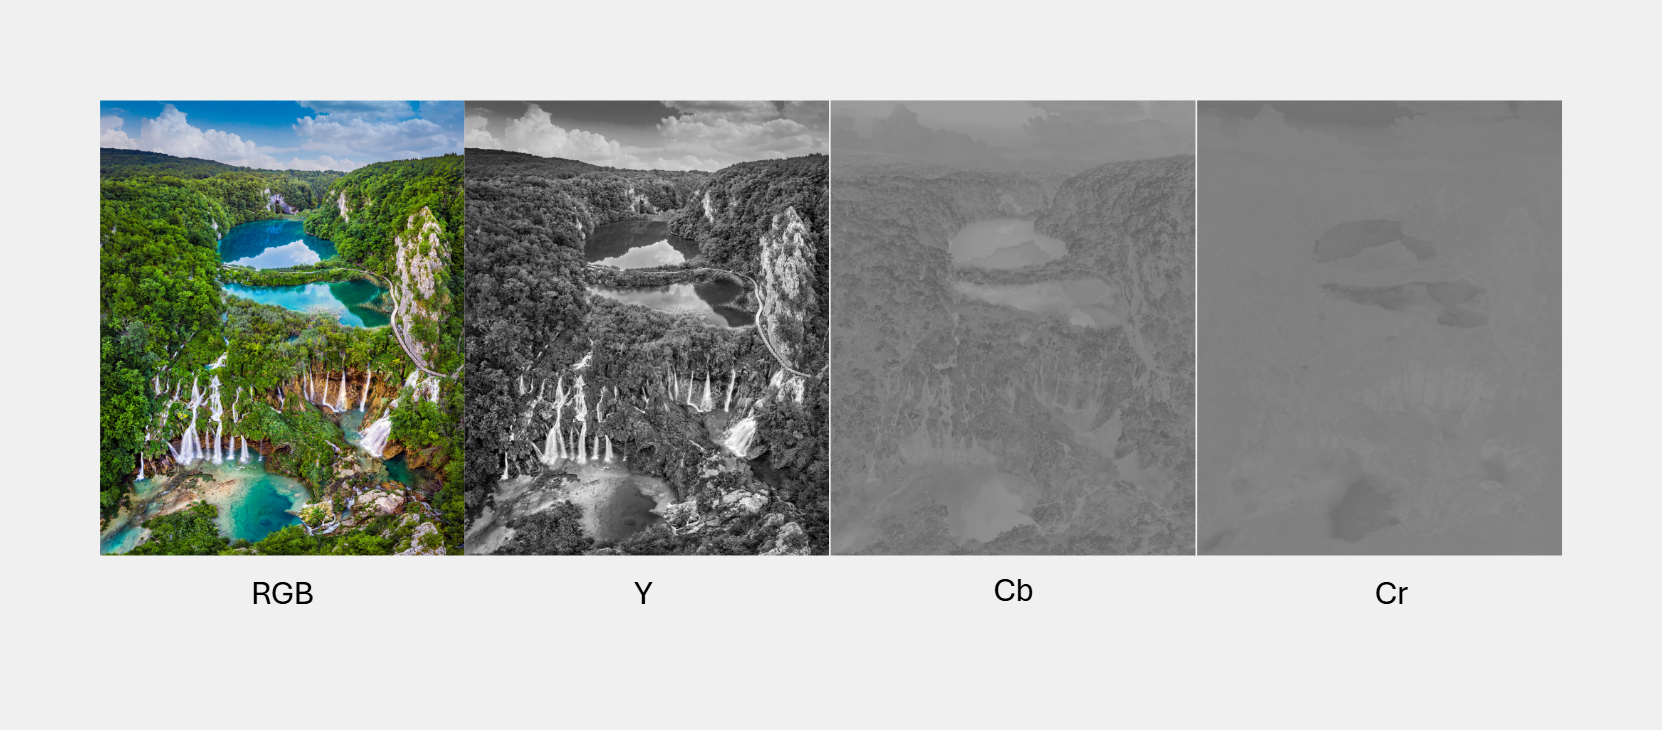
\includegraphics[width=1.0\linewidth]{slike/Luminace vs chrominance.png}
    \caption{Usporedba svjetlosne komponente i komponenta boja(vlastita izrada)}
\end{figure}

\begin{flushleft}
    Na priloženoj slici prikazana je ista slika na različite načine:
    \begin{itemize}[label=•]
        \item Slika u RGB formatu
        \item Slika u YCbCr formatu
        \begin{itemize}[label=•]
            \item Svjetlosne informacije u Y kanalu
            \item Informacije o bojama u Cb i Cr kanalima
        \end{itemize}
    \end{itemize}
    \end{flushleft}

Na ovom primjeru je prikazana činjenica da svjetlosni kanali sadrže puno više informacija o strukturnim elementima na slici. Baš zbog toga se u raznim algoritmima za detektiranje značajki, filtriranje, segmentiranje i sl. koriste baš sive slike \cite{LumVsChrom}. 

Sive slike se koriste kada boja nije važan faktor u obradi slike. U tom slučaju je boja jednako korisna kao buka na slici pa je zbog toga uklonimo. Time se veličina slike smanjuje i ujedno se ubrzava daljnji proces obrade slike \cite{LumVsChrom}.

Ako je potreban još agresivniji pristup otklanjanju nepotrebnih podataka, binarne slike mogu biti korisne. One dodatno odstranjuju nepotrebne podatke tako da povećavaju razliku u kontrastu i time odvajaju razne strukturne elemente slike \cite{LumVsChrom}.

Važno je napomenuti da svaki tip slika ima svoju upotrebu ovisno o problemu koji se rješava. U ovom radu će veliku važnost imati sive i binarne slike pošto se radi o procesu detektiranja strukture fotografije i izvlačenja relevantnih informacija iz nje.

\section{Digitalna obrada slike}

Digitalna obrada slike (\textit{eng. digital image processing}) podrazumijeva obradu digitalne fotografije koristeći računalne algoritme s ciljem unaprjeđivanja slike, izvlačenja korisnih informacija, analize, izrade izvještaja i slično. Predstavlja ključni korak u raznim primjenama računalnog vida temeljenog na dubokom učenju, poput prepoznavanja lica, detekcije objekata i optičke detekcije \cite{ImageProcessing}. 

\begin{flushleft}
Sam proces digitalne obrade slike može se podijeliti u sljedeće faze \cite{ImageProcessing}:
\begin{itemize}
\item Pribavljanje slike (\textit{eng. image acquisition})
\item Poboljšanje slike (\textit{eng. image enhancement})
\item Kompresija slike (\textit{eng. image compression})
\item Morfološka obrada (\textit{eng. morphological processing})
\item Segmentacija slike(\textit{eng. image segmentation})
\item Reprezentacija i opis (\textit{eng. representation and description})
\item Detekcija i prepoznavanje objekata (\textit{eng. object detection and recognition})
\end{itemize}
\end{flushleft}

Naravno nisu sve faze uvijek potrebne, već se radi o generalnim smjernicama koje se prema specifičnostima problema mogu modificirati, smanjiti ili proširiti. U nekim slučajevima čak se redoslijed faza može promijeniti ili se faze mogu provoditi više puta.    

Te faze se dodatno mogu podijeliti na \textbf{pretprocesiranje, procesiranje i postprocesiranje slike}. U fazu \textbf{pretprocesiranja} spadaju svi koraci koji pripremaju sliku za procesiranje, poput poboljšanja slike. Nakon pretprocesiranja slijedi \textbf{procesiranje} koje se odnosi na korištenje algoritama za detekciju i prepoznavanje objekata i transformacije. Posljednja faza uključuje korake poput pripreme rezultata za prezentaciju, vizualizaciju i daljnju analizu \cite{IamgeProcesingPhases}.

\pagebreak
\subsection{Pretprocesiranje slike}

Pretprocesiranje slike je ključan proces koji se provodi prije obrade slike. Kao ulaz prima izvornu, sirovu sliku, a kao izlaz vraća sliku u korisnijem formatu za daljnju obradu i analizu. Omogućuje da se sa slike odstrane ili istaknu područja relevantnih informacija te da se poboljša kvaliteta slike prije daljnje obrade \cite{Patel2023Oct}.

\subsubsection{Pribavljanje slike}

Pribavljanje slike je proces nastajanja digitalne slike tako da se informacije iz realnog svijeta zapišu u digitalnom obliku kojim računalo zatim može manipulirati. Slika se može pribaviti raznim uređajima poput fotoaparata, pametnog mobitela i drugih tehnologija poput skenera, rendgena. U ovom radu fokus će biti na fotografije pribavljene uređajima koji posjeduju digitalnu kameru \cite{BibEntry2025Apr}.


Da bi bilo kakvo procesiranje moglo krenuti, prvo je potrebno pribaviti sliku. Moglo bi se reći da je pribavljanje slike čak najvažniji korak u cijelom procesu obrade slike, njegov rezultat ima veliku ulogu za postizanje krajnjeg rezultata obrade i analize slike. Pribavljena slika mora biti kvalitetna da bi ostali koraci bili uspješni. Na kvalitetu slike ne utječe samo rezolucija, već osvjetljenje i kut pod kojim je slika uslikana također imaju značajnu ulogu \cite{BibEntry2025Apr}.

Razni algoritmi i koraci u pretprocesiranju mogu korigirati pribavljenu sliku, no to nikad nije zamjena za sliku dobre kvalitete. Dobra i loša slika mogu biti razlika između uspješnog i neuspješnog detektiranja elemenata na slici. Naravno u većini slučajeva sustavi za obradu slike ne mogu utjecati na kvalitetu slike koje će im korisnik poslati. Zbog toga je važno detaljno testirati sustav u različitim uvjetima i utvrditi što su njegove granice i je li potrebno podržati neki dodatni korisnički slučaj od onih postojećih.
\subsubsection{Poboljšanje slike}

Poboljšanje slike je ključan korak, cilj mu je modificirati sliku tako da ona postane korisnija za daljnju obradu. To se može postići na više načina poput otklanjanja buke, isticanja važnih značajki slike, poboljšanja oštrine i kontrasta slike.

Do sada smo spomenuli da se nepotrebne informacije na slici također mogu biti buka. Baš zbog toga pretvaranje u sivu i binarnu sliku spada pod poboljšanje slike. Oba dvije operacije uklanjaju nepotrebne informacije o bojama sa slike što omogućuje bržu i jednostavniju obradu i analizu slike. Naravno to ima smisla samo ako nam informacije o tim bojama nisu potrebne.

Osim nepotrebnih boja, bukom se može smatrati i nasumična razlika u vrijednosti između susjednih piksela. U digitalnoj fotografiji buka je praktički neizbježna i može se definirati kao nasumična varijacija signala u slici. Ta varijacija je reprezentirana različitim nijansama boja susjednih piksela. Buka se može smanjiti manipulacijom parametara digitalne kamera, ali ne može se kompletno ukloniti \cite{Adobe}.

Takve informacije se zbog malih razlika u boji piksela većinom mogu smatrati nevažnima, a loše utječu na daljnju obradu slike. Zbog toga postoje razne tehnike za filtriranje slike. Najpopularnije tehnike za filtriranje buke su \cite{Swain2023Jul}:

\begin{itemize}
    \item Gaussov filter (\textit{eng. gaussian filter})
    \item Srednji filter (\textit{eng. mean filter})
    \item Medijanski filter (\textit{eng. median filter})
    \item Bilateralni filter (\textit{eng. bilateral filter})
\end{itemize}


Svaki tip filtera ima svoju upotrebu i koristan je za određeni tip buke. Buka u digitalnim slikama je jako opširna tema koje se neće detaljnije objašnjavati u ovom radu.

\begin{figure}[H]
    \centering
    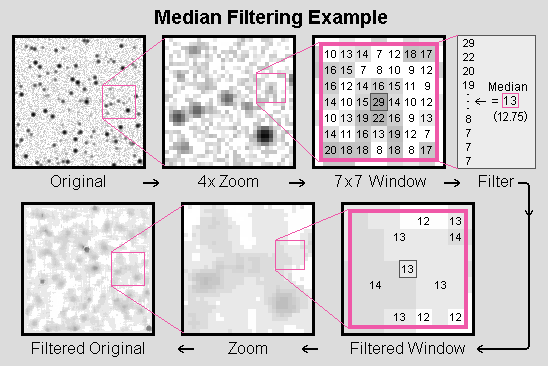
\includegraphics[width=0.85\linewidth]{slike/MedianFiltering.png}
    \caption{Primjer medijanskog filtera \cite{MeidanFilter}}
\end{figure}

Na priloženoj slici je prikazan proces korištenja medijanskog filtera koji naspram matrice susjednih vrijednosti određuje vrijednost piksela koristeći medijan svih vrijednosti.

Važno je napomenuti da su pojmovi poput oštrine i mutnoće  slike usko povezani s bukom. Jako često mutna slika sadrži manje buke, dok oštra slika može sadržavati više buke. Zbog toga je potrebno naći ravnotežu pri uklanjanju buke. Ako uklonimo previše buke, slika postaje mutna i gubi se previše informacija, obrnuto vrijedi ako uklonimo premalo buke.

Uklanjanje buke jedan je od najvažnijih koraka jer se nakon njega u daljnjim fazama ne analiziraju nepotrebne i neželjene informacije. Moglo bi se reći da je to de facto obavezan korak pretprocesiranja, budući da se izrazito često koristi.

\begin{figure}[H] 
    \centering 
    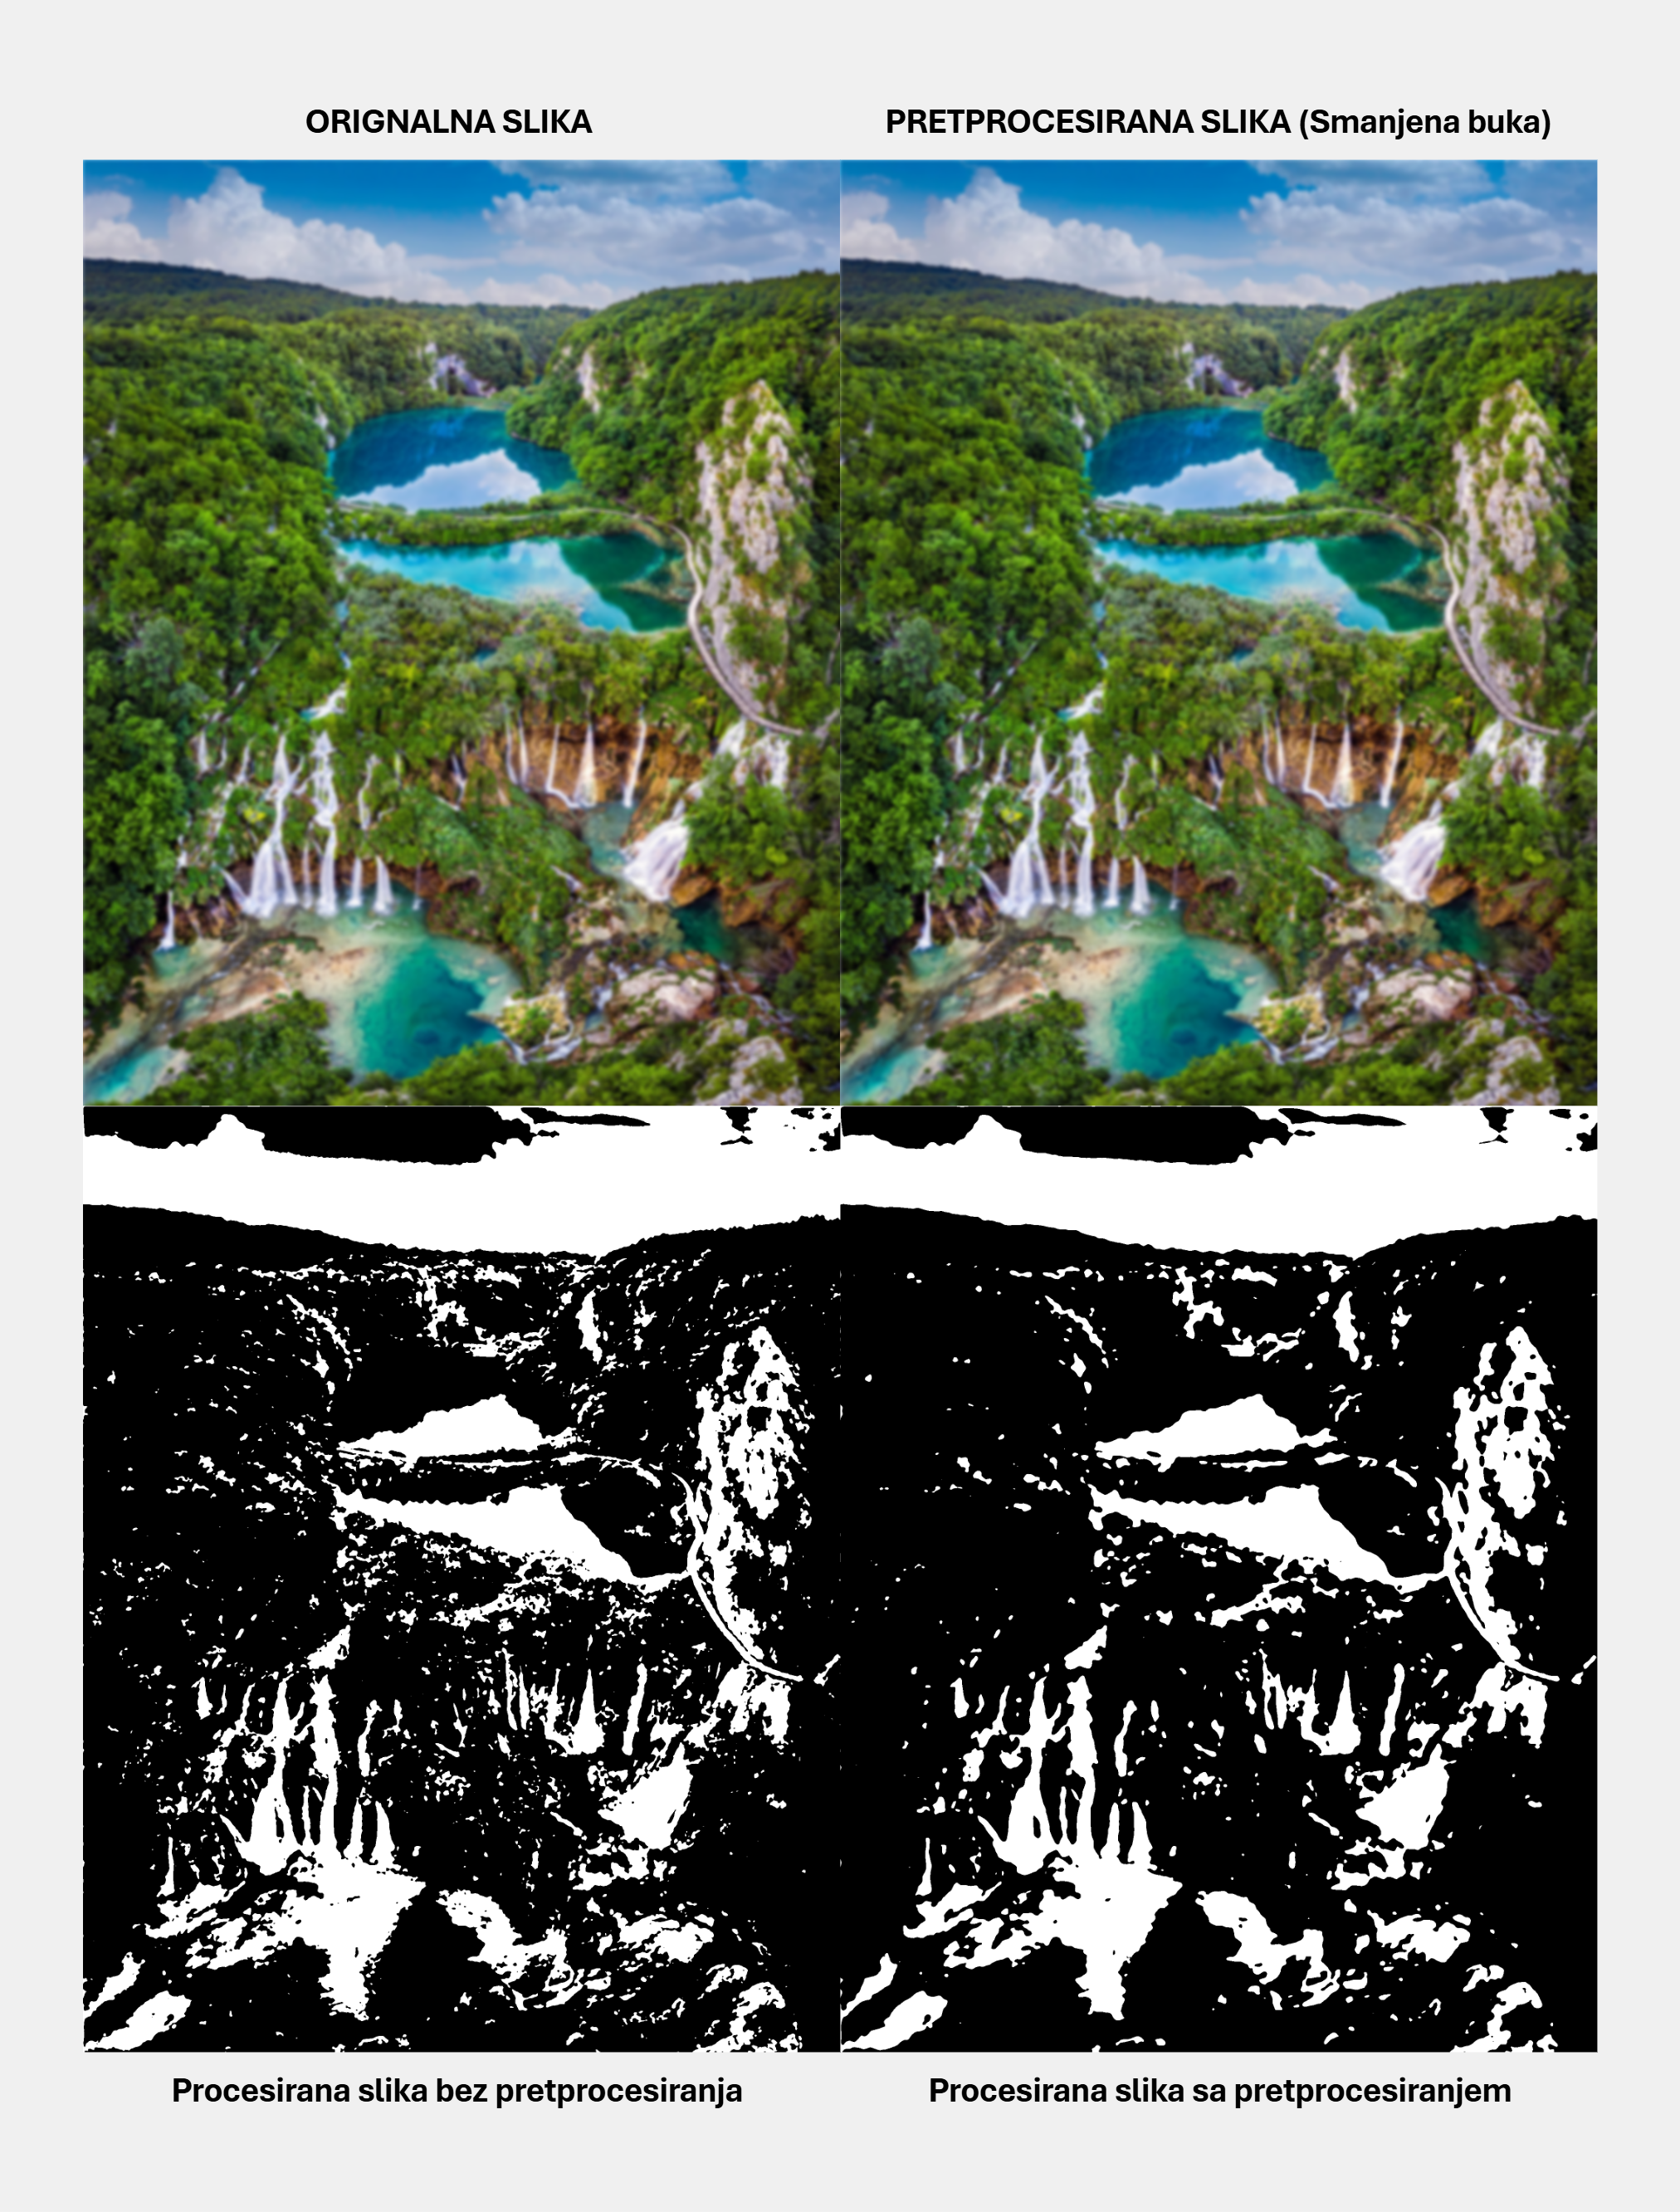
\includegraphics[width=0.85\linewidth]{slike/withAndWithoutPreProcessing.png} 
    \caption{Usporedba procesirane slike bez i s pretprocesiranjem (vlastita izrada)} 
\end{figure}

Na priloženoj slici moguće je vidjeti kako je znatno manje nevažnih informacija na desnoj binarnoj slici jer je pretprocesiranjem uklonjena buka, čime su dobiveni puno čišći podaci koji se mogu koristiti za daljnju obradu.

Postoji još razne metode poboljšavanja slike poput povećavanja kontrasta, ali neće biti potrebne u ovom radu.Također u nekim literaturama se spominju tehnike poput smanjenja buke  i raznih drugih transformacija u kontekstu restauracije slike. Ali u ovom radu će se o tome govoriti u kontekstu poboljšanja slike.

Druge važne metode poboljšavanja slike su razne geometrijske transformacije slike poput translacije, rotacije i skaliranja. Sve te osnovne geometrijske operacije koriste se kod ispravljanja perspektive. Baš zbog toga je ispravak perspektive puno zanimljivija operacija za ovaj rad \cite{GeometryTransforms}.

Ispravljanje perspektive omogućuje da slika prikazuje kao da je slikana u nekoj drugoj ravnini u prostoru. To omogućuje da se uklone neželjene značajke pribavljene slike poput kuta kamere naspram subjekta fotografije, u ovom slučaju papira s matricom odgovora. 

Korekcija perspektive mapira točku \( \mathbf{p} = [x, y, 1]^T \) u originalnoj slici (slikanoj iz nekog neželjenog kuta) \( \mathbf{p'} = [x', y', w']^T \) u sliku ispravljene perspektive s pomoću matrice \( H \) \cite{OpenCvPerpsective}.

\[
\mathbf{p'} = H \cdot \mathbf{p}
\]

Gdje \( H \) predstavlja \( 3 \times 3 \) homografsku matricu:

\[
H = 
\begin{bmatrix}
h_{11} & h_{12} & h_{13} \\
h_{21} & h_{22} & h_{23} \\
h_{31} & h_{32} & h_{33}
\end{bmatrix}
\]

Transformirane koordinate se računaju na sljedeći način:

\[
\begin{bmatrix}
x' \\
y' \\
w
\end{bmatrix}
=
\begin{bmatrix}
h_{11} & h_{12} & h_{13} \\
h_{21} & h_{22} & h_{23} \\
h_{31} & h_{32} & h_{33}
\end{bmatrix}
\cdot
\begin{bmatrix}
x \\
y \\
1
\end{bmatrix}
\]

Da bi te koordinate bile korisne potrebno ih je normalizirati s \( w \):

\[
x' = \frac{h_{11}x + h_{12}y + h_{13}}{h_{31}x + h_{32}y + h_{33}}, \quad
y' = \frac{h_{21}x + h_{22}y + h_{23}}{h_{31}x + h_{32}y + h_{33}}
\]

\begin{figure}[H]
    \centering
    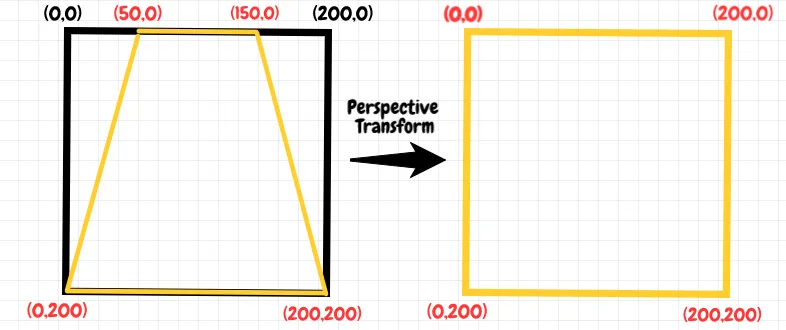
\includegraphics[width=0.85\linewidth]{slike/perspective.png}
    \caption{Prikaz procesa ispravka perspektive subjekta na slici \cite{OpenCvPerpsective}}
\end{figure}

Na priloženoj slici prikazano je kako se matrica transformacije koristi da bi se perspektiva ispravila. U praksi to funkcionira tako da se matrica transformacije računa naspram 4 izvorne i 4 odredišne točke. Te se zatim prema formuli množi sa svakom izvornom točkom da bi se izračunale odredišne točke.

\subsection{Procesiranje slike}

Nakon što je faza pretprocesiranja pretvorila sliku u korisniji format, kreće glavna faza obrade to jest procesiranje slike. Glavne tehnike kod procesiranja slike su segmentacija, detekcija objekata, morfološka obrada te reprezentacija i opis.

\subsubsection{Segmentacija slike}

Segmentacija slike je proces grupiranja piksela prema nekim obilježjima. Za razliku od običnih klasifikatora poput neuronskih mreža, segmentacija nudi informacije gdje se točno na slici nalazi objekt od interesa i koji su sve pikseli dio tog objekta. Isto kao u kod klasifikatora potrebno je definirati moguće klase kojima piksel može pripadati. Definiranje tih klasa može se učiniti na tri načina, prema kojima dijelimo tipove segmentacije na \cite{segmentacija}:

\begin{itemize}
    \item semantička segmentacija (\textit{eng. semantic segmentation })
    \item segmentacija instance (\textit{eng. instance segmentation})
    \item panoptička segmentacija (\textit{eng. panoptic segmentation})
\end{itemize}

\begin{figure}[H]
    \centering
    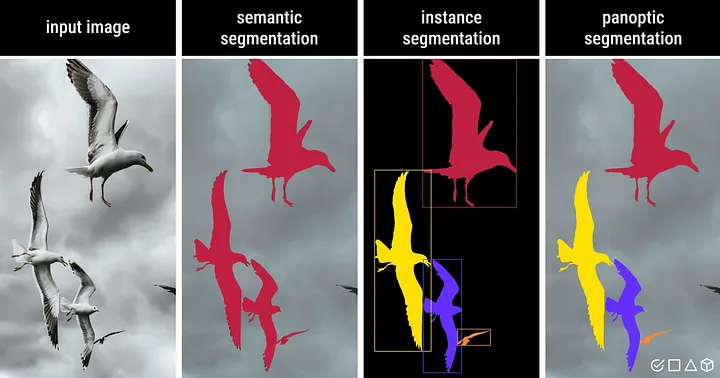
\includegraphics[width=0.85\linewidth]{slike/sesgmentacija.png}
    \caption{Usporedba tipova segmentacije \cite{segmentacija}}
\end{figure}

Na priloženoj slici definirane su dvije klase: nebo i ptice. Semantička segmentacija je sve piksele ptica klasificirala kao jednu klasu, što znači da ne znamo točno kojoj ptici pripada pojedini piksel. Da bi to riješili postoji segmentacija prema instanci što odvaja svaku pticu u zasebnu klasu što je bolje od semantičke, ali znači da više ne znamo koji sve pikseli pripadaju roditeljskoj klasi ptica. Da bi to riješili postoji panoptička segmentacija koja kombinira ta dva pristupa i pruža informacije o klasi piksela i kojoj instanci pripada. Tip segmentacije ovisi o specifičnostima problema koji se pokušava riješiti \cite{segmentacija}.


\subsubsection{Morfološka obrada}

Morfološka obrada je skup operacija koje procesiraju sliku. Omogućuje pronalazak elemenata na slici sličnih definiranom obliku. Usporedbu oblika vrši tako da traži grupu piksela koji odgovaraju tom obliku \cite{morph}.

Morfološka obrada se u nekim segmentima preklapa s segmentacijom slike, ali ne radi se o istim operacijama. Morfološke operacije se često koriste nakon segmentacije da uklone nedostatke iz detektiranih segmenata \cite{morph}.

Dvije najvažnije morfološke operacije su erozija i dilatacija.
Erozija funkcionira na način da uklanja piksele s ruba objekta. Vrlo je korisna u slučajevima kada je potrebno odvojiti dva objekta određenog oblika \cite{morph}. 

\begin{figure}[H]
    \centering
    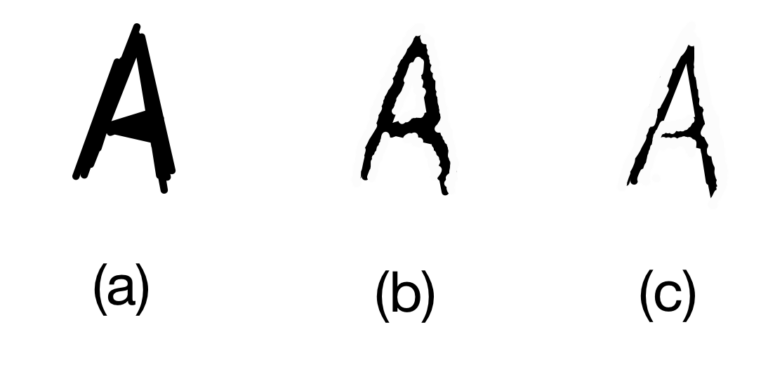
\includegraphics[width=0.75\linewidth]{slike/erosion.png}
    \caption{Prikaz erozije kao morfološke operacije \cite{morph}}
\end{figure}

Za razliku od erozije, dilatacija dodaje piksele oko ruba objekta. Time omogućuje da se popune praznine između objekata.

\begin{figure}[H]
    \centering
    
\includegraphics[width=0.75\linewidth]{slike/dilatacija.png}
    \caption{Prikaz dilatacije kao morfološke operacije \cite{morph}}
\end{figure}

Najčešće se te dvije operacije ne koriste zasebno već zajedno kao kompozitna morfološka operacija. Ako prvo provedemo eroziju, zatim dilataciju, radi se o otvaranju, dok obrnuti redoslijed operacija čini zatvaranje. \cite{morph}.

\begin{figure}[H]
    \centering
    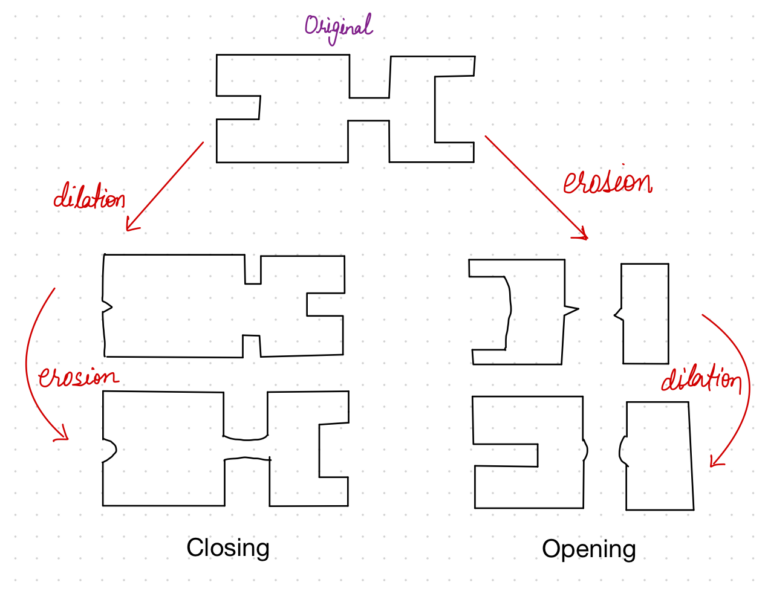
\includegraphics[width=0.6\linewidth]{slike/otvaranje_zatvaranje.png}
    \caption{Prikaz kompozitnih morfoloških operacija \cite{morph}}
\end{figure}

\subsubsection{Reprezentacija i opis}
Nakon što je obavljena segmentacija i po potrebi morfološka obrada većinom slijedi reprezentacija i opis segmentiranih dijelova. Cilj reprezentacije i opisa je reprezentirati piksele tako da budu korisniji za daljnju obradu \cite{RepAndDesc}. 

\begin{flushleft}
    Dva glavna tipa reprezentacije segmentiranih objekata, ovisno o tome je li fokus na \cite{RepAndDesc}:

\begin{itemize}
    \item vanjskim karakteristikama, (kontura ili rub objekta))
    \item unutarnjim karakteristikama (pikseli koji čine objekt)
\end{itemize}
\end{flushleft}

Reprezentacija prema vanjskim karakteristikama se često koristi kad nam je za obradu važan sam oblik, dok se unutarnje karakteristike koriste kada je potrebna informacija o boji i teksturi objekta. Iz dobivenih reprezentacija je moguće izvući razne opisne vrijednosti (\textit{eng. descriptors}) koje su korisne kod daljnje obrade. Važno je napomenuti da je generalno pravilo da bi opisne vrijednosti trebale biti imune na promjenu skaliranja, translacije i rotacije \cite{RepAndDesc}.

\begin{flushleft}
Neke od korisnik opisnih vrijednosti su \cite{RepAndDesc}:
\begin{itemize}
    \item Dužina konture objekta
    \item Promjer konture objekta
    \item Zaobljenost
    \item Okvirna kutija
    \item Površina objekta
    \item Sličnost željenom obliku
    \item Odstupanje od simetrije
    \item Koeficijent istezanja
\end{itemize}
\end{flushleft}

\subsubsection{Detekcija i prepoznavanje objekata}

Detekcija i prepoznavanje objekata je jedna od ključnih tehnika procesiranja slika na tradicionalan način, ali i s pomoću neuronskih mreža. Bazirano je na principu pronalaska objekta i crtanja okvirne kutije oko tog objekta \cite{segvsdetection, , segvsdetection_2}. 

To mu je ujedno i glavna razlika naspram segmentacije slike, segmentacija dodjeljuje klasu svakom pikselu koji odgovara onome što se traži, dok detekcija objekta to ne radi već samo locira objekt određene klase na slici \cite{segvsdetection, segvsdetection_2}.

Ponekad je samo informacija o lokaciji objekta dovoljna, u slučaju da nije segmentacija nudi puno više informacija o samom objektu.

Da bi detektiranje objekata bilo uspješno često se koriste konture. Konture su ništa drugo nego krivulje koje opisuju rubove objekata, zbog toga su jako korisne kod detektiranja oblika. Također se ponekad koriste i kod segmentiranja.

\begin{figure}[H]
    \centering
    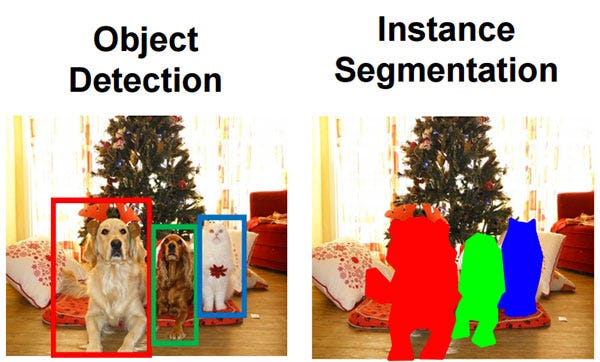
\includegraphics[width=0.6\linewidth]{slike/segVsDetec.png}
    \caption{Usporedba segmentacije i detekcije objekta \cite{segvsdetection_2}}
\end{figure}

Da bi se mogle pronaći konture prvo je potrebno sliku pretvoriti u binarnu sliku i zatim provesti operaciju detektiranja kontura. Konture se detektiraju tako da se traži razlika između kontrasta piksela na binarnoj slici i time se utvrđuje ujedno i granica između objekata. Zatim se primjenjuje jedna od metoda za detekciju objekta nad tim konturama. Te metode zapravo traže konture koje odgovaraju traženom obliku s definiranim tolerancijama za oblik, veličinu i slično \cite{konturesShapes}.

\begin{flushleft}
Budući da se u ovom radu koristi pristup temeljen na tradicionalnoj obradi slike, od posebnog su interesa sljedeće metode koje omogućuju detekciju i analizu geometrijskih oblika koristeći konture:

\begin{itemize}
\item \textbf{Aproksimacija kontura u poligone} - koristi se za pojednostavljenje kontura i prepoznavanje osnovnih geometrijskih oblika.
\item \textbf{Izračun minimalnog pravokutnika oko konture} - omogućuje određivanje najmanjeg pravokutnika koji obuhvaća određeni objekt, što je korisno pri detekciji pravokutnih oblika.
\item \textbf{Prilagodba elipse konturi} - koristi se za identifikaciju objekata eliptičnog oblika.
\item \textbf{Detekcija ravnih linija Houghovom transformacijom} - omogućuje otkrivanje linijskih struktura unutar slike.
\item \textbf{Detekcija kružnica Houghovom transformacijom} - primjenjuje se za prepoznavanje kružnih objekata.
\item \textbf{Pronalaženje pravokutnog okvira oko konture (bounding box)} - omogućuje okvirno lociranje objekta unutar slike.
\item \textbf{Detekcija kontura s hijerarhijskim odnosima} - omogućuje razlikovanje vanjskih i unutarnjih kontura, što je korisno pri analizi složenijih objekata.
\end{itemize}
\end{flushleft}

\begin{figure}[H]
    \centering
    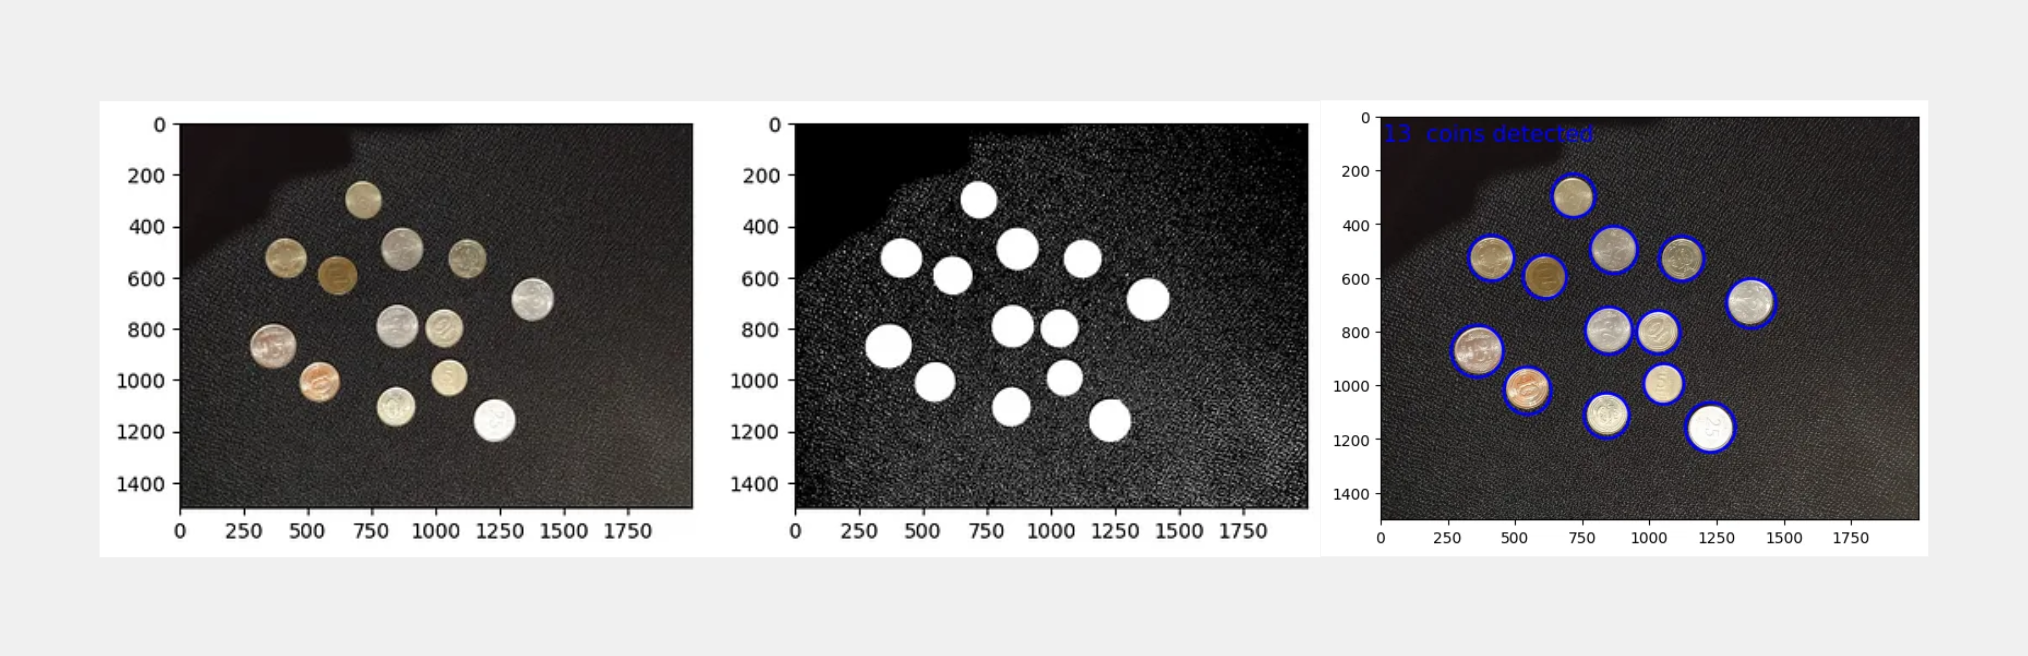
\includegraphics[width=1.0\linewidth]{slike/shapeDetection.png}
    \caption{\centering Prikaz rezultata detekcije krugova pomoću kontura \cite{segvsdetection_2}}
\end{figure}

Na priloženoj slici je jasno prikazano kako se izvorna slika pretvara u binarnu sliku i zatim se s pomoću kontura i metode za detektiranje oblika naspram kontura pronalazi lokacija kruga.

\subsection{Postprocesiranje slike}

Nakon što je glavna faza obrade slike završena kreću aktivnosti postprocesiranja. Prijašnja faza je izvukla korisne podatke iz slike i pripremila ih u korisnom formatu. Cilj postprocesiranje je obrada tih podataka tako da se dođe do konačnog rješenja. Osim obrade podataka, postprocesiranje je također povezano s aktivnostima poput vizualizacije rezultata, kompresije i slično.

\subsubsection{Obrada izvučenih podataka}

\begin{flushleft}
    Prije nego što se krene u konačnu obradu izvučenih podataka potrebno ih je pročistiti. Načini pročišćavanja podataka ovise o specifičnostima problema, ali neke od važnih metoda za ovaj rad su:
\begin{itemize}
    \item Filtriranje po veličini objekta
    \item Filtriranje po obliku objekta
    \item Filtriranje po boji objekta
    \item Filtriranje po hijerarhijskoj odnosu objekta s ostalim objektima
\end{itemize}
\end{flushleft}

Spomenute metode bazirane su na usporedbi opisnih vrijednosti iz faze reprezentacije i opisa. Nakon što su podaci pročišćeni kreće konačna faza obrade. Način konačne obrade ovisi o specifičnostima problema, ali često se koriste baze znanja.

Baze znanja omogućuju usporedbu traženih podataka s pročišćenim podacima koje omogućuje rješenje specifičnog problema. U ovom slučaju baza znanja bi bila lista odgovora za svako pitanje podijeljenih u dvije klase koje predstavljaju točne i netočne odgovore \cite{ImageProcessing}. 

\subsubsection{Vizualizacija rezultata}

Nakon što su podaci obrađeni i utvrđen je rezultat jako često ga je potrebno vizualizirati. Vizualizacija nudi uvid u njihovu važnost i omogućuje da se jednostavnije analiziraju i izvode zaključci iz rezultata. 
Tip vizualizacije ovisi o domeni problema koji se rješava. Može biti u raznim oblicima poput PDF izvješća, vizualizacije rezultata nad originalnom slikom i slično  \cite{Visulization}.

Kod vizualiziranja rezultata važno je uzeti u obzir tip podataka koji se vizualizira, publiku za koju je vizualizacija namijenjena \cite{Visulization}. 

\subsubsection{Kompresija slike}

U slučaju potrebe za smanjenjem veličine slike, često se koristi kompresija. Kompresija nastoji smanjiti veličinu slike na način da pritom zadrži kvalitetu na zadovoljavajućoj razini. Često se primjenjuje kada je potrebno smanjiti veličinu slike pri prijenosu preko mreže, spremanju u memoriju ili za ubrzanje obrade \cite{ImageProcessing}.

\begin{flushleft}
Kompresija slike dijeli se na dva glavna tipa \cite{Compression}:
\begin{itemize}
    \item Kompresija s gubitkom podataka (\textit{eng. lossy})
    \item Kompresija bez gubitka podataka (\textit{eng. lossless})
\end{itemize}
\end{flushleft}

Oba tipa smanjuju veličinu slike, ali se razlikuju u načinu na koji to postižu.  
Prvi pristup uklanja određene informacije iz slike kako bi smanjio njezinu veličinu (lossy), dok drugi pristup efikasnije zapisuje podatke bez gubitka informacija (lossless).  
Važno je napomenuti da je kod kompresije uvijek potrebno balansirati veličinu slike i kvalitetu. Što je slika više komprimirana, to je izraženija distorzija slike.  
Glavna razlika između ovih dvaju pristupa je u tome može li se originalna slika potpuno rekonstruirati iz komprimirane slike \cite{Compression}.

\pagebreak


\section{Analiza postojećih rješenja i pristupa problemu}

Prije praktičnog dijela rada važno je analizirati postojeća rješenja na tržištu. Ova analiza fokusirat će se samo na detekciju odgovora na pismenim ispitima koristeći matricu odgovora to jest detekciju OMR tehnikom (\textit{eng. optical mark recognition}). Pod OMR spadaju sve tehnike koje su do sada obrađene. Fokus ove analize je samo na rješenjima visoke razine točnosti.

Osim korištenja računalnog vida uz OMR sve češći su pristupi koji koriste elemente dubokog učenja, samostalno ili u kombinaciji s tradicionalnim računalnim vidom \cite{OMRComparsion}.

Analizirana su rješenja OMRChecker i OpenMCR, radi se o rješenjima izrazito visoke točnosti koji tu točnost zadržavaju i kada je slika uslikana u izrazito izazovnim uvjetima. Također oba rješenja podržavaju određeni stupanj konfiguracije liste s odgovorima \cite{OMRComparsion}.

\begin{figure}[H]
    \centering
    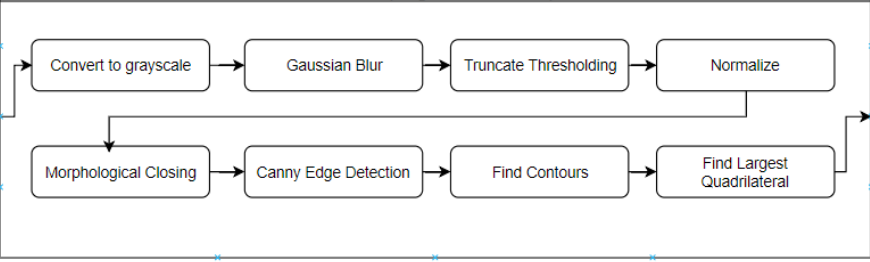
\includegraphics[width=1.0\linewidth]{slike/omr_flow.png}
    \caption{Prikaz dijela toka procesiranja slike kod OMRChecker-a \cite{OMRChecker}}
\end{figure}

S priložene slike vidljivo je da OMRChecker koristi veliku večinu metoda i tehnika koje su do sada obrađene u ovom radu, za OpenOMR je sitaucije također dosta slična.

Osim samih značajki sustava važno je znati kako su se ti sustavi nosili sa problemima pri detekciji odgovora spomenutih u prijašnjim poglavljima. Jedan od glavnih problema je kvaliteta pribavljene fotografije. To uključuje loše uvjete osvjetljenja, udaljenost uređaja od papira, kut snimanja i slične čimbenike.

Rješenja poput OpenMCR riješila su problem kuta snimanja i rotacije papira tako da su na matricu odgovora postavljena posebne oznake pomoću kojih se precizno detektiraju kutovi matrice i određuje orijentacija papira.

Na priloženoj slici prikazana su te posebne oznake koja olakšavaju detekciju kutova papira. Na lijevoj slici prikazana je matrica odgovora OMRChecker sustava, koja koristi četiri identične oznake za detekciju kutova papira. Na desnoj slici prikazana je matrica odgovora OpenMCR sustava, koja koristi tri identične oznake i jednu unikatnu. Ta različita oznaka omogućuje ne samo detekciju kutova, već i određivanje orijentacije papira.

To znači da OpenMCR nudi kvalitetnije rješenje barem što se tiće korekcije kuta snimanja i rotacije papira u odnosu na OMRChecker.

\begin{figure}[H]
    \centering
    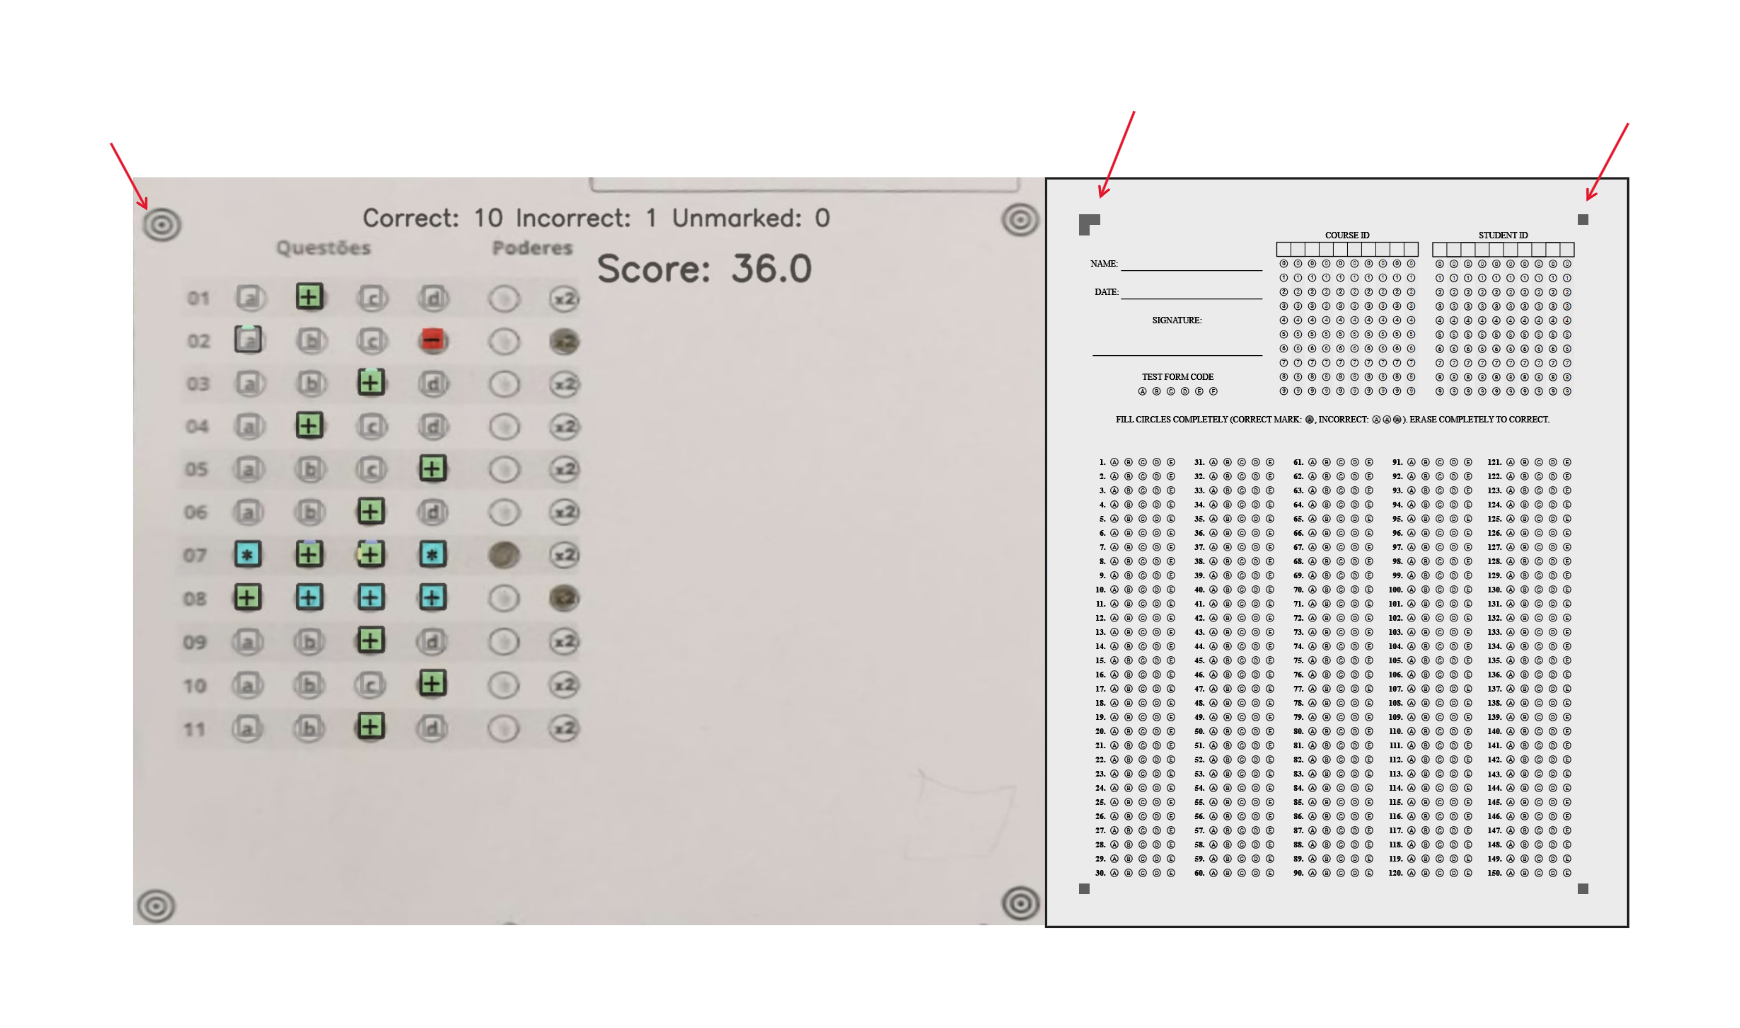
\includegraphics[width=0.9\linewidth]{slike/CornerDetection.png}
    \caption{Prikaz pomoćnih oznaka za detektiranje kutova matrice odgovora i orijentacije \cite{OMRChecker} \cite{OpenMCr}}
\end{figure}

Osim problema s kvalitetom pribavljene slike, postoje i problemi s neispravnim označavanjem područja za odgovor. Taj je problem teško riješiti korištenjem tradicionalne obrade slike, te stoga ima više smisla koristiti strojno učenje, odnosno određeni tip klasifikatora \cite{omrnet}.

OMRNet je jedno od takvih rješenja. Ono nudi mogućnost klasifikacije područja odgovora kao označeno, neoznačeno i prekriženo. Zapravo se ne radi o cjelovitom sustavu za ocjenjivanje ispita, već o sustavu koji pruža REST API za klasifikaciju područja odgovora, te se može integrirati s drugim sustavima za detekciju odgovora i ocjenjivanje ispita \cite{omrnet}.

\begin{figure}[H]
    \centering
    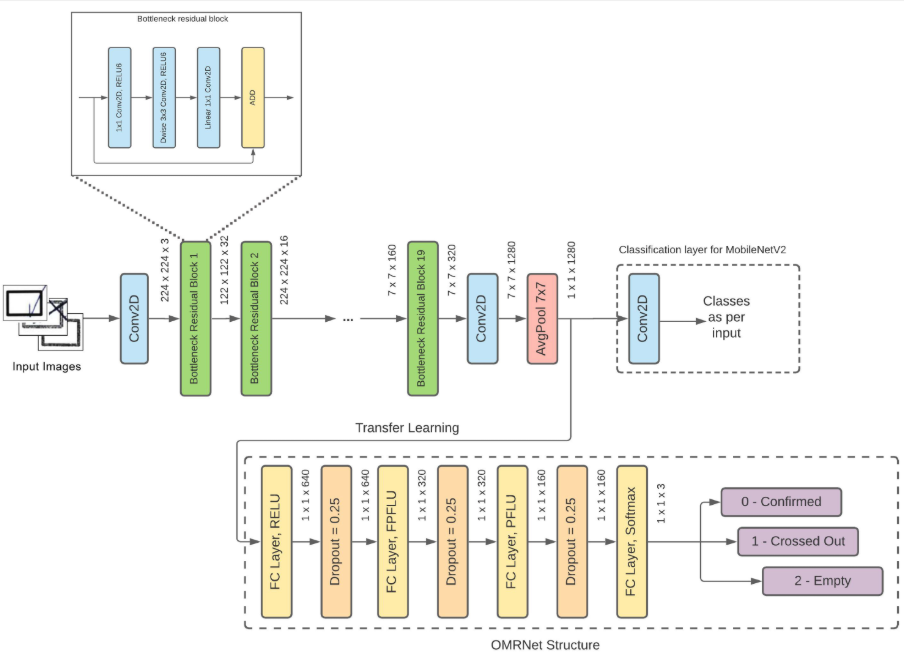
\includegraphics[width=0.7\linewidth]{slike/OMRNet.png}
    \caption{Prikaz strukture OMRNet klasifikatora \cite{omrnet}}
\end{figure}

Također, važno je napomenuti da ova konvolucijska neuronska mreža koristi metodu prijenosa znanja (eng. transfer learning) s već prethodno treniranog modela MobileNet V2 \cite{omrnet}.

Cijela svrha korištenja OMRNet-a ili neke druge implementacije dubokog učenja za klasifikaciju područja odgovora jest rješavanje problema koje OMR sustavi temeljeni isključivo na tradicionalnoj obradi slike imaju \cite{omrnet}:

\begin{flushleft}
\begin{itemize}
\item Teško je razaznati radi li se o prekriženom odgovoru ili o označenom odgovoru
\item Problem definiranja praga koji određuje je li odgovor označen ili nije
\end{itemize}
\end{flushleft}

Važno je napomenuti da su sva analizirana rješenja u određenoj mjeri ograničena kada je riječ o fleksibilnosti predloška matrice odgovora. Naime, postojeća rješenja očekuju da se na papiru nalaze određene strukture, poput oznaka za kutove i orijentaciju, specifičan broj pitanja i odgovora i slično. Sama fleksibilnost rješenja ovisi o tome je li sustav dizajniran da strogo slijedi zadani predložak ili je već u samom dizajnu predviđena određena razina prilagodljivosti.

Također, sva rješenja variraju u razini pouzdanosti i konzistentnosti u ekstremnim uvjetima rada. Pod time se podrazumijevaju visoka razina šuma, loši uvjeti osvjetljenja, ekstremni kutovi fotografiranja i slično. Međutim, postavlja se pitanje je li uopće nužno da sustav pouzdano funkcionira u takvim ekstremnim uvjetima. Na primjer nije jednaka razina pouzdanosti potrebna sustavu za ocjenjivanje ispita i sustavu za čitanje registarskih tablica na parkiralištu. Glavni razlog za to je činjenica da ocjenjivač može u velikoj mjeri kontrolirati uvjete i način pribavljanja fotografije, dok na parkiralištu to najčešće nije moguće.

Osim navedenih ograničenja, analizirana rješenja imaju i niz prednosti. Sva rješenja postižu izrazito visoku razinu točnosti koja je otprilike 99,5\%. Važno je istaknuti da za postizanje te razine preciznosti nisu potrebni značajni računalni ni vremenski resursi. Takvi sutavi također značajno skraćuju sam proces ocjenjivanja ispita u usporedbi s čovjekom. Iako ovi sustavi nisu savršeni, riječ je o zreloj i relativno jeftinoj tehnologiji koja pokazuje znatno nižu stopu pogrešaka u odnosu na čovjeka, pogotovo kada se uzme u obzir vrijeme potrebno za ocjenjivanje.

Za kraj, važno je napomenuti da je takve sustave teško međusobno uspoređivati, budući da se implementacije često razlikuju samo po korištenim metodama, dok su same faze obrade u većini slučajeva jednake i već su obrađene u prijašnjim poglavljima. Dobar primjer toga je otklanjanje šuma, koje je praktički neizostavan korak u svim sustavima, razlika je jedino u konkretnoj metodi koja se koristi za tu svrhu.

Ipak, postoje i inovativna rješenja koja pristupaju postojećim problemima na kreativan način. Dobar primjer za to je OMRNet klasifikator, koji primjenom metode dubokog učenja nudi novu perspektivu u detekciji označenih odgovora. Kombinacijom različitih aspekata postojećih rješenja moguće je dizajnirati kvalitetan i precizan sustav za detekciju i ocjenjivanje pismenih ispita zatvorenog tipa.

\chapter{Definiranje zahtjeva}

Kroz daljnji dio rada fokus će biti na izradi i prikazu komponente otvorenog koda za detekciju odgovora na pismenim testovima. Prikazat će se svi važni koraci i dizajnerske odluke koje utječu na konačni dizajn i funkcionalnost rješenja. Izrađena komponenta će također biti ugrađena u jednostavnu stolnu aplikaciju da bi se olakšalo razvoj i vizualizirao sam rad komponente. 

\section{Opis rješenja}

Kao što je već spomenuto cilj je izraditi komponentu otvorenog koda za detekciju odgovora na pismenim ispitima. Fokus će biti na detektiranju odgovora s matrice odgovora. Prednost toga pristupa je to što nije potrebno slikati više stranica da bi se ocijenio jedan ispit, već je dovoljno ocijeniti samo matricu odgovora, to jest obraditi samo jednu stranicu. 

Taj pristup detekciji odgovora je puno jednostavniji problem za riješavanje nego detekcija na standardnim ispitima. Jednostavniji je zbog toga što matrica može imati unaprijed definiranu i standardiziranu strukturu to jest predložak. Unatoč tome matrica limitira rješenje samo na pitanja s višestrukim ili jednostrukim odgovorima. No to nije problem za ovaj rad pošto drugi tipovi pitanja nisu u opsegu ovog rada.

Jedan od glavnih ciljeva ovog rješenja je da konzistentno pruža pouzdane rezultate, čak i ako uvjeti u kojima je slika uslika nisu idealni. Ta pouzdanost se treba postići za predloške koji mogu sadržavati varijabilan broj pitanja i odgovora. Da bi izrada predložaka bila što jednostavnija, rješenje bi također trebalo biti sposobno prema određenim parametrima generirati predložak matrice odgovora u obliku PDF-a. 

Također da bi se ubrzao rad s aplikacijom ideja je da korisnik ne unosi ručno podatke o točnim odgovorima za sva pitanja, već jednostavno slika ispravno riješen ispit te da komponenta sama izvuče te informacije iz fotografije. Da bi se dodatno ubrzao proces ocjenjivanja sustav treba biti dizajniran na način da detektirane odgovore usporedi s ispravnim odgovorima i ujedno prema korisnički definiranoj skali ocijeni ispit. Ocijenjeni ispit mora biti vizualiziran kako bi ocjenjivač mogao uvidjeti je li došlo do greške kod ocjenjivanja.

U svrhu bržeg razvoja, pronalaska grešaka i slično sustav bi trebao imati mogućnost vizualiziranja svakog koraka obrade od samog unosa slike pa sve do rješenja. Ta opcija bi se trebala moći uključiti ili isključiti po potrebi. 

Budući da se radi o komponenti otvorenog koda želja je da se ostavi mogućnost zamjene važnih biblioteka koje će sustav koristiti, poput one za računalni vid. Time će se omogućiti da netko po potrebi napiše svoju implementaciju i zamijeni zadanu EmguCv biblioteku.

\pagebreak

\section{Funkcionalni zahtjevi}


\begin{longtable}{|l|p{12cm}|}
    \hline
    \textbf{Identifikator} & FZ-01 \\ \hline
    \textbf{Zahtjev} & Sustav mora detektirati odgovore s matrice odgovora. \\ \hline
    \textbf{Opis} & Detekcija se temelji isključivo na obradi jedne stranice to jest matrice odgovora. Odgovori se trebaju detektirati, klasificirati prema tome jesu li označeni i zatim ih pridužiti odgovarajućem pitanju.\\ \hline
    \textbf{Način provjere} & Prilikom unosa slike matrice odgovora, sustav treba pravilno označiti sve odgovore na slici i označitiji ih odgovarajučom bojom ovisno o klasi kojoj pripadaju. \\ \hline
    \textbf{Prioritet [1--5]} & 5 \\ \hline
    \multicolumn{2}{|c|}{} \\ \hline
    
    \textbf{Identifikator} & FZ-02 \\ \hline
    \textbf{Zahtjev} & Sustav mora omogućiti generiranje PDF predložaka za matricu odgovora. \\ \hline
    \textbf{Opis} & Korisnici trebaju moći jednostavno izraditi matricu s unaprijed definiranim brojem pitanja i odgovora. \\ \hline
    \textbf{Način provjere} & Iz sustava treba biti moguće izvesti generirani predložak u PDF formatu, parametri za unos su broj pirtanja i broj odgovora po pitanju. \\ \hline
    \textbf{Prioritet [1--5]} & 3 \\ \hline
    \multicolumn{2}{|c|}{} \\ \hline
    
    \textbf{Identifikator} & FZ-03 \\ \hline
    \textbf{Zahtjev} & Sustav mora omogućiti automatsko prepoznavanje točnih odgovora iz slike ispravno riješenog ispita. \\ \hline
    \textbf{Opis} & Korisnik ne mora ručno unositi odgovore; slika ispravnog rješenja bit će dovoljna za generiranje ključa. \\ \hline
    \textbf{Način provjere} & Učitavanjem slike ispravno riješenog ispita sustav mora automatski prepoznati sve točne odgovore. \\ \hline
    \textbf{Prioritet [1--5]} & 4 \\ \hline
    \multicolumn{2}{|c|}{} \\ \hline
    
    \textbf{Identifikator} & FZ-04 \\ \hline
    \textbf{Zahtjev} & Sustav mora usporediti odgovore s točnim rješenjem i izračunati ocjenu prema skali koju je korisnik definirao. \\ \hline
    \textbf{Opis} & Automatsko ocjenjivanje ubrzava proces ispravljanja i smanjuje mogućnost pogreške. \\ \hline
    \textbf{Način provjere} & Nakon što se ispiti obrade, mora biti prikazana ocjena za svaki ispit u skladu sa skalom. \\ \hline
    \textbf{Prioritet [1--5]} & 4 \\ \hline
    \multicolumn{2}{|c|}{} \\ \hline
    \pagebreak
    \hline

    \textbf{Identifikator} & FZ-05 \\ \hline
    \textbf{Zahtjev} & Sustav mora omogućiti vizualizaciju rezultata ocjenjivanja za svakog korisnika. \\ \hline
    \textbf{Opis} & Omogućava ljudsku kontrolu rezultata i ispravnost prepoznavanja i ocjenjivanja. \\ \hline
    \textbf{Način provjere} & Vizualna prezentacija ispita s označenim točnim i netočnim odgovorima mora biti dostupna. \\ \hline
    \textbf{Prioritet [1--5]} & 3 \\ \hline
    \multicolumn{2}{|c|}{} \\ \hline
    
    \textbf{Identifikator} & FZ-06 \\ \hline
    \textbf{Zahtjev} & Sustav mora omogućiti prikaz svih koraka obrade slike. \\ \hline
    \textbf{Opis} & Korisnicima i developerima ova funkcionalnost je korisna za praćenje grešaka i ponašanja sustava. Slike se trebaju prikazati tijekom obrade i spremiti na disk računala. \\ \hline
    \textbf{Način provjere} & Funkcionalnost prikazuje korake i sprema ih na disk ako je uključena, inače ne. \\ \hline
    \textbf{Prioritet [1--5]} & 5  \\ \hline
    \multicolumn{2}{|c|}{} \\ \hline
    \textbf{Identifikator} & FZ-07 \\ \hline
    \textbf{Zahtjev} & Sustav mora podržavati pitanja s jednostrukim i višestrukim odgovorima. \\ \hline
    \textbf{Opis} & Korisnici trebaju imati mogućnost definiranja pitanja koja imaju jedan točan odgovor (jednostruki izbor) ili više točnih odgovora (višestruki izbor). Sustav mora pravilno detektirati i ocijeniti oba tipa pitanja. \\ \hline
    \textbf{Način provjere} & Prilikom testiranja, sustav mora ispravno ocijeniti ispite koji sadrže oba tipa pitanja. \\ \hline
    \textbf{Prioritet [1--5]} & 4 \\ \hline
    \caption{Funkcionalni zahtjevi}
\end{longtable}

\section{Nefunkcionalni zahtjevi}

\begin{longtable}{|l|p{12cm}|}
    \hline
    \textbf{Identifikator} & NFZ-01 \\ \hline
    \textbf{Zahtjev} & Sustav mora pružati pouzdane rezultate čak i u slučaju loših uvjeta pri snimanju (npr. sjenke, loš kontrast, zakrenutost). \\ \hline
    \textbf{Opis} & U praksi slike ispita neće uvijek biti idealne kvalitete, sustav mora biti sposoban obraditi sliku i u takvim uvjetima. \\ \hline
    \textbf{Način provjere} & Sustav se testira na uzorku slika s različitim uvjetima osvjetljenja, orijentacije i kvalitete. \\ \hline
    \textbf{Prioritet [1--5]} & 3 \\ \hline
    \pagebreak
    
    \hline
    \textbf{Identifikator} & NFZ-02 \\ \hline
    \textbf{Zahtjev} & Sustav mora omogućiti jednostavnu zamjenu vanjskih biblioteka poput one za računalni vid. \\ \hline
    \textbf{Opis} & Komponenta pruža sučelje koje korisnici mogu naslijediti i napisati svoju implementaciju i time zamijeniti biblioteku za CV. \\ \hline
    \textbf{Prioritet [1--5]} & 2 \\ \hline
    \multicolumn{2}{|c|}{} \\ \hline


    \textbf{Identifikator} & NFZ-03  \\ \hline
    \textbf{Zahtjev} & Sustav mora moći detektirati odgovore na predlošku s varijabilnim brojem pitanja i odgovora \\ \hline
    \textbf{Opis} & Korisnici će moći generirati predložak s različitim brojem pitanja i odgovora, sustav ih treba sve ispravno detektirati. \\ \hline
    \textbf{Način provjere} & Testirati s raznim kombinacijama matrica odgovora sposobnost detekcije kada broj pitanja i odgovora nije fiksan, već varijabilan. \\ \hline
    \textbf{Prioritet [1--5]} & 2  \\ \hline
    \multicolumn{2}{|c|}{} \\ \hline

    \textbf{Identifikator} & NFZ-04 \\ \hline
    \textbf{Zahtjev} & Sustav mora pronaći odgovore na slici unutar 500 milisekundi. \\ \hline
    \textbf{Opis} & Nakon što korisnik učita sliku i pritisne gumb za detekciju odgovora, sustav ima najviše 500 milisekundi za obradu slike i pronalazak odgovora. Ovo ograničenje vrijedi za slike koje ne prelaze 2K rezoluciju te se odnosi isključivo na rad izvan načina za otklanjanje pogrešaka. Vrijeme učitavanja i spremanja slika (I/O operacije) nije uključeno u navedeno vremensko ograničenje. \\ \hline
    \textbf{Način provjere} & Izmjeriti prosječno vrijeme potrebno za detekciju odgovora sa slike u standardnim uvjetima. \\ \hline
    \textbf{Prioritet [1--5]} & 1 \\ \hline
    
    \caption{Nefunkcionalni zahtjevi}
\end{longtable}

\section{Slučajevi korištenja}

Kroz dijagram slučajeva korištenja moguće je vidjeti koji su korisnici sustava te koja je razina njihove interakcije s određenim funkcijama i dijelovima sustava.
Važno je napomenuti da se radi o prikazu visoke razine, čiji elementi ne moraju nužno odgovarati programskom kodu jedan na jedan.
Na konkretnom primjeru ovog sustava može se uočiti da su ocjenjivači jedini korisnici sustava. Oni imaju mogućnost iniciranja više različitih akcija unutar sustava.

\begin{figure}[H]
    \centering
    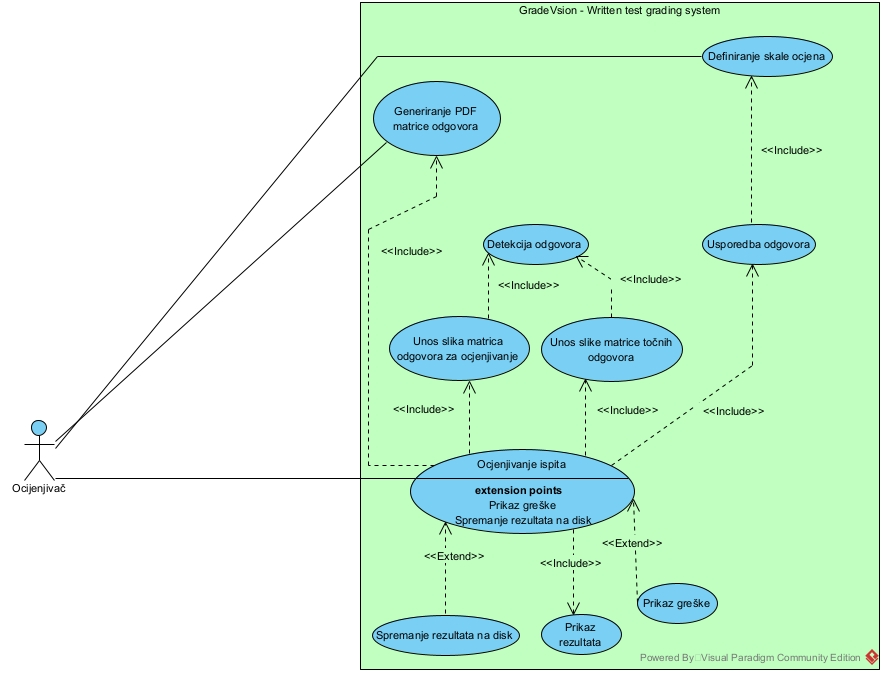
\includegraphics[width=1.0\linewidth]{slike/useCase.jpg}
    \caption{Prikaz Use-case diagrama (Vlastita izrada)}
\end{figure}

\subsection{Slučaj korištenja: Ocjenjivanje ispita}

\subsubsection{Korisnici}
Kao što je već spomenuto, ocjenjivači su jedini korisnici ovog sustava. Oni su u konačnici odgovorni za sam proces ocjenjivanja ispita, a GradeVision softversko rješenje im služi kao alat koji im u tom procesu značajno pomaže. Pomaže im tako što ubrzava sam proces ocjenjivanja, što im omogućuje da više vremena posvete drugim obavezama, poput podizanja kvalitete nastave i sl.

\subsubsection{Glavni scenarij}
Glavni scenarij u ovom sustavu je ocjenjivanje ispita. Ocjenjivač pokreće tu aktivnost, koja zatim uključuje ostale dijelove sustava o kojima ovisi ispravan rad. To su druge aktivnosti poput generiranja PDF matrice odgovora, unosa slika i usporedbe odgovora.

\subsubsection{Uključeni slučaj uporabe: Generiranje PDF matrice odgovora}
Sustav ima mogućnost ocjenjivanja samo onih ispita koji imaju matrice odgovora u određenom formatu, stoga se prije ocjenjivanja ta matrica mora generirati. Taj format je donekle fleksibilan što se tiče broja pitanja i odgovora, ali osnovna struktura mora biti ista. Zbog toga ocjenjivač prije samog ocjenjivanja mora pokrenuti aktivnost "Generiranje PDF matrice odgovora" i definirati broj pitanja i odgovora kako bi kasnije mogao uspješno ocijeniti te matrice. Ako se ovaj korak preskoči i u sustav se učita matrica nekompatibilnog formata, sustav neće raditi.

\subsubsection{Uključeni slučaj uporabe: Unos slike matrice točnih odgovora}
Također, prije ocjenjivanja sustav mora znati koji su točni odgovori kako bi ih kasnije mogao usporediti. Stoga ocjenjivač mora učitati sliku matrice točnih odgovora čime se pokreće aktivnost "Unos slike matrice točnih odgovora".

\subsubsection{Uključeni slučaj uporabe: Unos slika matrica odgovora za ocjenjivanje}
Nakon što sustav ima učitanu sliku matrice točnih odgovora, potrebno je učitati slike matrica odgovora koje treba ocijeniti, jer bez tog koraka sustav ne zna što je potrebno ocijeniti. Učitavanjem tih slika pokreće se aktivnost "Unos slika matrica odgovora za ocjenjivanje".

\subsubsection{Uključeni slučaj uporabe: Detekcija odgovora}
Obje aktivnosti učitavanja matrica odgovora ovise o aktivnosti "Detekcija odgovora", koja je ujedno jedna od najvažnijih aktivnosti koje sustav provodi, budući da se tu nalazi cijela logika za obradu slika i izdvajanje podataka o označenim odgovorima.

\subsubsection{Uključeni slučaj uporabe: Usporedba odgovora}
Nakon što su odgovori s učitanih matrica odgovora detektirani, pokreće se aktivnost "Usporedba odgovora", koja uspoređuje odgovore s matrica za ocjenjivanje s točnim odgovorima iz matrice točnih odgovora. Ta aktivnost također ovisi o aktivnosti "Definiranje skale ocjena", koja definira raspone za postizanje određene ocjene u postocima. U slučaju da skala nije definirana, koristi se unaprijed zadana skala.

\subsubsection{Ostali prošireni i uključeni slučajevi uporabe}
Nakon što je ispit ocijenjen, pokreće se aktivnost "Prikaz rezultata", te po potrebi aktivnosti "Prikaz greške" i "Spremanje rezultata na disk". Zadnje dvije aktivnosti su opcionalne. Spremanje na disk korisnik može uključiti ili isključiti, dok se greške prikazuju samo ako postoje razlike između detektiranih odgovora za ocjenjivanje i točnih odgovora. To mogu biti razlike poput različitog broja pitanja i odgovora i sl.

\subsubsection{Tijek aktivnosti}
\begin{flushleft}
Ovo je pravilan tijek aktivnosti slučaja korištenja "Ocjenjivanje ispita":
\begin{enumerate}
    \item \textbf{Generiranje PDF matrice odgovora} \\
    Ocjenjivač definira broj pitanja i odgovora te generira matricu u propisanom formatu.
    
    \item \textbf{Definiranje skale ocjena} \\
    Ocjenjivač može definirati vlastitu skalu ocjena. Ako se preskoči, koristi se zadana skala.
    
    \item \textbf{Unos slike matrice točnih odgovora} \\
    Učitava se slika ispravno riješenog ispita kako bi sustav prepoznao točne odgovore.
    
    \item \textbf{Unos slika matrica odgovora za ocjenjivanje} \\
    Učitavaju se slike ispita koje je potrebno ocijeniti.
    
    \item \textbf{Detekcija odgovora} \\
    Sustav obrađuje slike i detektira i klasificira odgovore za svako pitanje.
    
    \item \textbf{Usporedba odgovora} \\
    Detektirani odgovori uspoređuju se s točnim odgovorima na temelju zadane skale ocjena.
    
    \item \textbf{Prikaz rezultata} \\
    Korisniku se prikazuju ocjene i vizualna oznaka točnih/netočnih odgovora.
    
    \item \textbf{Spremanje rezultata na disk (ako je uključena opcija)} \\
    Rezultati se mogu trajno pohraniti, ako je uključena ta opcija.
    
    \item \textbf{Prikaz greške (samo ako je potrebno)} \\
    Ako postoji nesukladnost između matrica, poput razlike u broju pitanja ili odgovora, korisnik će biti obavješten o nastanku greške.
\end{enumerate}
\end{flushleft}

\chapter{Dizajn i izrada artefakta}

Kroz ostatak rada fokus će biti na dizajnu i izradi artefakta za opisani problem. Artefakt će biti prikazan kroz različite dijagrame i zanimljive isječke koda.

\section{Odabrane tehnologije}

Prije prikaza samog rješenja, važno je razumjeti koje su tehnologije odabrane i koji su razlozi za njihov odabir. U prijašnjim poglavljima spomenute su relevantne tehnologije, odnosno biblioteke za računalni vid. Analizirane biblioteke mogu se podijeliti na biblioteke za obradu slike i biblioteke za strojno i duboko učenje. Kroz ovaj rad fokus će biti na izradi rješenja isključivo korištenjem obrade slike. Ta odluka donesena je iz osobnih preferencija. Time se izbor automatski sužava na dvije popularne biblioteke: OpenCV i Scikit-Image.

Osim biblioteke, važan je i programski jezik koji je odabran. Budući da je cilj ovog rada izraditi biblioteku otvorenog koda, donesena je odluka koristiti C\# i .NET. Taj programski jezik omogućuje izradu biblioteke u obliku .dll datoteke, kao i jednostavnu izradu demo aplikacije korištenjem WinForms tehnologije, koja je također bazirana na C\#-u i .NET-u.

Odabir programskog jezika ujedno je olakšao i odabir biblioteke za računalni vid. Budući da Scikit-Image ne podržava odabrane tehnologije, odlučeno je koristiti EmguCV. EmguCV je zapravo .NET omotač za OpenCV biblioteku. Odabir EmguCV-a omogućio je korištenje sve postojeće dokumentacije, materijala i više od 2500 metoda vezanih za OpenCV.

Važno je napomenuti da je prije početka dizajna artefakta donesena odluka da sustav mora biti neovisan o konkretnoj biblioteci za računalni vid. To znači da će se korisnicima omogućiti izrada vlastitih implementacija koristeći bilo koju drugu biblioteku za računalni vid.

Kako bi to bilo moguće, odlučeno je koristiti uzorak dizajna injektiranja ovisnosti (eng. dependency injection). Točnije, definirane su apstraktne klase koje korisnici mogu naslijediti i implementirati prema vlastitim potrebama, a zatim ih injektirati u glavnu klasu biblioteke ovog rješenja.
\section{Strukturni model sustava} 


\begin{figure}[H]
    \centering
    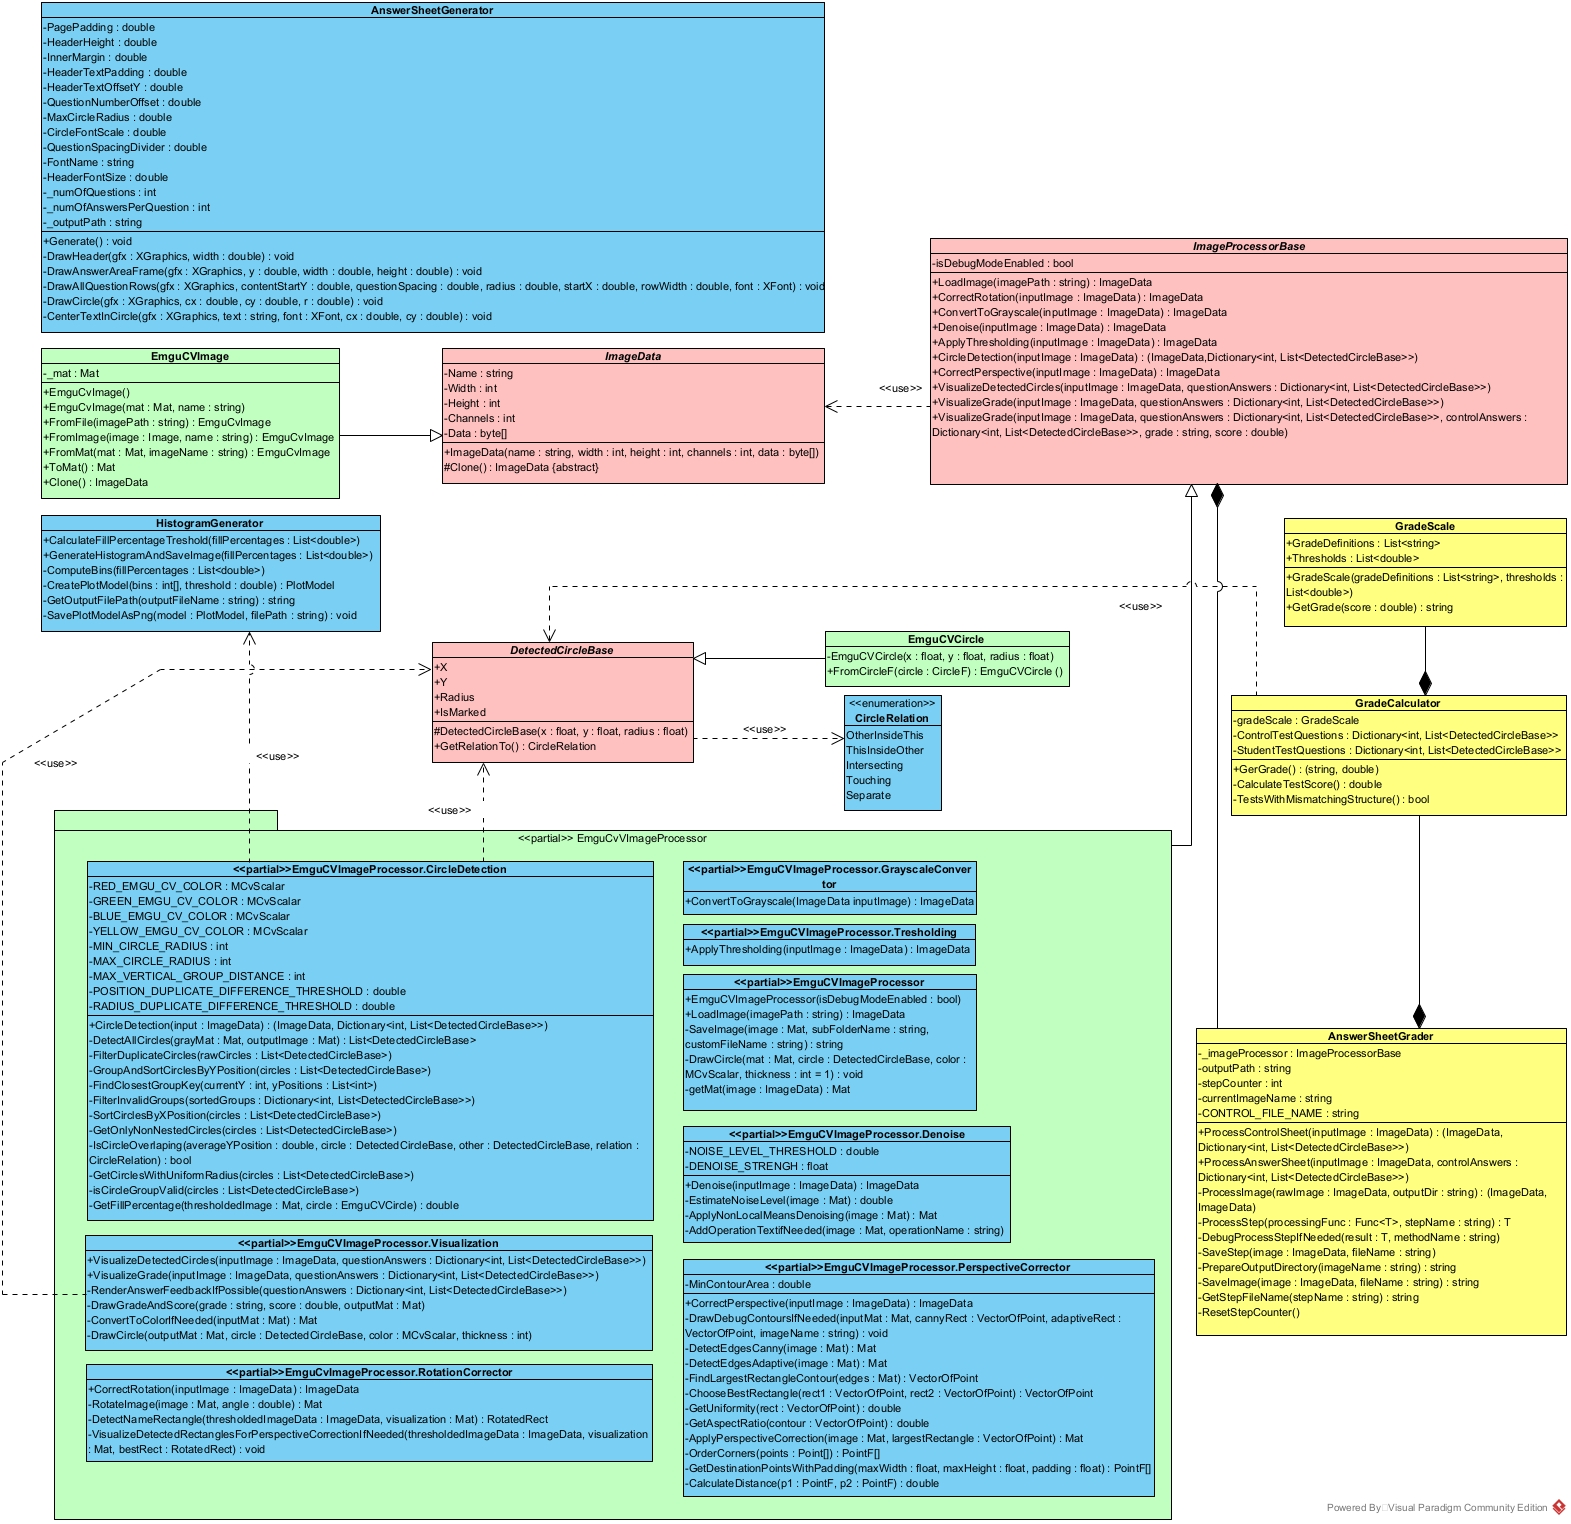
\includegraphics[width=1.0\linewidth]{slike/classDiagram.png}
    \caption{Prikaz dijagrama klasa (Vlastita izrada)}
\end{figure}

Na priloženoj slici prikazana je struktura izrađenog sustava za detekciju odgovora na pismenim ispitima nazvanog GradeVision. Struktura je prikazana korištenjem dijagrama klasa, što omogućuje detaljan uvid u atribute, metode i međuovisnosti svake klase. Klase na ovoj slici možemo podijeliti na klase koje se bave procesiranjem slika i klase temeljne poslovne logike. Nadalje, klase za procesiranje slika mogu se podijeliti na apstraktne i specifične klase.

Apstraktne klase (označene crvenom bojom) su: \texttt{ImageData}, \texttt{DetectedCircleBase} i \texttt{ImageProcessorBase}. U ovom slučaju, te klase postoje kako bi ispunile jedan od nefunkcionalnih zahtjeva (NFZ-02). Taj je zahtjev bio vezan uz jednostavnu zamjenu biblioteka za računalni vid.
Specifične klase (označene zelenom bojom) su: \texttt{EmguCvImage}, \texttt{EmguCvCircle} i \texttt{EmguCvImageProcessor}. One predstavljaju zadanu implementaciju apstraktnih klasa, napisanu korištenjem biblioteke EmguCV za računalni vid.

Važno je napomenuti da klasa \texttt{EmguCvImageProcessor} nasljeđuje apstraktnu klasu \texttt{ImageProcessorBase}, ali ne implementira sve njezine metode u jednoj C\# datoteci. Metode su implementirane u više datoteka koristeći koncept parcijalnih klasa u programskom jeziku C\#. To smanjuje potrebu za implementacijom više sučelja prilikom kreiranja nove implementacije. Klasa \texttt{EmguCvImageProcessor} definirana je kroz sljedeće datoteke, pri čemu svaka datoteka poštuje načelo jedinstvene odgovornosti (\textit{eng. Single Responsibility Principle}):

\begin{itemize}
    \item \textbf{EmguCVImageProcessor.cs}
    \begin{itemize}
        \item Klasa koja sadrži konstruktor te sve zajedničke i pomoćne metode koje nisu specifične samo za jedan korak obrade
    \end{itemize}
    
    \item \textbf{EmguCVImageProcessor.CircleDetection.cs}
    \begin{itemize}
        \item Sadrži logiku za detekciju krugova, njihovo grupiranje, filtriranje i klasificiranje
    \end{itemize}

    \item \textbf{EmguCVImageProcessor.Denoise.cs}
    \begin{itemize}
        \item Sadrži logiku za uklanjanje šuma u slučaju da je razina šuma iznad definiranog praga
    \end{itemize}

    \item \textbf{EmguCVImageProcessor.GrayscaleConvertor.cs}
    \begin{itemize}
        \item Sadrži logiku za pretvorbu slike u boji u sivu sliku
    \end{itemize}

    \item \textbf{EmguCVImageProcessor.PerspectiveCorrector.cs}
    \begin{itemize}
        \item Sadrži logiku za detekciju papira ili unutarnjih okvira ispita te ispravljanje perspektivne deformacije
    \end{itemize}

    \item \textbf{EmguCvImageProcessor.RotationCorrector.cs}
    \begin{itemize}
        \item Sadrži logiku za određivanje orijentacije papira i korekciju pogrešne rotacije
    \end{itemize}

    \item \textbf{EmguCVImageProcessor.Tresholding.cs}
    \begin{itemize}
        \item Sadrži logiku za pretvorbu sive slike u binarnu sliku korištenjem tehnike adaptivnog praga (\textit{engl. Adaptive Thresholding})
    \end{itemize}

    \item \textbf{EmguCVImageProcessor.Visualization.cs}
    \begin{itemize}
        \item Sadrži logiku za vizualizaciju označenih odgovora i ocjena
    \end{itemize}
\end{itemize}


Svi koraci procesiranja slike definirani su unutar klase \texttt{ImageProcessorBase}, a implementirani u klasi \texttt{EmguCvImageProcessor}. Važno je naglasiti da u tim klasama nije definiran ni redoslijed operacija ni logika ocjenjivanja testova. Taj je dio izdvojen u klase (označene žutom bojom): \texttt{AnswerSheetGrader}, \texttt{GradeCalculator} i \texttt{GradeScale}. To su ujedno i klase s kojima bi korisnici biblioteke trebali imati najviše interakcije.

\subsection{Klase ImageData i EmguCvImage}

Kako bi se omogućila zamjena biblioteke za računalni vid, bilo je potrebno koristiti podatkovni model slike koji nije vezan ni uz jednu konkretnu biblioteku. Zbog toga je kreirana apstraktna klasa \texttt{ImageData}, koja sadrži sve potrebne podatke za daljnje procesiranje slike. To uključuje naziv datoteke, širinu, visinu, broj kanala, podatke o slici u obliku niza bajtova te metodu za kloniranje. Na taj način svaka implementacija tog sučelja može biti predstavljena na isti način.

Na primjer, \texttt{EmguCvImage} je implementacija koja predstavlja objekt tipa Mat iz biblioteke EmguCV u obliku \texttt{ImageData}. Također sadrži razne pomoćne metode poput ToMat, FromMat, FromFile i sličnih, što omogućuje još jednostavniji razvoj.

\texttt{ImageData} se koristi u svim dijelovima koda koji moraju biti neovisni o biblioteci za računalni vid, dok se \texttt{EmguCvImage} koristi isključivo u specifičnoj implementaciji koja koristi biblioteku EmguCV.

\subsection{Klase DetectedCircleBase i EmguCvCircle}

\texttt{DetectedCircleBase} je klasa koja je također nastala iz potrebe da sustav bude neovisan o specifičnoj biblioteci za računalni vid. Njezina je svrha pohranjivanje svih podataka o detektiranim krugovima, dok se specifične implementacije poput \texttt{EmguCvCircle} brinu za prikaz specifičnih objekata biblioteke računalnog vida u tom obliku.

\texttt{DetectedCircleBase} sadrži sve važne informacije o detektiranom krugu poput: x koordinate, y koordinate, radijusa i vrijednosti koja označava je li krug ispunjen. Osim toga, sadrži i metodu koja provjerava odnos jednog objekta tipa \texttt{DetectedCircleBase} u odnosu na drugi objekt iste klase. Time se može saznati radi li se o krugu koji se preklapa i slično, što će u daljnjem dijelu rada biti iznimno važno.

\texttt{EmguCvCircle} samo nasljeđuje \texttt{DetectedCircleBase} i omogućuje kreiranje objekta na temelju modela podataka \texttt{CircleF}, koji je prisutan u biblioteci EmguCV.


\subsection{Klasa EmguCvImageProcessor}

Kao što je već spomenuto, \texttt{EmguCvImageProcessor} je konkretna klasa koja implementira metode naslijeđene iz apstraktne klase \texttt{ImageProcessorBase}. Budući da se radi o parcijalnoj klasi, metode su implementirane u različitim datotekama.

Može se reći da je ova klasa zapravo jezgra ovog rješenja. Ona je odgovorna za sve korake koji spadaju pod pretprocesiranje, procesiranje i dio postprocesiranja.

Najvažniji dijelovi logike provode se u fazi pretprocesiranja, budući da se ondje nalazi sva logika koja priprema sliku za daljnju obradu. U toj fazi također su implementirani mehanizmi koji omogućuju da sustav ispravno radi i u uvjetima koji nisu idealni.

Kasnije u radu prikazat će se točan redoslijed tih operacija, koji je definiran klasom \texttt{AnswerSheetGrader}. Također će biti prikazani zanimljivi i nestandardni dijelovi implementacije za svaki od tih koraka.

Sam redoslijed operacija namjerno nije definiran unutar klase \texttt{EmguCvImageProcessor}, budući da je ideja bila izdvojiti što više poslovne logike izvan klasa koje ovise o određenoj biblioteci za računalni vid. Time je omogućeno da se u budućnosti, po potrebi, napiše nova konkretna implementacija klase \texttt{ImageProcessorBase} bez potrebe za ponovnim pisanjem cijele poslovne logike. Može se reći da je u ovom slučaju \texttt{EmguCvImageProcessor} "motor" GradeVision sustava, dok je \texttt{AnswerSheetGrader} "vozač".

\subsection{Klase GradeCalculator i GradeScale}

Klasa \texttt{EmguCvImageProcessor} na kraju obrade slike vraća listu odgovora po pitanjima. Ta lista se zatim predaje klasi \texttt{GradeCalculator}, koja je zadužena za izračun bodova i postotka točnosti ispita, a potom uz pomoć klase \texttt{GradeScale} određuje ocjenu koja će se ispitu dodijeliti.

\texttt{GradeScale} predstavlja unaprijed definiranu skalu ocijena, ali postoji i mogućnost definiranja vlastite skale, što ocjenjivačima pruža dodatnu fleksibilnost.

Unutar ove dvije klase enkapsulirana je sva logika za ocjenjivanje ispita. Trenutna implementacija podržava ocjenjivanje pitanja s jednostrukim i višestrukim odgovorima. Proces bodovanja temelji se na strogoj logici: bod se dodjeljuje samo ako je odgovor u potpunosti točan, to jest nema parcijalnih bodova ni penalizacije za djelomične odgovore.

Važno je napomenuti da ove dvije klase također sudjeluju u fazi postprocesiranja, točnije u konačnom koraku \texttt{Obrada izvučenih podataka}, gdje koriste prethodno definiranu bazu znanja (listu točnih odgovora iz kontrolnog ispita). Nakon toga se ocjene vizualiziraju, a za tu funkcionalnost ponovno je zadužena klasa \texttt{EmguCvImageProcessor}.

\subsection{Ostale klase}

Od ostalih klasa postoje \texttt{HistogramGenerator} i \texttt{AnswerSheetGenerator} klase. Radi se o generatorima sadržaja. Klasa \texttt{AnswerSheetGenerator} odgovorna je za generiranje matrice odgovora prema zadanim parametrima, kao što je definirano u funkcionalnom zahtjevu FZ-02. Za razliku od ostalih klasa, riječ je o potpuno neovisnoj komponenti sustava, čija se metoda \texttt{Generate()} može pozvati u bilo kojem trenutku izvođenja programa, bez utjecaja na njegovo daljnje izvođenje.

S druge strane, klasa \texttt{HistogramGenerator} je pomoćna klasa koja ima ključnu ulogu u procesu detekcije krugova. Implementira algoritam za određivanje praga koji definira je li neki odgovor označen ili nije. Izračunati pragovi se zatim  vizualiziraju i pohranjuju u obliku histograma na disk. Histogrami se spremaju samo kada je program pokrenut u načinu rada za otklanjanje pogrešaka (\textit{engl. debug mode}), koji je definiran u funkcionalnom zahtjevu FZ-06.

Važno je napomenuti da je klasa \texttt{HistogramGenerator} potpuno neovisna o bibliotekama za računalni vid, iako se primarno koristi od strane \texttt{EmguCVImageProcessor} klase. Ona prima listu decimalnih brojeva koji predstavljaju odgovore na ispitnim listovima s određenim postotkom ispunjenosti. Te podatke obrađuje i vraća prag ispunjenosti kruga u obliku postotka. Ako je postotak ispunjenosti viši od izračunatog praga, krug se smatra označenim.

\section{Modeliranje ponašanja sustava}

Kroz sljedeće dijagrame slijeda prikazat će se interakcije između korisnika i različitih dijelova sustava na visokoj razini, dok će se kroz daljnji rad prikazati zanimljivi dijelovi detaljnije. Svaki dijagram slijeda vezan je uz jedan od koraka koje ocjenjivač može napraviti i time pokrenuti neku interakciju sa sustavom.

\subsection{Ponašanje sustava tijekom detekcije odgovora s kontrolnog ispita}

\begin{figure}[H]
\centering
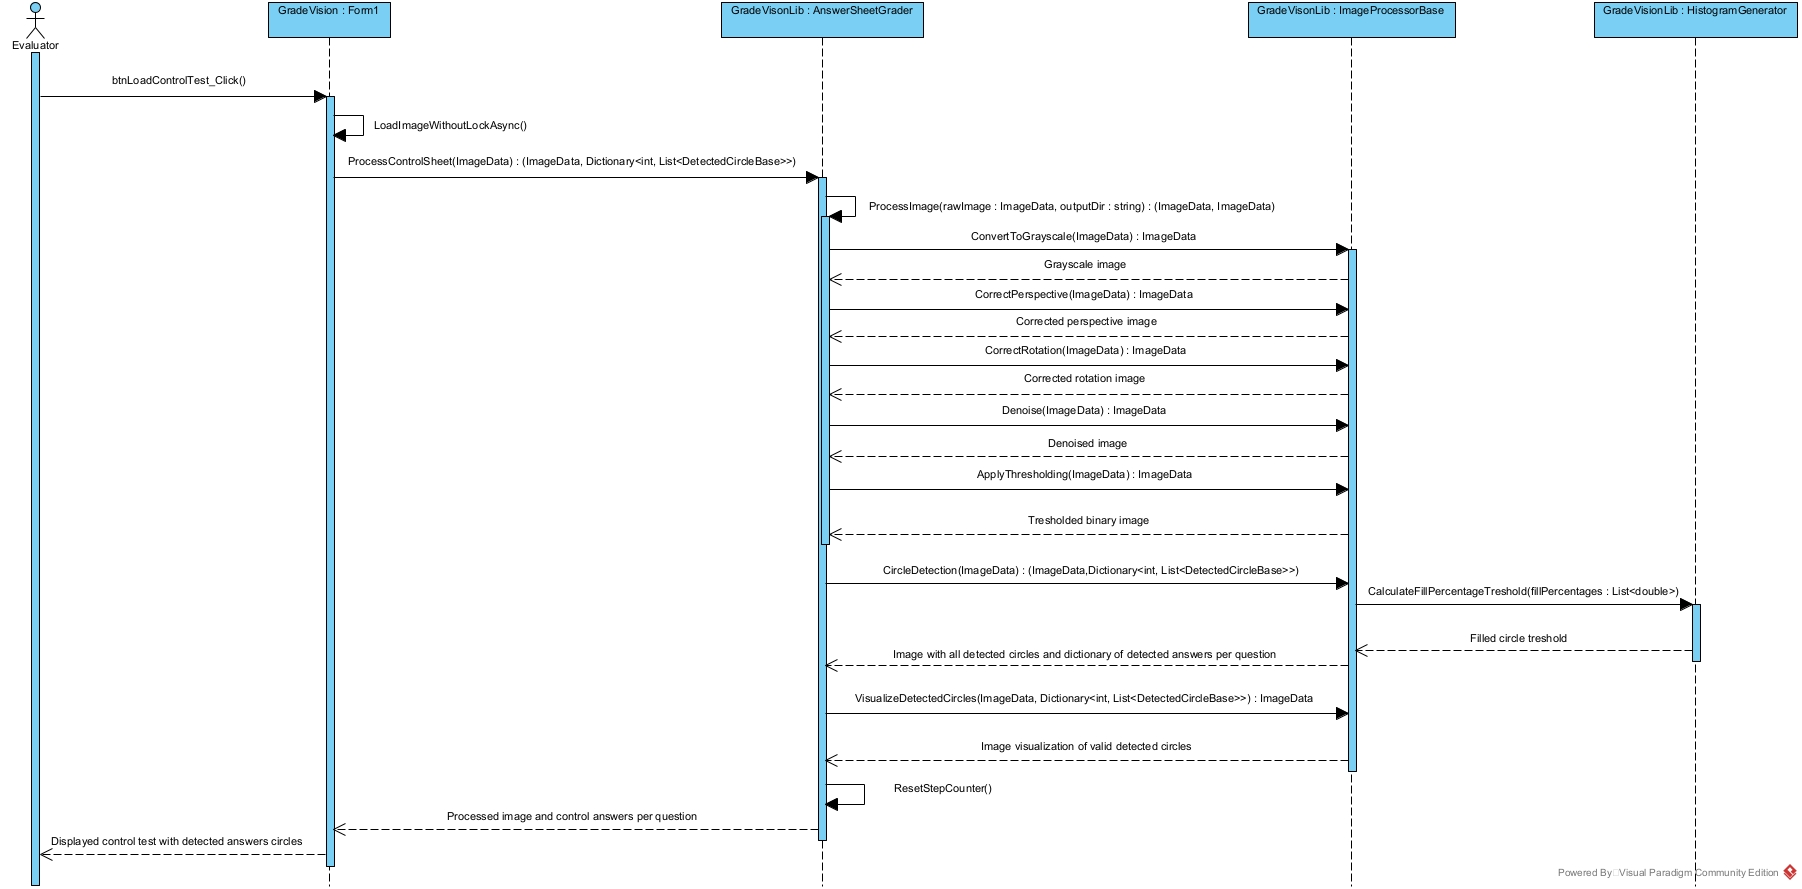
\includegraphics[width=1.0\linewidth]{slike/sequence1.jpg}
\caption{Prikaz dijagrama slijeda za detekciju odgovora s kontrolnog ispita (Vlastita izrada)}
\end{figure}

Dosad se \texttt{GradeVision} spominjao samo kao biblioteka, ali za potrebe testiranja i demonstracije izrađena je jednostavna WinForms aplikacija koja koristi mogućnosti te biblioteke, a koja će se u daljnjem dijelu rada spominjati kao \texttt{GradeVision korisničko sučelje}, dok će se biblioteka spominjati kao \texttt{GradeVisionLib}. Također, u daljnjem dijelu rada spominjat će se pojmovi \texttt{kontrolni ispit} i \texttt{ispit za ocjenjivanje}. Kontrolni ispit označava ispit koji sadrži sve točne odgovore za svako pitanje, dok ispit za ocjenjivanje označava ispit čija je točnost nepoznata te se tek treba utvrditi usporedbom detektiranih odgovora s detektiranim odgovorima kontrolnog ispita (eng. control test).

Priloženi dijagram prikazuje proces detekcije odgovora s kontrolnog ispita. To je vrlo važan proces, budući da je njegov konačni rezultat izrada baze znanja s točnim odgovorima za svako pitanje, koja se kasnije koristi pri ocjenjivanju.

Taj proces pokreće ocjenjivač  tako da učita sliku kontrolnog ispita u \texttt{GradeVision} korisničko sučelje. Zatim aplikacija GradeVision poziva \texttt{AnswerSheetGrader}, koji je dio GradeVisionLib-a. Točnije, poziva se metoda \texttt{ProcessControlSheet(ImageData)}, čime se zapravo pokreće obrada slike. Veći dio obrade slike izvodi se u metodi \texttt{ProcessImage(ImageData rawImage, string outputDir)}, koja orkestrira sve aktivnosti pretprocesiranja pozivanjem metoda konkretne implementacije klase \texttt{ImageProcessorBase} sljedećim redoslijedom:

\begin{itemize}
\item ConvertToGrayscale(image)
\item CorrectPerspective(image)
\item CorrectRotation(image)
\item Denoise(image)
\item ApplyThresholding(image)
\end{itemize}

Naravno ove metode kasnije pozivaju svoje privatne pomoćne metode no to će uvijek ovisiti o biblioteci računalnog vida koja se koristi pa taj dio nije prikazan na dijagramu. Metoda \texttt{ProcessImage(ImageData rawImage, string outputDir)} se također koristi i kod pretprocesiranja ispita za ocijenjivanje što će u nastavku biti prikazano. Važno je napomenuti da je sam  redoslijed aktivnosti pretprocesiranja dobiven kroz opsežno testiranje i iteriranje tijekom razvoja i ova varijanta se pokazala najboljom. Kvaliteta redoslijeda tih aktivnosti bila je mjerena prema preciznosti samog sustava nad skupom podataka vlastite izrade koji će također biti priloženi uz ovaj rad.

Osim toga, metoda \texttt{ProcessImage(ImageData rawImage, string outputDir)}  se također koristi pri pretprocesiranju ispita za ocjenjivanje, što će biti prikazano u nastavku.
Naravno, ove metode kasnije pozivaju svoje privatne pomoćne metode, što će uvijek ovisiti o biblioteci računalnog vida koja se koristi, pa taj dio nije prikazan na dijagramu zbog čitljivosti.

Nakon što je pretprocesiranje završeno, započinje faza procesiranja tako što \texttt{AnswerSheetGrader} poziva metodu \texttt{CircleDetection(ImageData inputImage)}. Metoda \texttt{CircleDetection} jedan je od najvažnijih dijelova ovog rada, budući da se u njoj odvija detekcija odgovora i njihovo klasificiranje u dvije klase: označen i neoznačen odgovor.

Sama logika klasificiranja koristi opisne vrijednosti ispunjenosti objekta, koje izražavaju postotak u kojem je pojedini odgovor ispunjen. Međutim, samo poznavanje postotka ispunjenosti nije dovoljno za ispravnu klasifikaciju odgovora. Potrebno je odrediti prag ispunjenosti koji razdvaja te dvije klase. Taj se prag može postaviti proizvoljno, no takav pristup nije pouzdan jer ne ispunjava svaka osoba krug odgovora na isti način. Osim toga, dodatni čimbenici poput veličine kruga odgovora na papiru također utječu na rezultate.

Zbog toga je bilo potrebno osmisliti preciznije rješenje. Ono je implementirano u klasi \texttt{HistogramGenerator}, unutar metode \texttt{CalculateFillPercentageThreshold(List<double> fillPercentages)}. Upravo se ta metoda poziva unutar \texttt{CircleDetection} metode prije nego što se vrati slika sa svim detektiranim odgovorima i rječnik klasificiranih odgovora grupiranih po pitanjima.

Klasa \texttt{AnswerSheetGrader} zatim poziva metodu \texttt{VisualizeDetectedCircles} iz klase \texttt{ImageProcessorBase} kako bi se klasificirani odgovori vizualizirali. Nakon toga se kreirana slika vraća sve do GradeVision korisničkog sučelja, gdje je prikazana ocjenjivaču. 

\subsection{Ponašanje sustava tijekom ocjenjivanja}

\begin{figure}[H]
\centering
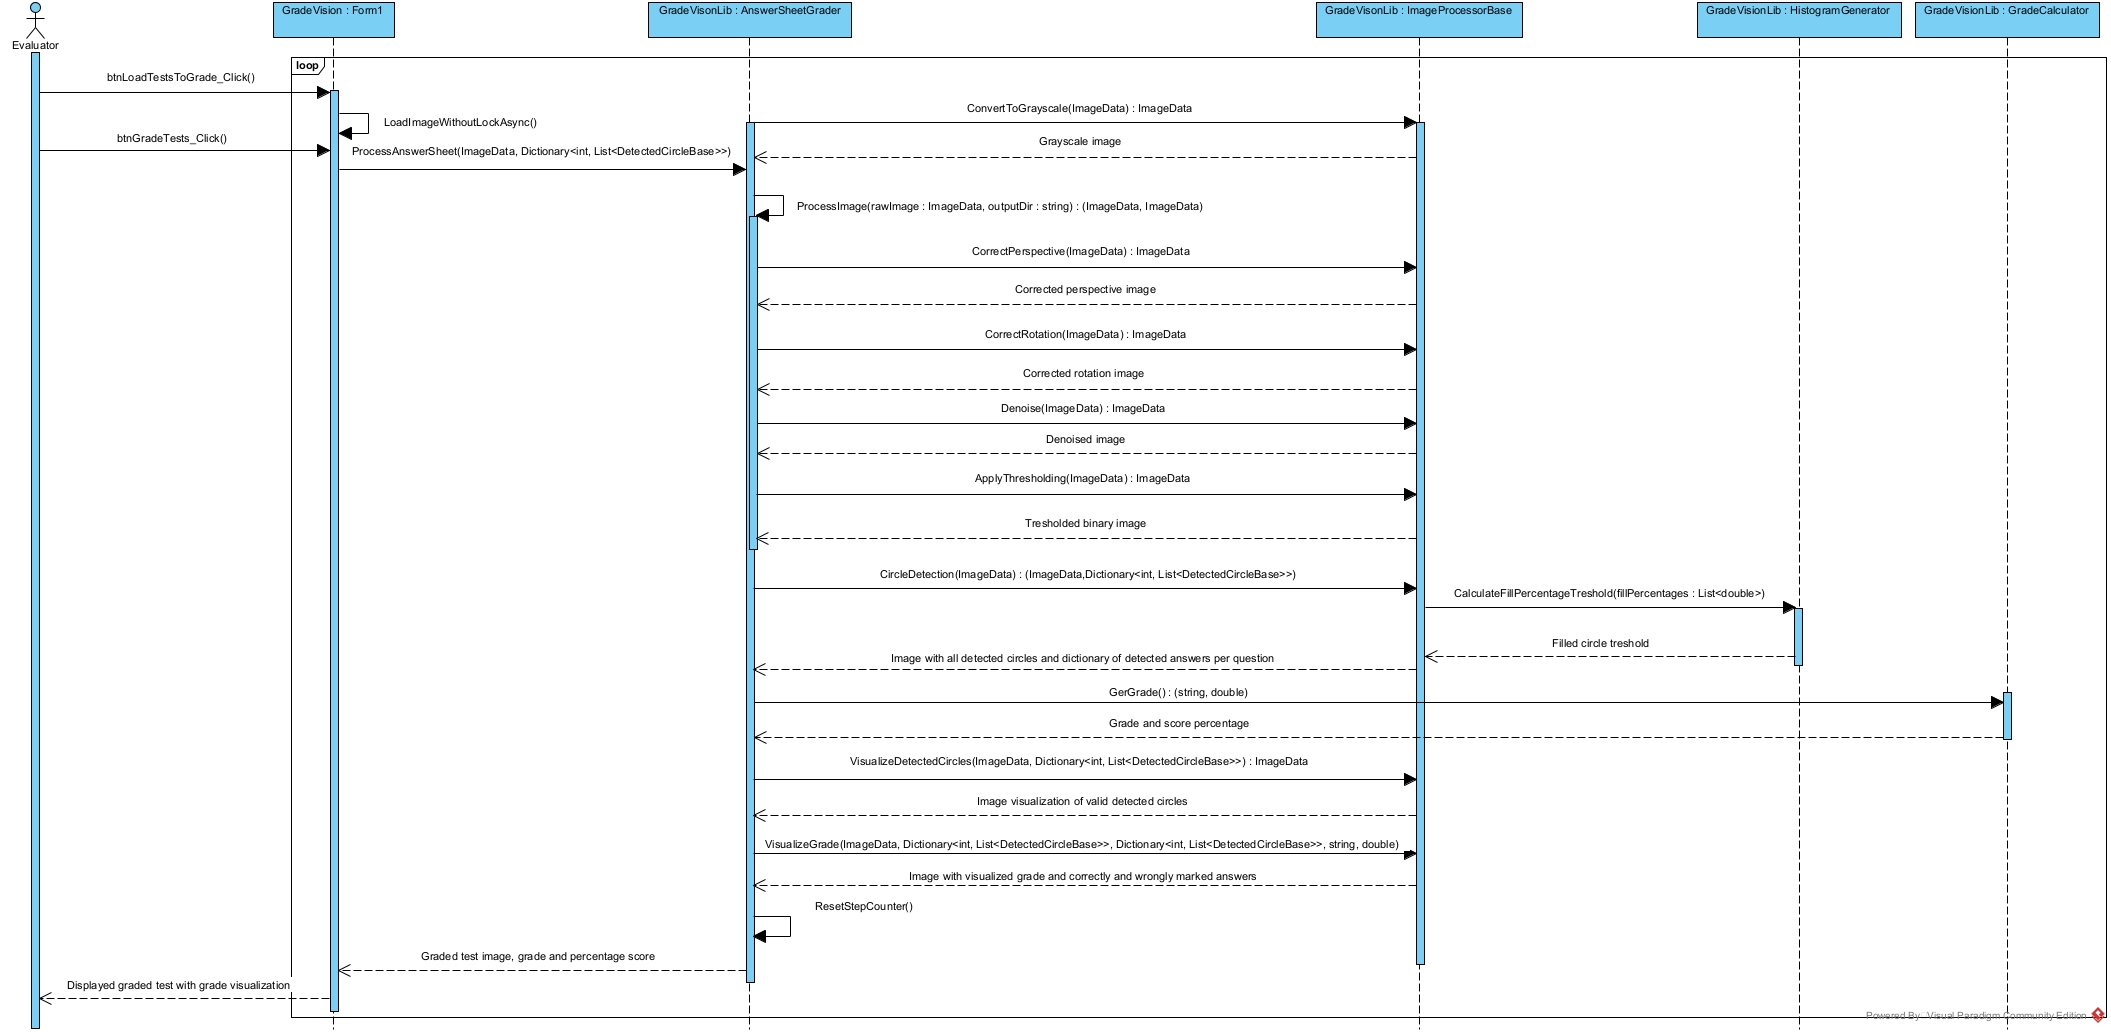
\includegraphics[width=1.0\linewidth]{slike/sequence2.jpg}
\caption{Prikaz dijagrama slijeda ocijenjivanja ispita (Vlastita izrada)}
\end{figure}

Priloženi dijagram ima mnogo sličnosti sa prijašnjim dijagramom slijeda, ali razlikuje se u par ključnih stvari. Prva razlika je da korsnik ne unosi samo jednu sliku u sustav već više njih. Zatim se poziva metoda \texttt{ProcessAnswerSheet(ImageData inputImage, Dictionary<int, List<DetectedCircleBase>> controlAnswers, GradeScale gradeScale)} koja procesira ispite za ocijenjivanje. Pretprocesiranje ponovno provodi \texttt{ProcessImage(ImageData rawImage, string outputDir)} metoda već spomenutim koracima i redoslijedom. Zatim se provodi detektiranje krugova koje je također već spomenuto, no tu sve sličnosti sa prijašnjim dijagramom završavaju. Nakon detektiranja krugova poziva se \texttt{GradeCalculator} klasa, točnije njezina metoda \texttt{GetGrade()}.

Nakon što metoda vrati ocjenu i postotak riješenosti, poziva se sljedeći korak. Taj korak uključuje vizualizaciju ocjene na način da se na ispitu označe točno i krivo označeni odgovori te da se u gornjem desnom kutu slike napiše postotak i ocjena. Zatim se slika sa vizualizacijom ocjene vraća na ekran ocjenjivača i ponavlja se isti proces za ostale ispite koji još nisu ocijenjeni.

Važno je napomenuti da se ovaj slijed ne može pokrenuti dok god se ne izvrše svi koraci iz prvog dijagrama slijeda za kontrolni ispit. Također, generalna struktura ispita za ocijenjivanje se mora poklapati sa kontrolnim ispitom, pod to spada isti broj pitanja i odgovora.

\subsection{Dijagram slijeda – Generiranje matrice odgovora}

\begin{figure}[H]
\centering
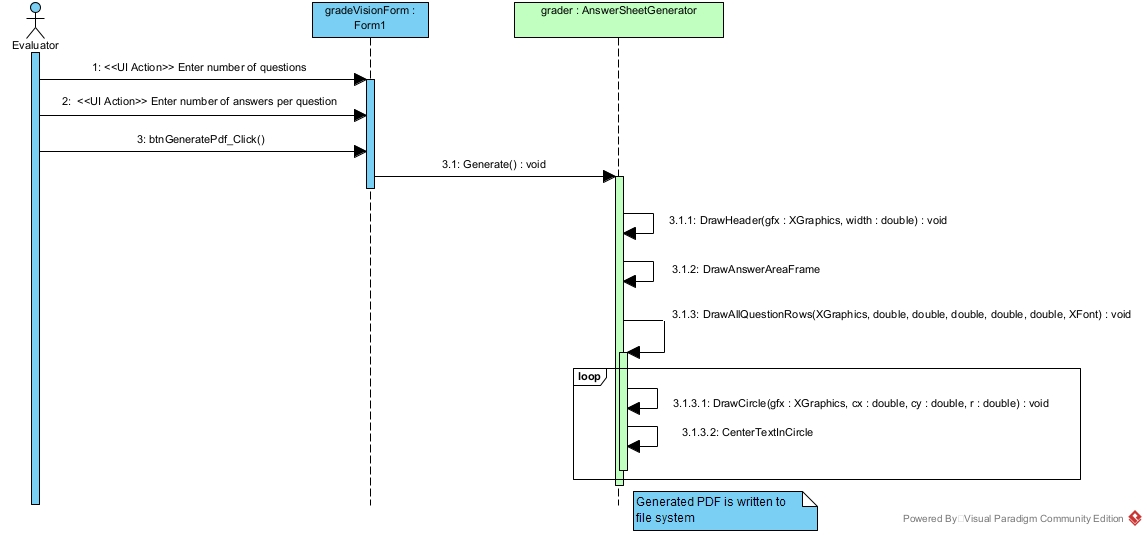
\includegraphics[width=1.0\linewidth]{slike/sequence3.jpg}
\caption{Prikaz dijagrama slijeda za generiranje PDF matrice odgovora (vlastita izrada)}
\end{figure}

Kroz priloženi dijagram slijeda može se vidjeti da je samo generiranje matrice odgovora u obliku PDF-a prilično jednostavno. Kako bi se PDF generirao, korisnik najprije mora definirati ukupan broj pitanja i broj ponuđenih odgovora po pitanju. Nakon što su ti parametri definirani, pritišće se gumb za generiranje PDF-a, čime se daljnja kontrola nad izvođenjem predaje klasi forme u WinForm aplikaciji. Ta klasa zatim poziva metodu \texttt{Generate()} klase \texttt{AnswerSheetGenerator}. 

Metoda \texttt{Generate} je metoda bez povratnog tipa podataka, što nije problem jer ona izravno generirani PDF sprema na disk. Metoda \texttt{Generate} poziva svoje privatne metode sljedećim redoslijedom:

\begin{itemize}
\item \texttt{DrawHeader} - Crta pravokutni okvir na vrhu stranice i ispisuje tekst s poljima za ime i ocjenu osobe koja piše ispit.
\item \texttt{DrawAnswerAreaFrame} - Crta pravokutni okvir koji označava područje u kojem se nalaze pitanja i odgovori.
\item \texttt{DrawAllQuestionRows} - Ispisuje redove s brojevima pitanja i pripadajućim krugovima za svaki ponuđeni odgovor.
    \begin{itemize}
    \item \texttt{DrawCircle} - Crta jedan krug koji predstavlja ponuđeni odgovor.
    \item \texttt{CenterTextIntoCircle} - Centrira i ispisuje pripadajuće slovo unutar prethodno nacrtanog kruga.
    \end{itemize}
\end{itemize}


\section{GradeVision aplikacija}

Cilj ovog rada je izrada biblioteke za detekciju odgovora, no kako bi se ista mogla testirati i demonstrirati, izrađena je GradeVision stolna aplikacija. Aplikacija je izrađena korištenjem .NET Core, C\# i WinForms tehnologija. Te su tehnologije odabrane zbog jednostavnosti i brzine izrade demo aplikacije, ali i zato što je i GradeVision biblioteka napisana korištenjem .NET Core i C\#.

\begin{figure}[H]
\centering
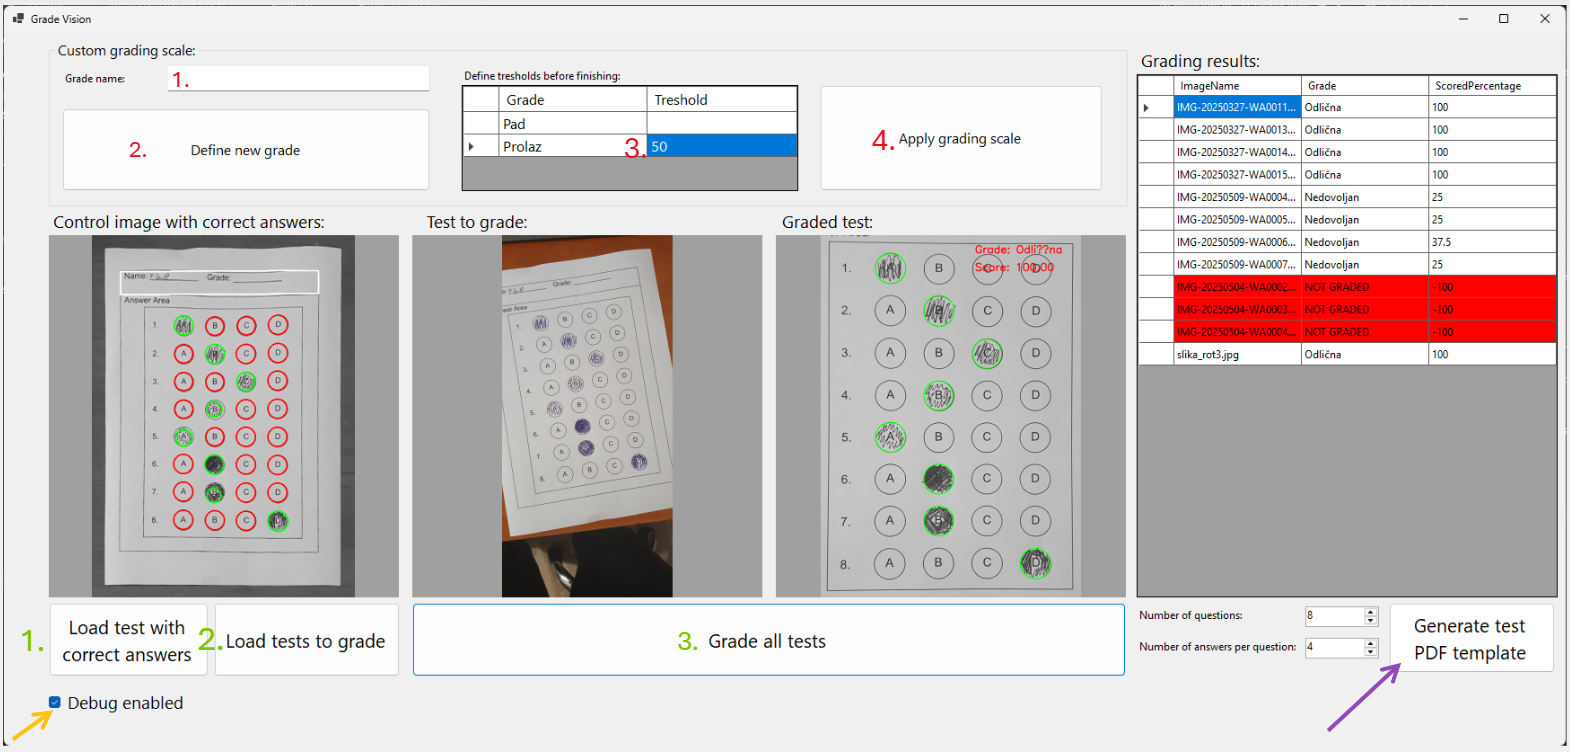
\includegraphics[width=1.0\linewidth]{slike/GradeVision ui.png}
\caption{Prikaz korisničkog sučelja GradeVision stolne demo aplikacije (vlastita izrada)}
\end{figure}

Korisničko sučelje s priložene slike možda na prvi pogled djeluje komplicirano, no zapravo je poprilično jednostavno i sadrži sve potrebne elemente za testiranje i demonstraciju rada biblioteke. Glavni elementi korisničkog sučelja su tri okvira za prikaz slika. Prvi okvir prikazuje kontrolni ispit koji se, nakon učitavanja i ocjenjivanja, prikazuje na tom mjestu. U drugom okviru nalazi se izvorna slika koja se ocjenjuje, dok se desno od nje prikazuje ocijenjena verzija te slike. Također, s desne strane nalazi se i tablica koja prikazuje povijest ocjenjivanja.

Osim tih elemenata, u gornjem lijevom kutu nalaze se kontrole za definiranje nove skale ocjenjivanja, ako je to potrebno. U donjem desnom kutu nalaze se parametri matrice odgovora i gumb za njezino generiranje. Također u doljnjem lijevom kutu postoji gumb za uključivanje i isklučivanje načina rada za otklanjanje grešaka.

\subsection{Način rada}

GradeVison demo aplikacija vrlo je jednostavna za korištenje. Na slici 22 označeni su koraci za korištenje raznih funkcionalnosti aplikacije.

Kako bi se prikazala cjelokupna funkcionalnost aplikacije, najbolje je za početak generirati PDF predložak matrice odgovora. Za generiranje predloška potrebno je u donjem desnom kutu aplikacije odabrati broj pitanja i broj odgovora po pitanju. Zatim je potrebno pritisnuti gumb Generate, koji će generirati PDF matricu odgovora i spremiti je na radnu površinu računala u mapu \texttt{ProcessedImages}. Važno je napomenuti da PDF matrica ima određenu razinu fleksibilnosti što se tiče broja pitanja i odgovora, no broj pitanja je ograničen na minimalno 8, a maksimalno 20, dok je minimalan broj odgovora 4, a maksimalan 8.

Nakon što je matrica odgovora generirana, potrebno ju je isprintati i podijeliti pristupnicima ispita na rješavanje. Osim toga, ocjenjivač treba jednu matricu odgovora riješiti potpuno točno. Slijedi fotografiranje matrica odgovora i unos slika matrica u sustav.

Za unos kontrolne matrice u sustav potrebno je u donjem lijevom kutu aplikacije pritisnuti gumb \texttt{Load test with correct answers} i zatim u datotečnom sustavu odabrati fotografiju kontrolne matrice. Čim se slika učita, automatski se pokreće proces detekcije označenih odgovora na matrici. Kada taj proces završi, izvorna slika u prvom okviru zamjenjuje se slikom s detektiranim odgovorima. Time se omogućuje ocjenjivaču uvid u rad sustava i provjera njegove ispravnosti.

Nakon unosa kontrolne matrice potrebno je unijeti slike matrica odgovora polaznika. Za to je potrebno pritisnuti gumb \texttt{Load tests to grade} i zatim u datotečnom sustavu odabrati slike matrica koje je potrebno ocijeniti. Nakon što su matrice učitane, potrebno je pritisnuti gumb \texttt{Grade all tests}, koji pokreće detekciju odgovora i ocjenjivanje matrica polaznika. Ocijenjeni ispiti vizualiziraju se tijekom ocjenjivanja, a rezultati se upisuju u tablicu na desnoj strani aplikacije. U slučaju da je potrebna dodatna vizualizacija cijelog procesa, moguće je uključiti \texttt{debug mode} klikom na potvrdni okvir u donjem lijevom kutu.

U slučaju da korisnik nije definirao vlastitu skalu ocjenjivanja, sustav koristi unaprijed definiranu skalu:

\begin{table}[h!]
\centering
\begin{tabular}{|c|r|}
\hline
\textbf{Ocjena} & \textbf{Prag (\%)} \\
\hline
1 & < 50 \\
2 & 50 \\
3 & 63 \\
4 & 75 \\
5 & 85 \\
\hline
\end{tabular}
\caption{Unaprijed definirane ocjene i odgovarajući pragovi u obliku postotka}
\end{table}

Osim prikazanih ocjena u tablici, postoji i posebna ocjena \texttt{NOT GRADED}, koja se dodjeljuje u slučaju kada sustav zaključi da nije moguće usporediti matricu polaznika s kontrolnom matricom, iz nekog razloga.

Ako ocjenjivač želi koristiti vlastitu skalu ocjenjivanja, i to je moguće. Potrebno je u gornjem lijevom kutu aplikacije upisati ime ocjene i zatim pritisnuti gumb \texttt{Define new grade}. Taj je postupak potrebno ponoviti više puta, ovisno o broju ocjena koje je potrebno definirati. Nakon što su ocjene definirane, pragovi se dodjeljuju u tablici ocjena i pragova. Prag se dodaje tako da se upiše u tablicu pod stupac \texttt{Threshold}. Važno je napomenuti da se za prvu, tj. negativnu ocjenu, ne može definirati prag — njezin prag je automatski manji od druge definirane ocjene.

Kada je skala definirana u tablici, potrebno je pritisnuti gumb \texttt{Apply grading scale} i ponovno pokrenuti proces ocjenjivanja, koji će se zatim odvijati prema novoj skali.

\section{Značajni dijelovi koda GradeVison biblioteke}

Kroz ovo poglavlje fokus je na prikazu interesantnih dijelova koda GradeVision biblioteke. Sama analiza prolazit će kroz redoslijed operacija prikazan na dijagramu slijeda na slici 20, a fokus će većinski biti na analizi implementacije metoda \texttt{ImageProcessorBase} koristeći EmguCV biblioteku.

Prvi korak procesiranja slike je pretvorba slike u boji u sivu sliku. Za to je odgovorna metoda \texttt{ConvertToGrayscale}:

\begin{lstlisting}[caption={Metoda za konverziju slike u boji u sivu sliku}]
override public ImageData ConvertToGrayscale(ImageData inputImage){
    var inputMat = getMat(inputImage);
    Mat grayMat = new Mat();
    CvInvoke.CvtColor(inputMat, grayMat, ColorConversion.Bgr2Gray);
    return EmguCvImage.FromMat(grayMat, inputImage.Name);
}
\end{lstlisting} 

Priložena metoda zapravo je prvi korak pretprocesiranja slike. Metoda prvo iz apstraktne klase \texttt{InputImage} izvlači \texttt{Mat} objekt, koji je zapravo reprezentacija slike u EmguCV biblioteci. Zatim se pomoću operacije \texttt{CvInvoke.CvtColor} početna matrica pretvara u matricu sive slike koristeći mod konverzije \texttt{ColorConversion.Bgr2Gray}. Na priloženoj slici moguće je vidjeti ulaz i izlaz \texttt{ConvertToGrayscale} metode.

\begin{figure}[H]
\centering
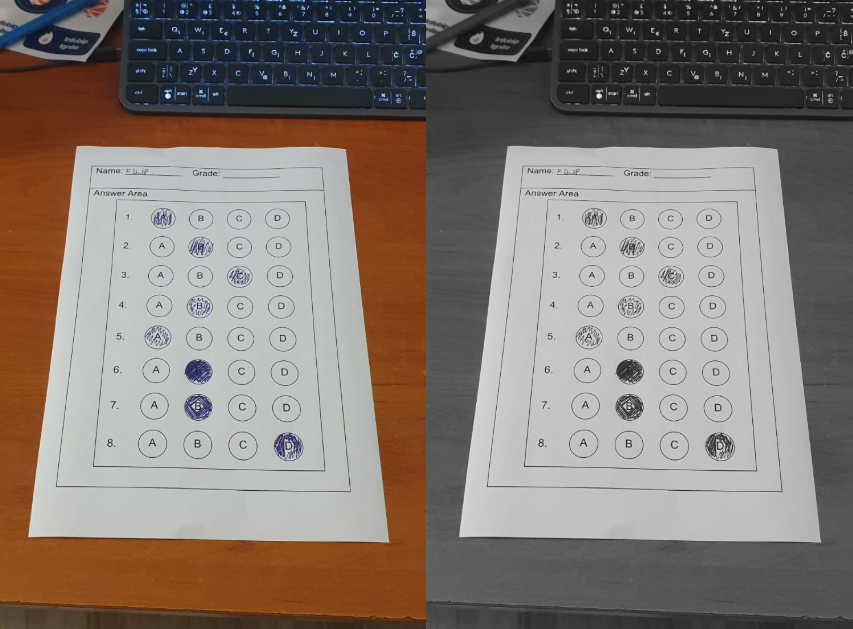
\includegraphics[width=0.8\linewidth]{slike/ToGrayscale.png}
\caption{Prikaz ulazne i izlazne slike ConvertToGrayscale metode (vlastita izrada)}
\end{figure}

Pretvorba u sivu sliku bila je logični prvi korak obrade slike, pošto su za detekciju odgovora boje nebitna komponenta, tako da su odmah na početku uklonjene kako bi se smanjila količina informacija za obradu. Zatim je bilo potrebno odrediti sljedeće korake. Očito je bilo da će biti potrebno smanjiti šum na slici te ispraviti perspektivu i orijentaciju papira nastalu tijekom pribavljanja fotografije, no nije bilo jasno koji je najefikasniji redoslijed tih operacija. Za početak je odabrano smanjenje buke kao sljedeća operacija, ta odluka se evaluirala i mijenjala kroz razvoj artefakta.

\begin{lstlisting}[caption={Metoda za smanjenje buke na slici}]
override public ImageData Denoise(ImageData inputImage){
    var inputMat = getMat(inputImage);
    var noiseLevel = EstimateNoiseLevel(inputMat);

    if (noiseLevel >= NOISE_LEVEL_THRESHOLD){
        inputMat = ApplyNonLocalMeansDenoising(inputMat);
        AddOperationTextifNeeded(inputMat, $"{noiseLevel:F2} NL-Means");
    }
    else{
        AddOperationTextifNeeded(inputMat, $"{noiseLevel:F2} No Denoise");
    }

    return EmguCvImage.FromMat(inputMat, inputImage.Name);
}
\end{lstlisting}

Metoda \texttt{Denoise} odgovorna je za analizu buke na slici pomoću metode \texttt{EstimateNoiseLevel} i uklanjanje buke pomoću metode \texttt{ApplyNonLocalMeansDenoising}. Buka se smanjuje samo u slučaju da je vrijednost veća od definiranog praga \texttt{NOISE\_LEVEL\_THRESHOLD}. U slučaju da je buka ispod tog praga, smatra se da se radi o dozvoljenoj razini buke, to jest razini koja ne bi trebala imati utjecaja na daljnju obradu slike. Taj prag pažljivo je kalibriran tijekom razvoja. Također, ova metoda odgovorna je za prikaz teksta o razini buke i provedenoj operaciji uklanjanja buke. Taj se tekst prikazuje na slici samo ako je sustav u načinu rada za otkrivanje grešaka.

\begin{lstlisting}[caption={Procjena razine buke na slici}]
private double EstimateNoiseLevel(Mat image){
    using (Mat temp = new Mat()){
        CvInvoke.MedianBlur(image, temp, 3);
        CvInvoke.Subtract(image, temp, temp);
        temp.ConvertTo(temp, DepthType.Cv32F);

        var mean = new MCvScalar();
        var stddev = new MCvScalar();
        CvInvoke.MeanStdDev(temp, ref mean, ref stddev);
        return stddev.V0;
    }
}
\end{lstlisting}

Priloženi isječak koda odgovoran je za procjenu buke spomenutu u prijašnjem isječku. Procjena buke izvodi se tako da se na pomoćnom \texttt{Mat} objektu smanji buka pomoću metode \texttt{CvInvoke.MedianBlur}, a zatim se metodom \texttt{CvInvoke.Subtract} oduzmu \texttt{Mat} objekti te se nad rezultatom pronađe standardna devijacija. Važno je napomenuti da ova metoda daje dobre rezultate za sitnu buku visoke frekvencije, što je u ovom slučaju i potrebno. Rezultat ove metode naknadno se uspoređuje s definiranim pragom i utvrđuje se je li potrebno provesti operaciju uklanjanja buke. Ako je potrebno, tada se izvršava metoda iz sljedećeg isječka.

\begin{lstlisting}[caption={Metoda za smanjenje buke}]
private Mat ApplyNonLocalMeansDenoising(Mat image){
    var result = new Mat();
    CvInvoke.FastNlMeansDenoising(image, result,
        h: DENOISE_STRENGH,
        templateWindowSize: 5,
        searchWindowSize: 15);
    return result;
}
\end{lstlisting}

Priložena metoda smanjuje buku koristeći metodu \texttt{CvInvoke.FastNlMeansDenoising}. Radi se o algoritmu poznatom po očuvanju detalja i smanjenju buke, posebno na fotografijama sa sitnim detaljima. Odluka za korištenje ovog algoritma donesena je kroz testiranje raznih algoritama i usporedbu preciznosti cijelog sustava. Na kraju je odlučeno da je ovo najkonzistentnija opcija. Metoda \texttt{CvInvoke.FastNlMeansDenoising} prima tri argumenta koja opisuju jačinu uklanjanja buke i veličinu matrice za pretraživanje i usporedbu blokova piksela.


\begin{figure}[H]
\centering
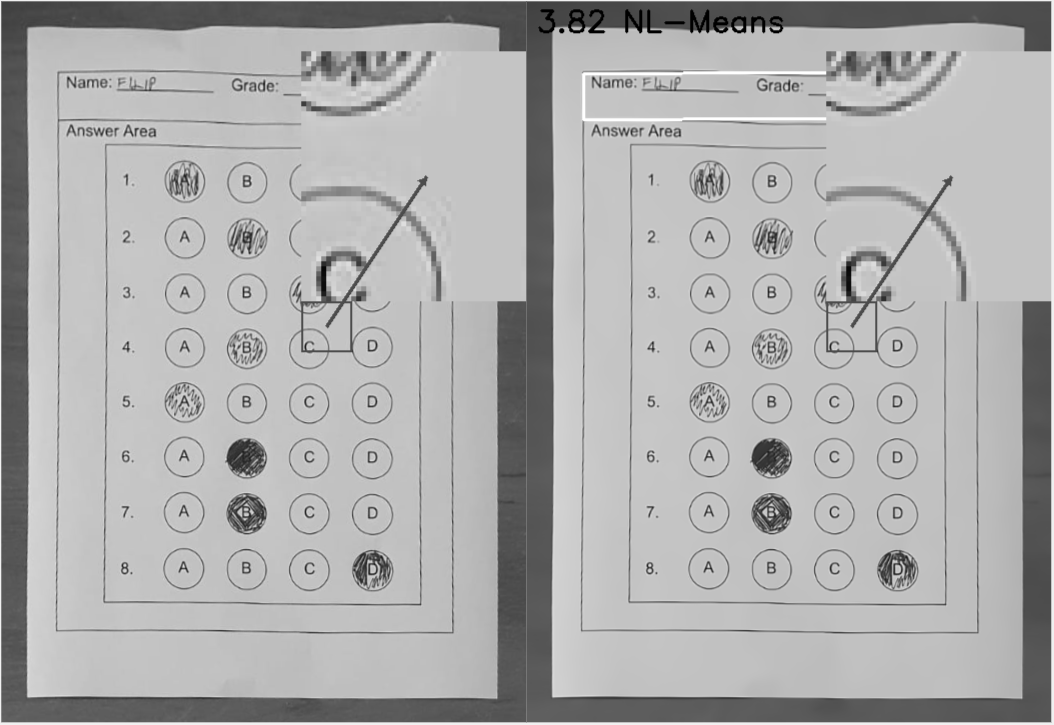
\includegraphics[width=0.8\linewidth]{slike/DenoiseComparison.png}
\caption{Prikaz ulazne i izlazne slike Denoise metode (vlastita izrada)}
\end{figure}

Sa prikazane slike vidljivo je da je buka analizirana i procijenjena kao 3.82, što je iznad definiranog praga, te se primijenila metoda za uklanjanje buke. Razlika u razini buke najbolje je vidljiva na području oko papira i na povećanim sekcijama. Nepotrebna sitna buka na pozadini papira uklonjena je, dok su strukturni elementi ostali većinski očuvani. Smanjenje buke je izrazito važno jer olakšava daljnju obradu slike.

Nakon smanjenja buke, sljedeća faza bila je ispravak perspektive, a zatim ispravak rotacije, to jest orijentacije. Ispravak perspektive bio je jedan od najizazovnijih dijelova ovog rada. Izazov je predstavljala odluka da matrica odgovora neće sadržavati nikakve posebne oznake, poput oznaka za kutove i orijentaciju papira. Zbog toga je bilo potrebno detektirati obrub papira i prema tome ispraviti perspektivu. Kroz priložene isječke prikazani su samo najvažniji i zanimljiviji isječci koda za ispravak perspektive.  

\begin{lstlisting}[caption={Metoda za ispravak perspektive slike}]
override public ImageData CorrectPerspective(ImageData inputImage){
    var inputMat = getMat(inputImage);
    Mat cannyEdges = DetectEdgesCanny(inputMat);
    Mat adaptiveEdges = DetectEdgesAdaptive(inputMat);

    VectorOfPoint cannyRect = FindLargestRectangleContour(cannyEdges);
    VectorOfPoint adaptiveRect = FindLargestRectangleContour(adaptiveEdges);

    DrawDebugContoursIfNeeded(inputMat, cannyRect, adaptiveRect, inputImage.Name);
    VectorOfPoint bestRect = ChooseBestRectangle(cannyRect, adaptiveRect);

    if (bestRect == null)
        return EmguCvImage.FromMat(inputMat, inputImage.Name);

    return EmguCvImage.FromMat(ApplyPerspectiveCorrection(inputMat, bestRect), inputImage.Name);
}
\end{lstlisting}

Iz priloženog koda vidljivo je da se pokušavaju detektirati rubovi svih struktura na slici koristeći dvije različite metode: \texttt{DetectEdgesCanny} i \texttt{DetectEdgesAdaptive}. Zatim se pokušavaju pronaći dvije najveće pravokutne konture koje odgovaraju veličini papira. Zatim se pomoću metode \texttt{ChooseBestRectangle} zaključuje koji je pravokutnik bolji odabir za ispravak perspektive, te se perspektiva ispravlja pomoću metode \texttt{ApplyPerspectiveCorrection}.

Zanimljivost ove metode je u tome što zapravo koristi dva različita pristupa za detekciju rubova. Analiza sljedećih isječaka prikazuje primijenjene metode i objašnjava prednosti i mane oba pristupa.

\pagebreak
\begin{lstlisting}[caption={Metoda za detekciju rubova tijekom ispravka perspektive}]
private Mat DetectEdgesCanny(Mat image){
    Mat edges = new Mat();
    CvInvoke.Canny(image, edges, 50, 150);

    Mat dilatedEdges = new Mat();
    Mat structuringElement = CvInvoke.GetStructuringElement(ElementShape.Rectangle, new Size(3, 3), new Point(1, 1));
    CvInvoke.Dilate(edges, dilatedEdges, structuringElement, new Point(-1, -1), 1, BorderType.Reflect, new MCvScalar(1));

    return dilatedEdges;
}

private Mat DetectEdgesAdaptive(Mat image){
    Mat thresh = new Mat();
    CvInvoke.AdaptiveThreshold(image, thresh, 255, AdaptiveThresholdType.GaussianC, ThresholdType.BinaryInv, 11, 2);

    Mat morph = new Mat();
    Mat kernel = CvInvoke.GetStructuringElement(ElementShape.Rectangle, new Size(3, 3), new Point(-1, -1));
    CvInvoke.MorphologyEx(thresh, morph, MorphOp.Close, kernel, new Point(-1, -1), 2, BorderType.Default, new MCvScalar());

    return morph;
}
\end{lstlisting}

Glavna razlika između priloženih metoda je odabrani pristup za detektiranje rubova.

Metoda \texttt{DetectEdgesCanny} naglašava sve rubove na slici koristeći \texttt{CvInvoke.Canny} algoritam uz pomoć morfološke operacije dilatacije, koja omogućuje spajanje prekinutih rubova, što povećava preciznost sustava u ekstremnim uvjetima.

Metoda \texttt{DetectEdgesAdaptive} ne koristi standardni pristup detektiranju rubova, već koristi \texttt{CvInvoke.AdaptiveThreshold} algoritam koji pretvara ulaznu sivu sliku u binarnu sliku. Ova implementacija namijenjena je specifično kreiranju binarne slike u varijabilnim uvjetima osvjetljenja. Nakon binarizacije, detektiraju se strukturni elementi te se nad njima izvršava morfološka operacija zatvaranja kako bi se povezale i očistile strukturne komponente slike.


Nakon što su rubovi detektirani, započinje proces analize rubova i pronalaska pravokutnika koji najbolje opisuje rub papira na slici. Za to služi metoda \texttt{FindLargestRectangleContour}:

\pagebreak
\begin{lstlisting}[caption={Metoda za pronalazak najvećeg pravokutnika koji predstavlja papir}]
private VectorOfPoint FindLargestRectangleContour(Mat edges){
    using (VectorOfVectorOfPoint contours = new VectorOfVectorOfPoint()){
        CvInvoke.FindContours(edges, contours, null, RetrType.List, ChainApproxMethod.ChainApproxSimple);
        double maxArea = 0;
        VectorOfPoint largestRectangle = null;
        for (int i = 0; i < contours.Size; i++){
            using (VectorOfPoint contour = contours[i])
            {
                double area = CvInvoke.ContourArea(contour);
                if (area < MinContourArea) continue;
                using (VectorOfPoint approx = new VectorOfPoint()){
                    CvInvoke.ApproxPolyDP(contour, approx, 0.02 * CvInvoke.ArcLength(contour, true), true);
                    if (approx.Size == 4 && area > maxArea){
                        maxArea = area;
                        largestRectangle = new VectorOfPoint(approx.ToArray());
                    }
                }
            }
        }
        return largestRectangle;
    }
}
\end{lstlisting}

Ova metoda funkcionira tako da pomoću metode \texttt{CvInvoke.FindContours} pronalazi sve konture na slici. Zatim se izračunava površina konture pomoću \texttt{CvInvoke.ContourArea}. Ako je površina manja od unaprijed definirane minimalne vrijednosti \texttt{MinContourArea}, kontura se preskače. U slučaju da je površina dovoljno velika, kontura se aproksimira u poligon pomoću metode \texttt{CvInvoke.ApproxPolyDP}. Taj aproksimirani poligon mora imati točno četiri vrha, tj. mora biti pravokutnik. Ako je takav pravokutnik veći od prethodno pronađenog najvećeg, tada se postavlja kao novi najveći pravokutnik.


Nakon što su izračunata dva najveća pravokutnika prema podacima iz metoda \texttt{DetectEdgesCanny} i \texttt{DetectEdgesAdaptive}, potrebno je odlučiti koji je pravokutnik zapravo najviše sličan obrisu papira. Za to se koristi metoda \texttt{ChooseBestRectangle}:
\pagebreak
\begin{lstlisting}[caption={Metoda za odabir najboljeg pravokutnika}]
private VectorOfPoint ChooseBestRectangle(VectorOfPoint rect1, VectorOfPoint rect2){
    if (rect1 == null) return rect2;
    if (rect2 == null) return rect1;
    var area1 = CvInvoke.ContourArea(rect1);
    var area2 = CvInvoke.ContourArea(rect2);
    var aspect1 = GetAspectRatio(rect1);
    var aspect2 = GetAspectRatio(rect2);
    var isValid1 = aspect1 is > 0.5 and < 2.0;
    var isValid2 = aspect2 is > 0.5 and < 2.0;

    if (isValid1 && isValid2){
        var uniformity1 = GetUniformity(rect1);
        var uniformity2 = GetUniformity(rect2);
        return uniformity1 < uniformity2 ? rect1 : rect2;
    }
    if (isValid1) return rect1;
    if (isValid2) return rect2;
    return area1 > area2 ? rect1 : rect2;
}
\end{lstlisting}

Radi se o metodi koja u slučaju da je detektiran samo jedan pravokutnik vraća taj pravokutnik, dok u slučaju da su pronađena dva pravokutnika analizira koji je bolji prema određenim parametrima. Parametri za provjeru su omjeri stranica pravokutnika i jednakonst paralelnih stranica pravokutnika. Za te provjere su zadužene pomoćne metode \texttt{GetAspectRatio} i \texttt{GetUniformity} koji nisu prikazane kroz ovaj rad. Na kraju se vraća pravokutnik koji najbolje zadovoljava sve spomenute parametre.

\pagebreak
Pomoću tog pravokutnika zatim se ispravlja perspektiva slike koristeći metodu:
\begin{lstlisting}[caption={Metoda za odabir najboljeg pravokutnika}]
private Mat ApplyPerspectiveCorrection(Mat image, VectorOfPoint largestRectangle){
    PointF[] srcPoints = OrderCorners(largestRectangle.ToArray());

    float detectedWidth = (float)CalculateDistance(srcPoints[0], srcPoints[1]);
    float detectedHeight = (float)CalculateDistance(srcPoints[1], srcPoints[2]);
    const float A4_WIDTH = 2480f;
    const float A4_HEIGHT = 3508f;
    float scaleFactor = Math.Min(detectedWidth / A4_WIDTH, detectedHeight / A4_HEIGHT);
    float maxWidth = A4_WIDTH * scaleFactor;
    float maxHeight = A4_HEIGHT * scaleFactor;
    const float padding = 25f;
    maxWidth += padding * 2;
    maxHeight += padding * 2;

    PointF[] dstPoints = GetDestinationPointsWithPadding(maxWidth, maxHeight, padding);
    Mat transformMatrix = CvInvoke.GetPerspectiveTransform(srcPoints, dstPoints);

    Mat output = new Mat();
    CvInvoke.WarpPerspective(image, output, transformMatrix, new Size((int)maxWidth, (int)maxHeight));
    return output;
}
\end{lstlisting}

\texttt{ApplyPerspectiveCorrection} metoda koristi razne pomoćne metode, ali glavna logika odnosi se na izračun faktora skaliranja i izračun matrice transformacije te njezinu primjenu na originalnoj slici. Za izračun faktora skaliranja pronalaze se trenutna širina i visina slike pomoću metode \texttt{CalculateDistance}, a zatim se dijele s unaprijed definiranim vrijednostima širine i visine koje predstavljaju papir u A4 formatu. Nakon što je skaliranje gotovo, izračunavaju se destinacijske točke pomoću metode \texttt{GetDestinationPointsWithPadding}. Nakon što su točke izračunate, kreira se matrica transformacije koristeći metodu \texttt{CvInvoke.GetPerspectiveTransform}, te se zatim primjenjuje koristeći metodu \texttt{CvInvoke.WarpPerspective}. Na priloženoj fotografiji vidljiv je rezultat metoda za ispravak perspektive.

\begin{figure}[H]
\centering
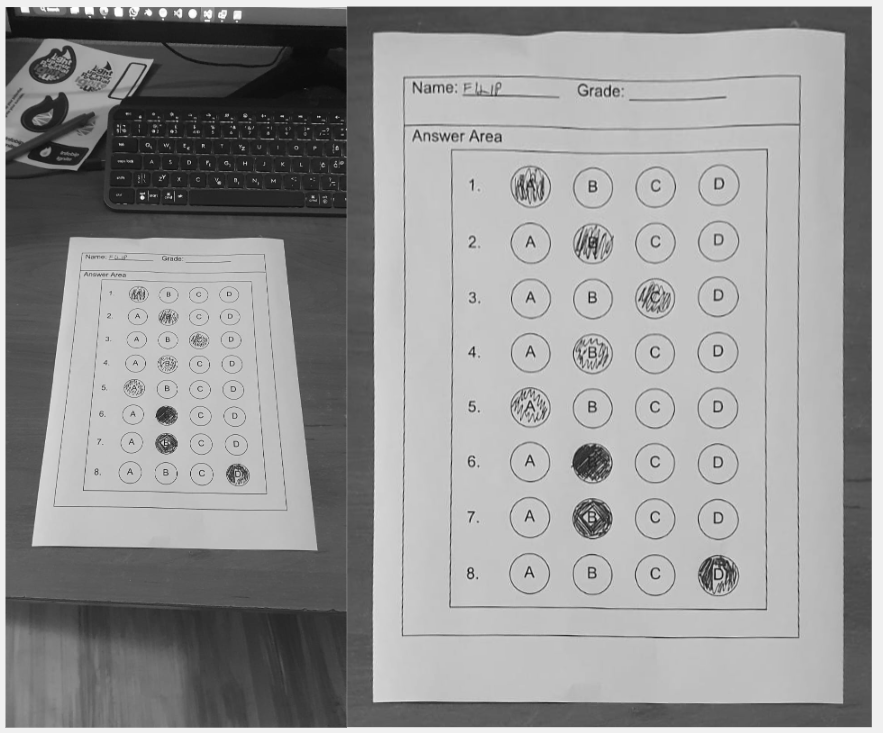
\includegraphics[width=0.8\linewidth]{slike/PerspectiveComparison.png}
\caption{Prikaz ulazne i izlazne slike CorrectPerspective metode (vlastita izrada)}
\end{figure}

Jedna od zanimljivosti ovog pristupa je to što se jako jednostavno može podržati ispravak perspektive slike na kojoj se ne nalazi cijeli papir. U tom slučaju pokušat će se i dalje pronaći najveći pravokutnik željenih proporcija, što u praksi znači da će se jedan od unutarnjih okvira sa slike uzeti u obzir. Time samo rješenje postaje još fleksibilnije.

Ispravak perspektive daje dobre rezultate, kao što je vidljivo na slici. Na slikama koje su također rotirane, rezultati su izrazito dobri jer ispravak perspektive ujedno ispravlja i rotaciju. No, u određenim slučajevima događa se da ispravak perspektive ne okrene papir pravilno, već je papir krivo orijentiran. Za takve situacije implementirana je sljedeća faza pretprocesiranja slike pomoću metode \texttt{CorrectRotation}:


\begin{lstlisting}[caption={Metoda za provjeru i ispravak orijentacije slike}]
override public ImageData CorrectRotation(ImageData inputImage){
    var inputMat = getMat(inputImage);
    var thresholded = ApplyThresholding(inputImage);
    RotatedRect nameRect = DetectNameRectangle(thresholded, inputMat);

    bool isUpsideDown = nameRect.Center.Y > inputMat.Height / 2;

    if (isUpsideDown){ inputMat = RotateImage(inputMat, 180); }

    return EmguCvImage.FromMat(inputMat, inputImage.Name);
}
\end{lstlisting}

\pagebreak
\begin{lstlisting}[caption={Metoda za rotaciju slike}]
private Mat RotateImage(Mat image, double angle){
    PointF center = new PointF(image.Width / 2, image.Height / 2);
    Mat rotationMatrix = new Mat();
    CvInvoke.GetRotationMatrix2D(center, angle, 1.0, rotationMatrix);

    Mat rotatedImage = new Mat();
    CvInvoke.WarpAffine(image, rotatedImage, rotationMatrix, image.Size, Inter.Linear, Warp.Default, BorderType.Constant, new MCvScalar(255, 255, 255));

    return rotatedImage;
}
\end{lstlisting}

Ova metoda bila je jedna od prvih razvijenih metoda; prva iteracija obuhvaćala je izračun kuta papira i ispravak tog kuta. No, s vremenom je metoda za ispravak perspektive preuzela dio tih odgovornosti, tako da je ova metoda sada isključivo odgovorna za detekciju orijentacije papira i rotaciju za 180 stupnjeva u slučaju da je papir u krivoj orijentaciji.

Kao što je već spomenuto, predložak matrice odgovora ne sadrži posebne oznake za kutove i orijentaciju papira. Zbog toga je bilo potrebno pronaći druge referentne strukture na predlošku. Odlučeno je koristiti okvir u kojem se nalaze polja za ime i ocjenu polaznika. Taj okvir nalazi se pri vrhu papira, stoga u slučaju da ga se detektira na dnu, znamo da je slika naopako okrenuta te ju se rotira za 180 stupnjeva pomoću metode \texttt{RotateImage}.

Ta je metoda bazirana na izračunu matrice rotacije koja se zatim primjenjuje na originalnu sliku. Matrica se izračunava pomoću metode \texttt{CvInvoke.GetRotationMatrix2D} i primjenjuje pomoću metode \texttt{CvInvoke.WarpAffine}.

\begin{figure}[H]
\centering
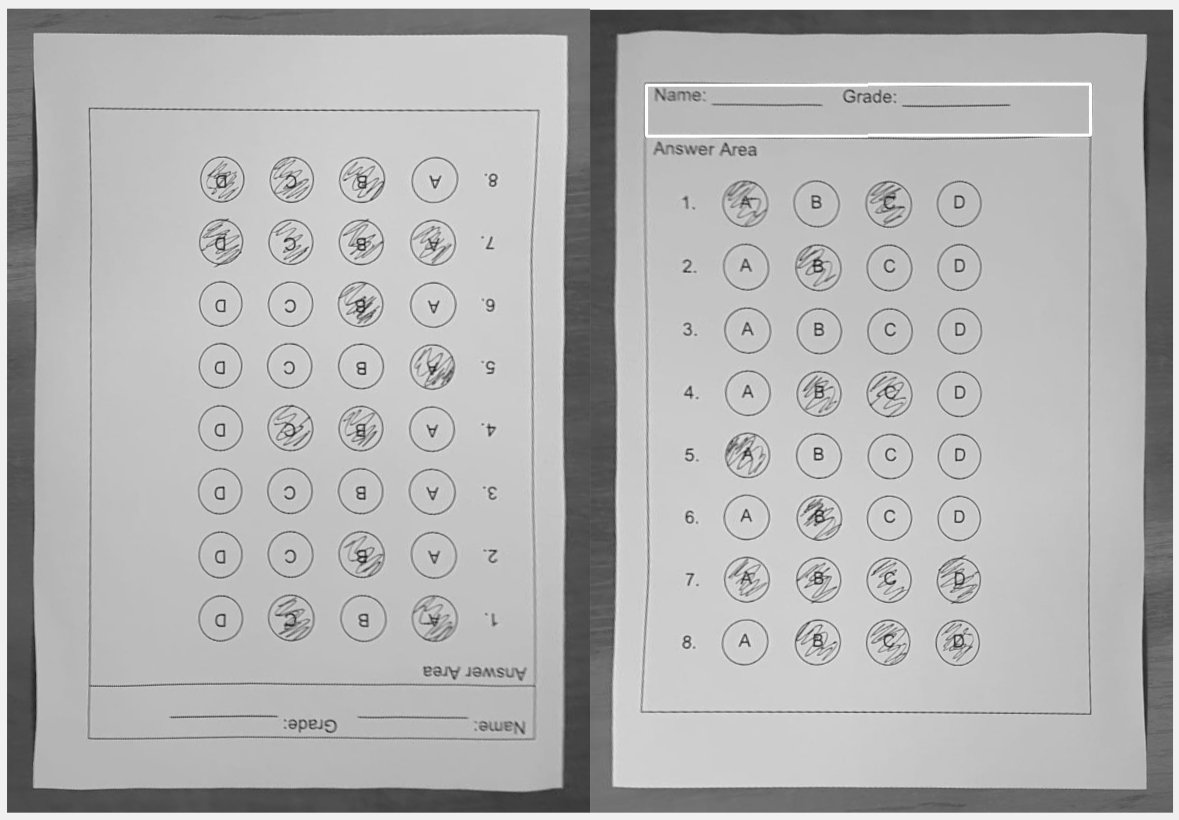
\includegraphics[width=0.7\linewidth]{slike/RotationComparison.png}
\caption{Prikaz ulazne i izlazne slike CorrectRotation metode (vlastita izrada)}
\end{figure}

Sa priložene slike vidljiv je rad \texttt{CorrectRotation} metode. S lijeve strane je ulazna slika s ispravljenom perspektivom, ali s krivom orijentacijom. S desne strane je rezultat metode koji prikazuje detektirani okvir za ime i ocjene te sliku nakon ispravka orijentacije.

Nakon provođenja svih dosad spomenutih operacija, rezultat je siva slika ispravne perspektive i orijentacije, sa smanjenom razinom buke. Prije nego što je moguće krenuti u analizu struktura radi pronalaska krugova, potrebno je ukloniti ostatak nepotrebnih informacija, poput nijansi sive boje. Upravo zbog toga proces izrade binarne slike provodi se pomoću metode \texttt{ApplyThresholding}:

\begin{lstlisting}[caption={Metoda za pretvorbu sive slike u binarnu sliku}]
override public ImageData ApplyThresholding(ImageData inputImage){
    var inputMat = getMat(inputImage);
    Mat threshMat = new Mat();
    CvInvoke.AdaptiveThreshold(inputMat, threshMat, 255, AdaptiveThresholdType.GaussianC, ThresholdType.BinaryInv, 11, 2);
    return EmguCvImage.FromMat(threshMat, inputImage.Name);
}
\end{lstlisting}

Priložena metoda poprilično je jednostavna i bazirana na metodi \texttt{CvInvoke.AdaptiveThreshold}, koja omogućuje bolje rezultate u varirajućim uvjetima osvjetljenja u usporedbi s klasičnom metodom \texttt{CvInvoke.Threshold}. Ovaj dio rada konstantno se mijenjao i kalibrirao tijekom razvoja. Na početku se koristila metoda \texttt{CvInvoke.Threshold}, što se pokazalo nedovoljnim kada je testni skup podataka proširen slikama koje sadrže sjene i slično. U tom trenutku počela se koristiti adaptivna verzija te metode. Osim toga, testirani su različiti algoritmi te metode, a na kraju je odabran GaussianC algoritam zbog manje količine buke u usporedbi s ostalim ponuđenim algoritmima.

\begin{figure}[H]
\centering
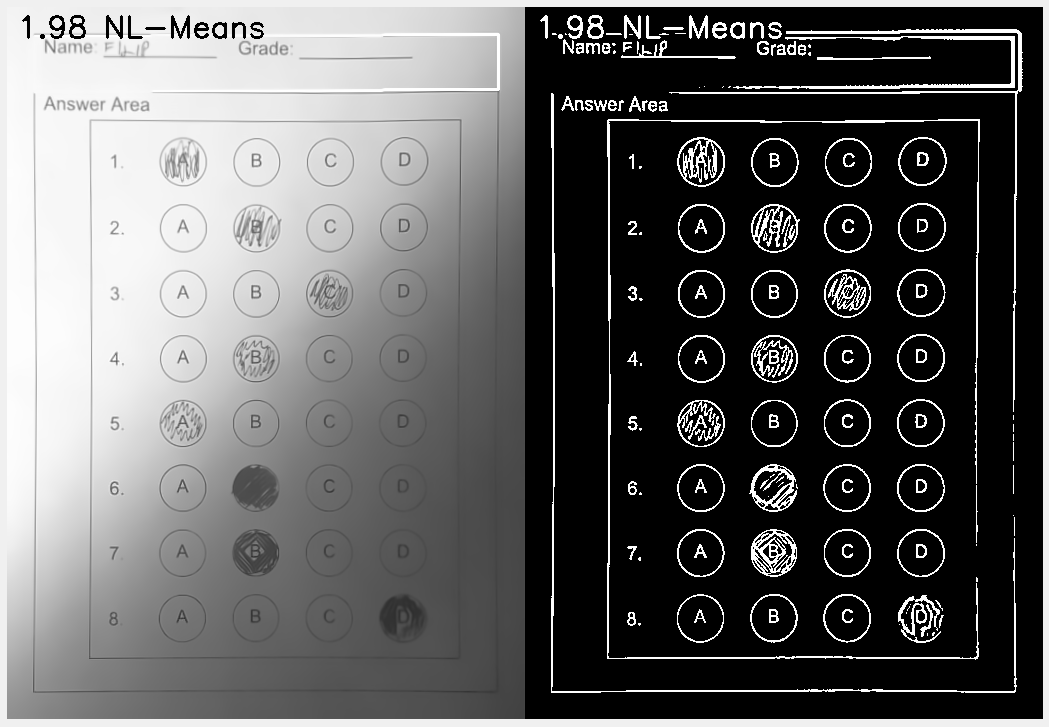
\includegraphics[width=0.7\linewidth]{slike/TresholdingComparison.png}
\caption{Prikaz ulazne i izlazne slike ApplyThresholding metode (vlastita izrada)}
\end{figure}

\pagebreak
Na lijevoj slici vidljivo je da je gornji dio slike jače osvijetljen naspram donjeg dijela slike, no na desnoj slici vidljivo je da je metoda uspjela izraditi ujednačenu binarnu sliku unatoč lošim uvjetima.

Time završava faza pretprocesiranja slike, što znači da je slika spremna za detektiranje strukturnih elemenata i njihovu analizu. Za taj dio odgovorna je metoda \texttt{CircleDetection}. Radi se o metodi koja zajedno s metodom za ispravak perspektive čini najkompleksniji dio sustava. Iz tog razloga primjeri prikazuju samo najznačajnije dijelove koda.

\begin{lstlisting}[caption={Metoda za detektiranje odgovora na slici}]
override public (ImageData, Dictionary<int, List<DetectedCircleBase>>) CircleDetection(ImageData input){
    var inputMat = getMat(input);
    var outputMat = new EmguCvImage().ToMat();
    //for debug
    CvInvoke.CvtColor(inputMat, outputMat, ColorConversion.Gray2Bgr);
    var allCircles = DetectAllCircles(inputMat, outputMat);
    var sortedCircleGroups = GroupAndSortCirclesByYPosition(allCircles);
    var random = new Random();
    DrawGroupedCircles(sortedCircleGroups, outputMat, random);
    var filteredGroups = FilterInvalidGroups(sortedCircleGroups, outputMat);
    var fillPercentages = filteredGroups.SelectMany(group => group.Value)
                                        .Select(c => GetFillPercentage(inputMat, (EmguCVCircle)c))
                                        .ToList();
    var threshold = HistogramGenerator.CalculateFillPercentageTreshold(fillPercentages);
    GenerateAndSaveFillPercentageHistogramIfNeeded(input, fillPercentages, threshold);
    DrawFilteredAndMarkGroups(filteredGroups, random, inputMat, threshold, outputMat);
    return (EmguCvImage.FromMat(outputMat, input.Name), filteredGroups);
}
\end{lstlisting}

Kroz kod može se vidjeti da je metoda \texttt{CircleDetection} odgovorna za:
\begin{enumerate}
    \item Detekciju svih krugova pomoću metode \texttt{DetectAllCircles}
    \item Grupiranje i sortiranje krugova po pitanjima pomoću metode \texttt{GroupAndSortCirclesByYPosition}
    \item Uklanjanje neispravnih krugova i grupa krugova pomoću metode \texttt{FilterInvalidGroups}
    \item Izračun praga za označenost pitanja pomoću klase \texttt{HistogramGenerator} i metode \texttt{CalculateFillPercentageThreshold}   
\end{enumerate}

Osim navedenih odgovornosti, ova metoda odgovorna je i za vizualizaciju svih koraka koje obavlja, no taj dio koda nema prevelik značaj.

Prva odgovornost ove metode je detekcija svih krugova pomoću metode:

\begin{lstlisting}[caption={Metoda za detektciju svih krugova na slici}]
private List<DetectedCircleBase> DetectAllCircles(Mat grayMat, Mat outputImage){
    VectorOfVectorOfPoint contours = new VectorOfVectorOfPoint();
    CvInvoke.FindContours(grayMat, contours, null, RetrType.List, ChainApproxMethod.ChainApproxSimple);
    var rawCircles = new List<DetectedCircleBase>();
    foreach (var contour in contours.ToArrayOfArray()){
        using (VectorOfPoint contourPoints = new VectorOfPoint(contour))
        {
            if (contourPoints.Size >= 20){
                RotatedRect ellipse = CvInvoke.FitEllipse(contourPoints);
                var circle = new CircleF(ellipse.Center, (float)(ellipse.Size.Width / 2));
                if (circle.Radius > MIN_CIRCLE_RADIUS && circle.Radius < MAX_CIRCLE_RADIUS){
                    rawCircles.Add(EmguCVCircle.FromCircleF(circle));
                }
            }
        }
    }
    var nonDuplicateCircles = FilterDuplicateCircles(rawCircles);
    return GetOnlyNonNestedCircles(nonDuplicateCircles, outputImage);
}
\end{lstlisting}

Detekcija krugova vrši se pronalaskom kontura pomoću metode \texttt{CvInvoke.FindContours}, a zatim pronalaskom kontura koje odgovaraju krugovima pomoću metode \texttt{CvInvoke.FitEllipse}. Osim same detekcije krugova, ova metoda obavlja i validaciju krugova te naknadno filtriranje. Validacije se odnose na provjeru broja točaka od kojih se kontura sastoji. Što više točaka kontura ima, to je vjerojatnije da je ta kontura relevantna. Ako je kontura relevantan krug, provjerava se je li taj krug unutar očekivanog raspona što se tiče radijusa. Ako jest, onda se dodaje u listu koja se zatim filtrira tako da se uklanjaju duplikati, to jest slični krugovi koji se preklapaju. Nakon toga lista krugova još se filtrira tako da se iz nje uklone svi krugovi koji se nalaze unutar drugih krugova.


\pagebreak
Nakon prve faze filtriranja i validacije krugova kreće grupiranje krugova po y koordinati, što zapravo znači da krugovi pripadaju istom pitanju. Zatim slijedi druga faza filtriranja, kojoj je cilj uklanjanje svih pitanja i krugova koji nisu valjani. Sljedeći kod prikazuje tu metodu:


\begin{lstlisting}[caption={Metoda za filtriranje neispravnih krugova i pitanja}]
private Dictionary<int, List<DetectedCircleBase>> FilterInvalidGroups(Dictionary<int, List<DetectedCircleBase>> sortedGroups, Mat outputImage){
    var validGroups = new Dictionary<int, List<DetectedCircleBase>>();
    foreach (var group in sortedGroups){
        var circles = group.Value;
        var sortedCircles = SortCirclesByXPosition(circles);
        var nonNestedCircles = GetOnlyNonNestedCircles(sortedCircles, outputImage, sortedCircles.Average(it => it.Y));
        var uniformCircles = GetCirclesWithUniformRadius(nonNestedCircles);
        if (isCircleGroupValid(uniformCircles, outputImage))
            validGroups.Add(group.Key, uniformCircles);
    }
    return validGroups;
}
\end{lstlisting}

Prije same validacije, krugovi se za svako pitanje sortiraju po x koordinati, što osigurava ispravan redoslijed odgovora. Zatim se dohvaćaju samo krugovi koji se ne nalaze unutar drugih krugova. Tim krugovima dodatno se validira jednakost radijusa i validnost grupe, to jest validnost razmaka između odgovora. Ovo je jedna od najvažnijih metoda, budući da uklanja nerelevantne i neispravno detektirane krugove. Rezultat ove metode je lista ispravnih krugova grupiranih po pitanjima. Zatim slijedi izračun praga ispunjenosti kruga pomoću metode \texttt{}:



\begin{lstlisting}[caption={Metoda za izračun postotka ispunjenosti kruga}]
private double GetFillPercentage(Mat thresholdedImage, EmguCVCircle circle){
    using (Mat mask = new Mat(thresholdedImage.Size, DepthType.Cv8U, 1))    {
        mask.SetTo(new MCvScalar(0));
        DrawCircle(mask, circle, new MCvScalar(255), -1);
        MCvScalar mean = CvInvoke.Mean(thresholdedImage, mask);
        return (mean.V0 / 255.0) * 100;
    }
}
\end{lstlisting}

Ova metoda izračunava postotak ispunjenosti tako da uspoređuje prosječnu vrijednost piksela unutar originalnog kruga s vrijednostima unutar binariziranog (crnog) kruga. Rezultat se vraća kao postotak ispunjenosti.
\pagebreak
No, da bi se moglo zaključiti je li krug ispunjen ili ne, potrebno je dobivenu vrijednost usporediti s pragom ispunjenosti koji je izračunat pomoću klase \texttt{HistogramGenerator} i metode \texttt{CalculateFillPercentageThreshold}:

\begin{lstlisting}[caption={Metoda za filtriranje neispravnih krugova i pitanja}]
public static double CalculateFillPercentageTreshold(List<double> fillPercentages){
    var histogram = new List<int>(new int[101]);
    fillPercentages.ForEach(fill => histogram[(int)Math.Floor(fill)]++);
    var startOfFirstPeak = histogram.FindIndex(x => x > 0);
    var endOfFirstPeak = histogram.Skip(startOfFirstPeak + 1).ToList().FindIndex(x => x == 0) + startOfFirstPeak + 1;
    while (endOfFirstPeak + 2 < histogram.Count &&
            (histogram[endOfFirstPeak + 1] > 0 || histogram[endOfFirstPeak + 2] > 0)){
        endOfFirstPeak++;
    }
    return endOfFirstPeak;
}
\end{lstlisting}

Priložena metoda računa prag ispunjenosti kruga. Na početku razvoja definirana je konstanta koja je predstavljala taj prag, no taj pristup se kroz razvoj pokazao nedovoljnim. Problem je u tome što matrice odgovora mogu imati različit broj pitanja i odgovora, što znači da postotak ispunjenosti kruga značajno varira o veličini kruga na predlošku. Osim toga, postotak ispunjenosti također ovisi o načinu na koji se matrica ispunjava.

Zbog toga definiranje praga pomoću konstante više nije bilo adekvatno rješenje. U tom trenutku bilo je jasno da je potrebno izračunati prag ispunjenosti, no rješenje nije bilo jasno. Zbog toga je generirana sljedeća slika koja je pružila uvid u podatke o ispunjenosti svih krugova na slici.

\begin{figure}[H]
\centering
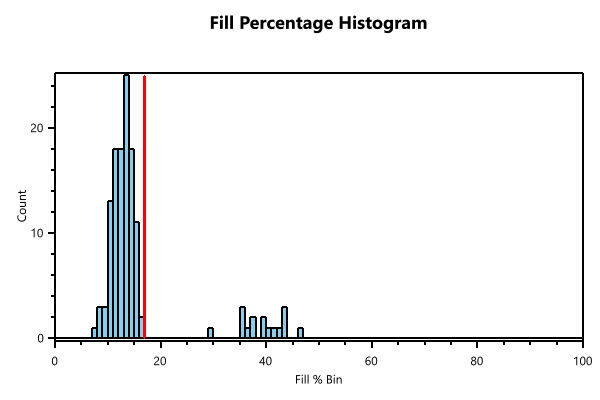
\includegraphics[width=0.7\linewidth]{slike/histogram.png}
\caption{Prikaz histograma postataka ispunjesnosti krugova (vlastita izrada)}
\end{figure}
\pagebreak
Sa priložene slike bilo je jasno da postoje dva jasno definirana i odvojena dijela grafa. Prvi dio podataka prikazuje postotak ispunjenost za prazne krugove, dok drugi dio prikazuje postotak ispunjenosti za ispunjene krugove. Važno je napomenuti i da prazni krugovi imaju određeni postotak ispunjenosti zbog oznaka odgovora koje mogu biti od slova A do H.

Nakon analize histograma bilo je jasno da je prag ispunjenosti kraj prvog seta podataka na grafu. Točno to se vidi u metodi \texttt{CalculateFillPercentageThreshold}. Pronalazi se početak prvog seta podataka, a zatim prvo točka koja nakon sebe ima barem dva prazna postotna boda, što znači da je zapravo to ispravna granica. Ovo rješenje automatski rješava jedan od tradicionalnih problema OMR sustava, gdje korisnici ne prate upute za ispunjavanje odgovora.

Prikazane metode zajedno omogućuju detekciju odgovora i pitanja prikazanu na priloženoj slici.

\begin{figure}[H]
\centering
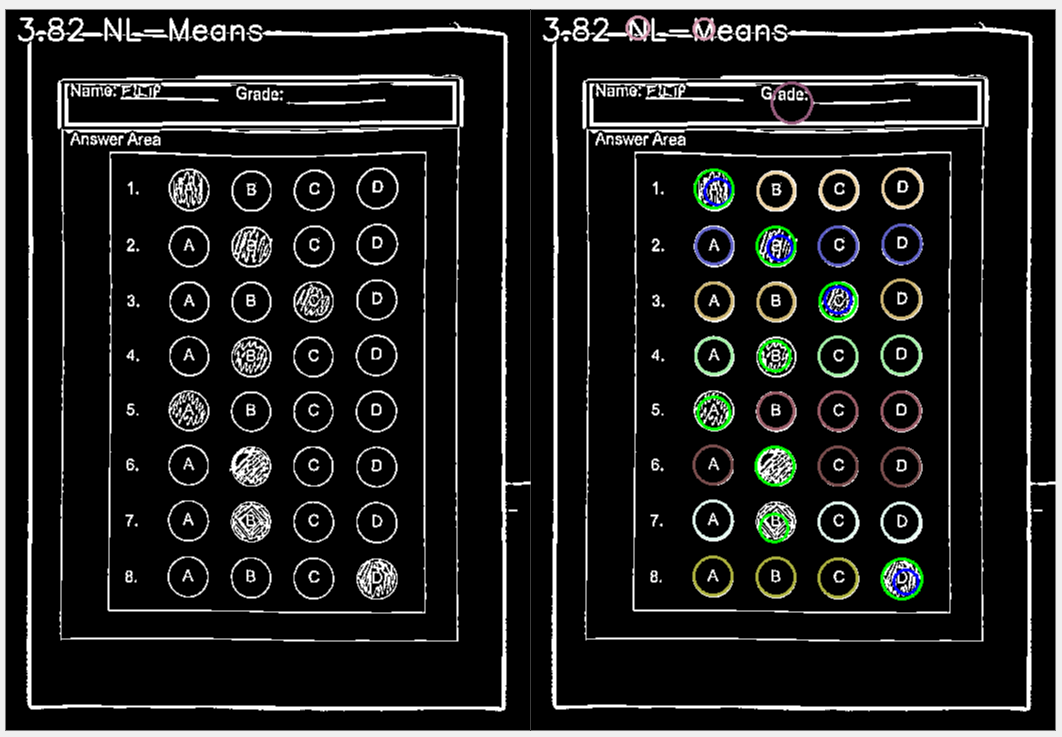
\includegraphics[width=0.8\linewidth]{slike/CircleDetectionComp.png}
\caption{Prikaz ulazne i izlazne slike CircleDetection metode (vlastita izrada)}
\end{figure}

Lijeva slika prikazuje ulazne podatke metode \texttt{CircleDetection}, dok desna slika prikazuje dio izlaznih podataka te metode. Na desnoj slici vidljivi su krugovi u raznim bojama, gdje svaka boja označava grupu pitanja. Važno je napomenuti da ta slika sadrži i nevažeće krugove koji su bili uklonjeni. Ta slika sadrži sve te podatke radi lakšeg pronalaska grešaka. Do sada su svim metodama za obradu slike glavni rezultati također bile slike, no ovdje je glavni rezultat lista validnih odgovora grupiranih i sortiranih po pitanjima.

Ostale metode obrade slike nisu prikazane kroz kod jer ne sadrže zanimljivu ni značajnu logiku. Većinom se radi o metodama za vizualizaciju rezultata ocjenjivanja i klasama za ocjenjivanje koje su bazirane na usporedbi lista odgovora.

\chapter{Evaluacija}

Kroz ovo poglavlje fokus će biti na prikazu načina evaluacije razvijenih artefakata. Pod to spada prikaz različitih tipova testnih podataka, koraka obrade i načina manuelnog testiranja artefakata. Također će se objasniti utjecaj testiranja i testnih podataka na razvoj artefakata.

\section{Skup testnih podataka}

Testni podaci uključuju razne tipove matrica odgovora. Matrice sadrže različit broj pitanja i odgovora što omogućuje verifikaciju funkcionalnosti detektiranja odgovora na različitim konfiguracijama. Osim različitih konfiguracija, testni podaci također sadrže slike s različitim pozadinama iza papira, udaljenostima kamere od papira, uvjetima osvjetljenja i slično. Na priloženoj slici vidljivi su različiti tipovi matrica odgovora korištenih za testiranje.

\begin{figure}[H]
\centering
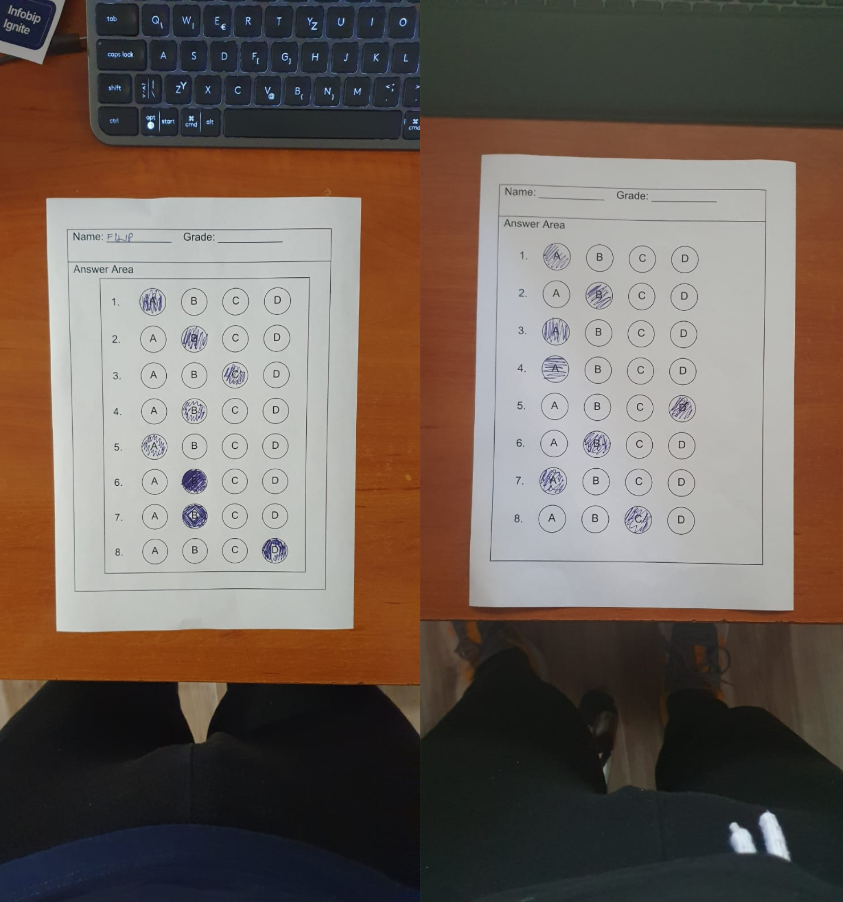
\includegraphics[width=0.8\linewidth]{slike/Test1.png}
\caption{Prikaz različitih tipova matrica odgovora - primjer 1 (vlastita izrada)}
\end{figure}

\begin{figure}[H]
\centering
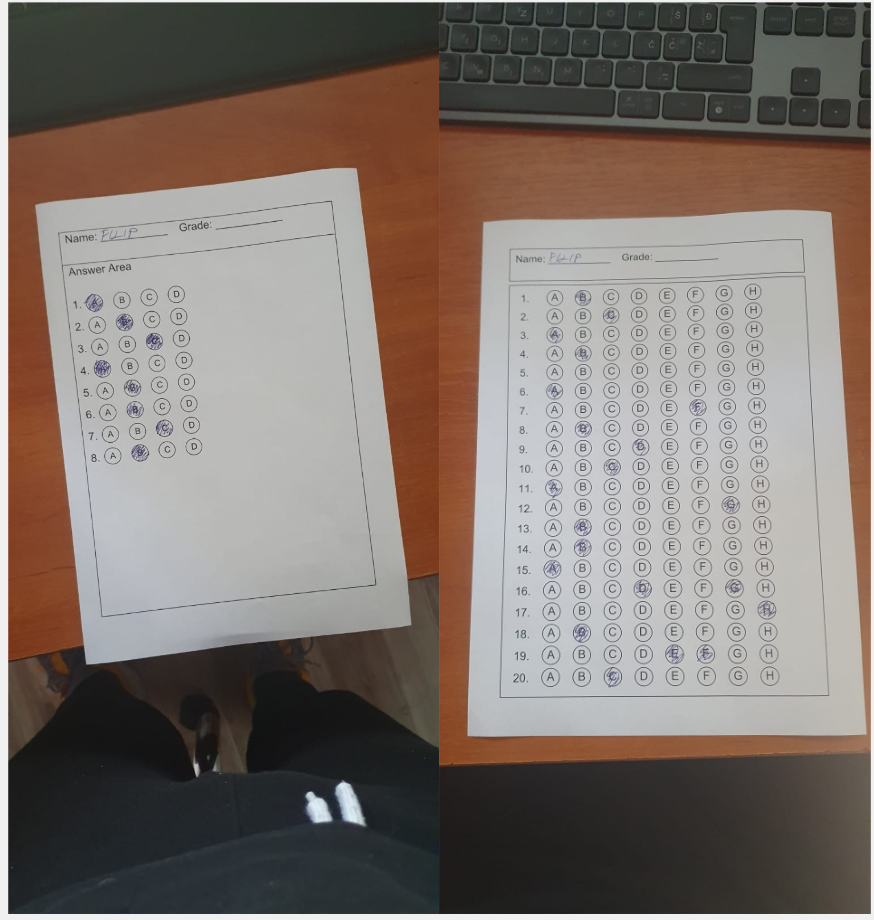
\includegraphics[width=0.8\linewidth]{slike/Test2.png}
\caption{Prikaz različitih tipova matrica odgovora - primjer 2 (vlastita izrada)}
\end{figure}

Sa priloženih slika vidljivo je da postoji razlika u broju pitanja i odgovora po pitanju, veličini krugova za odgovore te u samoj strukturi matrice odgovora. Lijeva slika na slici 30 prikazuje jedan od prvih izrađenih predložaka. Sastojao se od okvira za ime i ocjenu polaznika, okvira za područje odgovora te još jednog dodatnog okvira unutar tog okvira. Ti su okviri na početku testiranja služili da sustavu daju priliku za detekciju okvira u slučaju da rub papira nije uspješno detektiran. Tijekom razvoja, ti su okviri postali sve manje važni za funkcioniranje sustava, pa je unutarnji okvir uklonjen. Ostali okviri su ostali jer služe kao pomoć sustavu kada slika ne sadrži sva tri kuta papira, tada se koristi okvir kao alternativa.

Osim toga, moguće je primijetiti da je okvir za ime na desnoj slici (slika 31) odvojen od glavnog okvira za pitanja. To je jedna od zadnjih promjena na predlošku. Cilj te promjene bio je provjeriti hoće li se preciznost detekcije okvira za ime poboljšati ako su okviri odvojeni. Kroz testiranje je zaključeno da jest, te da je preciznost porasla.

Osim strukturnih elemenata, na slikama se mogu vidjeti različiti kutovi i nagibi kamere u odnosu na papir, kao i pozadinski elementi poput tipkovnice. Slike su snimljene na takav način da se provjere mogućnosti sustava. Ovi primjeri prikazuju uvjete korištenja koje sustav može u većini slučajeva bez problema podnijeti.

Na sljedećim primjerima prikazane su slike snimljene u zahtjevnijim uvjetima:

\begin{figure}[H]
\centering
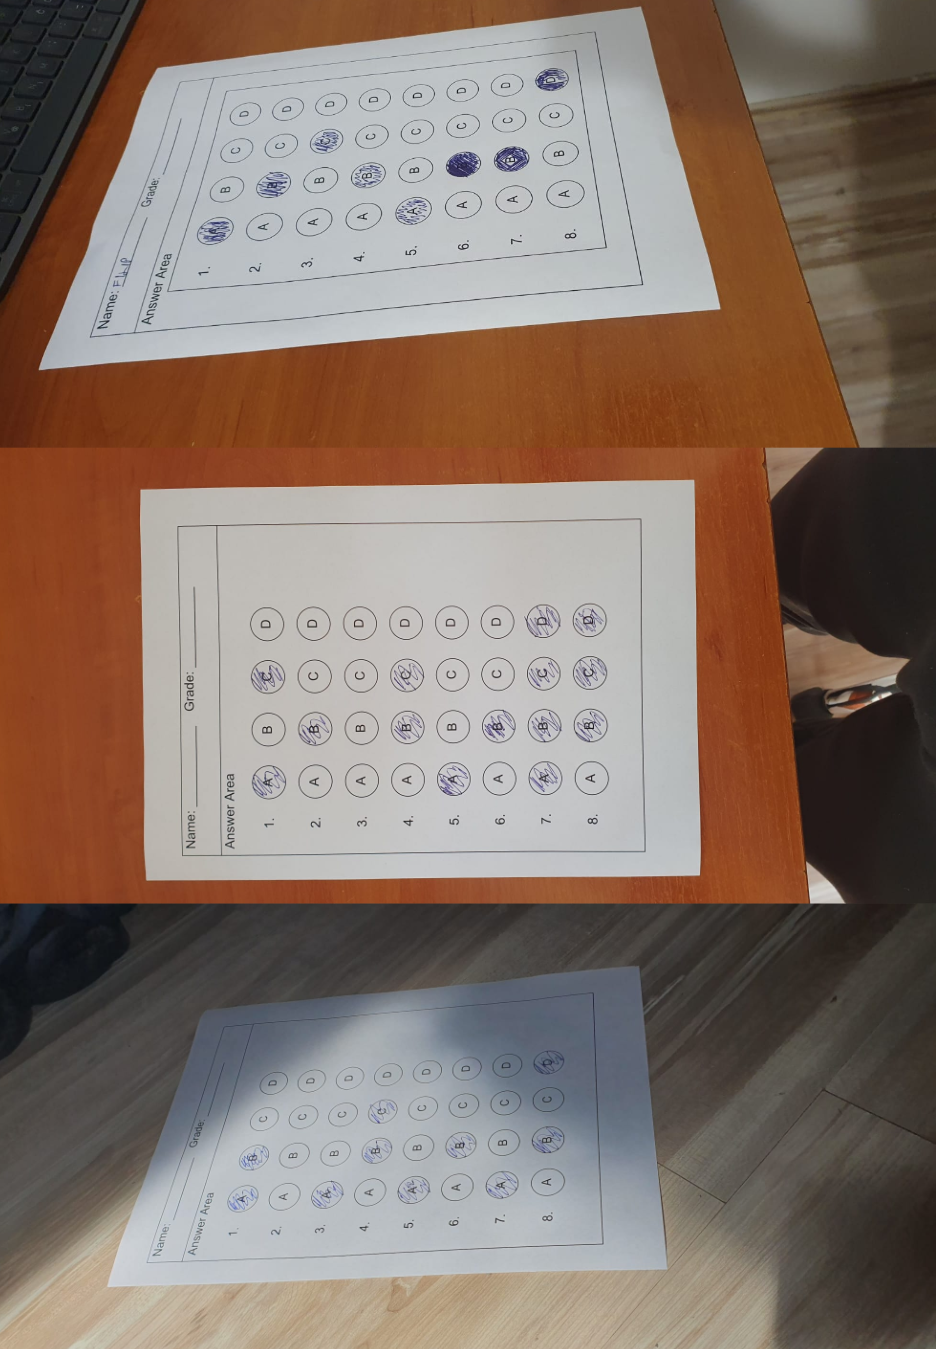
\includegraphics[width=0.5\linewidth]{slike/Test3.png}
\caption{Prikaz matrica odgovora uslikanim u izazovnijim uvjetima - primjer 1 (vlastita izrada)}
\end{figure}

\begin{figure}[H]
\centering
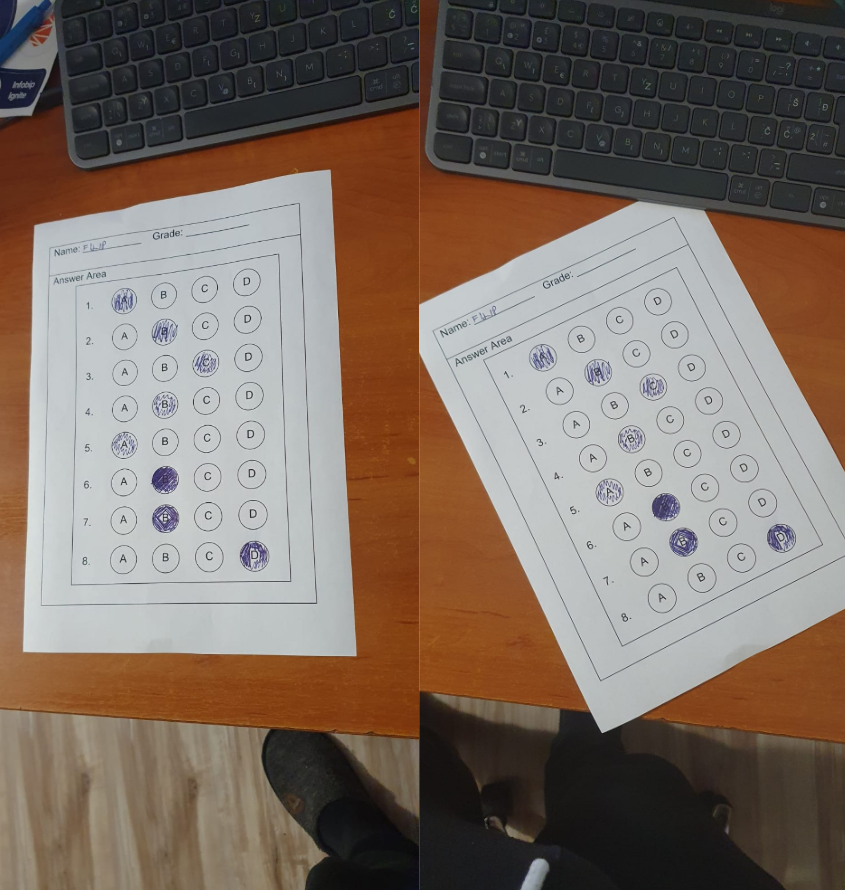
\includegraphics[width=0.55\linewidth]{slike/Test4.png}
\caption{Prikaz matrica odgovora uslikanim u izazovnijim uvjetima - primjer 2 (vlastita izrada)}
\end{figure}

Radi se o slikama snimljenim s krivim orijentacijama papira, ekstremnim perspektivama i nepovoljnim uvjetima osvjetljenja. Na nekim slikama također nedostaju kutovi papira. Takvi uvjeti nisu idealni za rad sustava, ali upravo zahvaljujući njima sustav je testiran i poboljšan kako bi mogao raditi preciznije čak i u ekstremnim situacijama. Sustav je dizajniran da vizualizira rezultate ocjenjivanja te da javi grešku ukoliko ne može ispravno obraditi sliku. Time se ocjenjivačima omogućuje da provjere rezultate ocjenjivanja, budući da su oni ipak odgovorne osobe u cijelom procesu.

\subsection{Prikaz koraka obrada slike nad testnim podatcima}

Kroz ovo poglavlje prikazat će se ukratko svi koraci kroz koje slika prolazi prije nego što se rezultat ocjenjivanja prikaže na ekranu ocjenjivača. Koraci su vrlo slični koracima prikazani u analizi koda no redosljed operacija se malo promjenio kroz razvoj artefakta.

\begin{figure}[H]
\centering
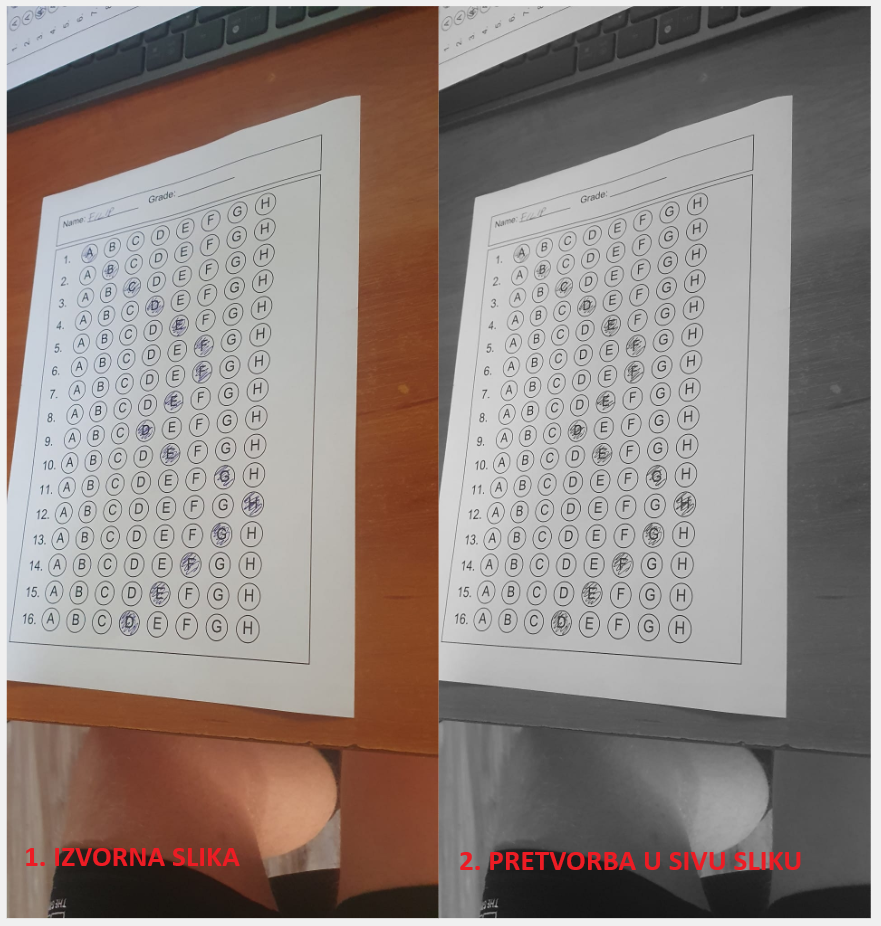
\includegraphics[width=0.85\linewidth]{slike/null (7).png}
\caption{Prikaz izvorne slike i pretvorbe u sivu sliku na primjeru (vlastita izrada)}
\end{figure}

\begin{figure}[H]
\centering
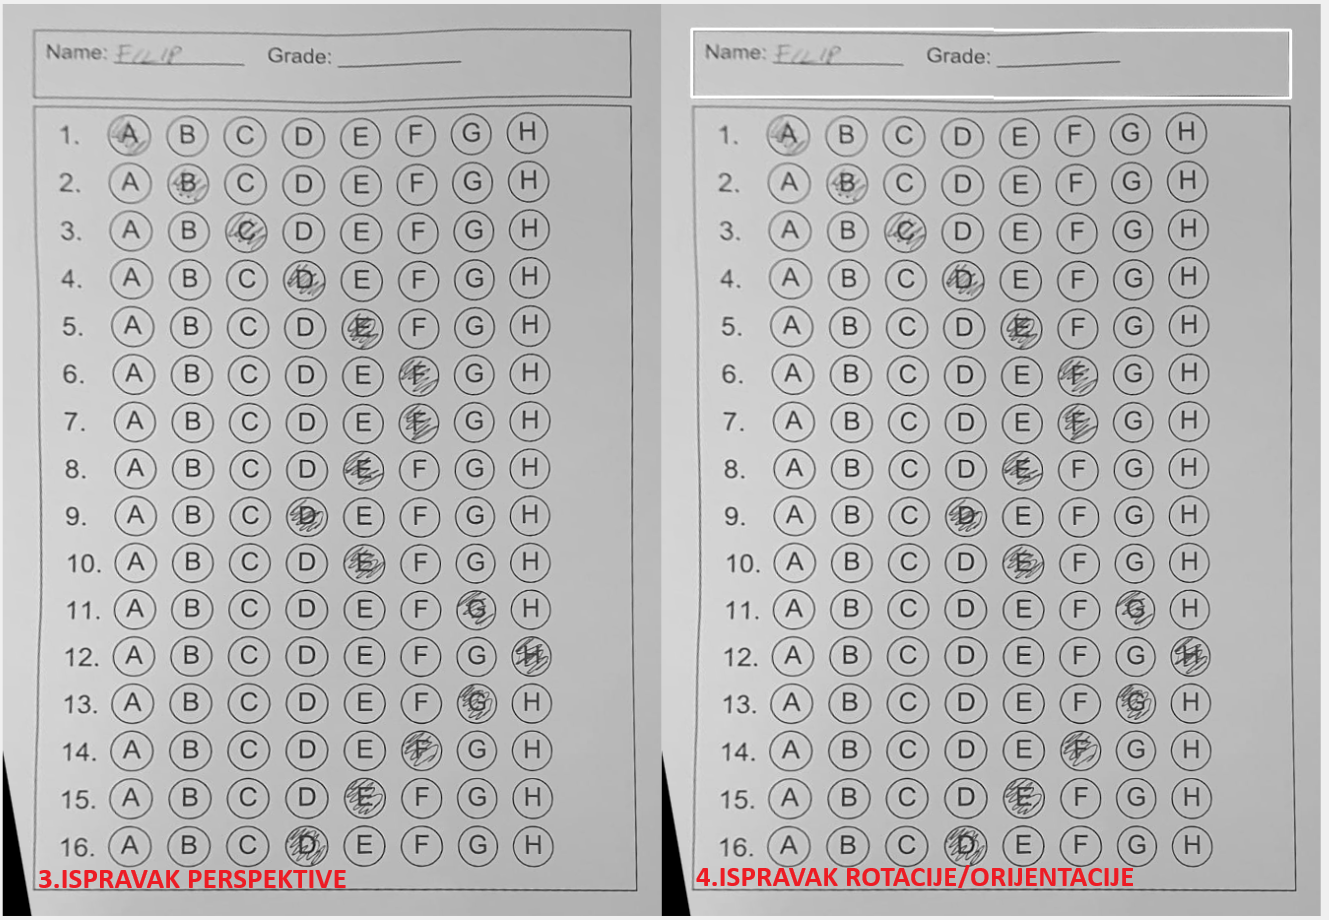
\includegraphics[width=0.85\linewidth]{slike/null (8).png}
\caption{Prikaz ispravka perspektive i rotacije na primjeru (vlastita izrada)}
\end{figure}

\begin{figure}[H]
\centering
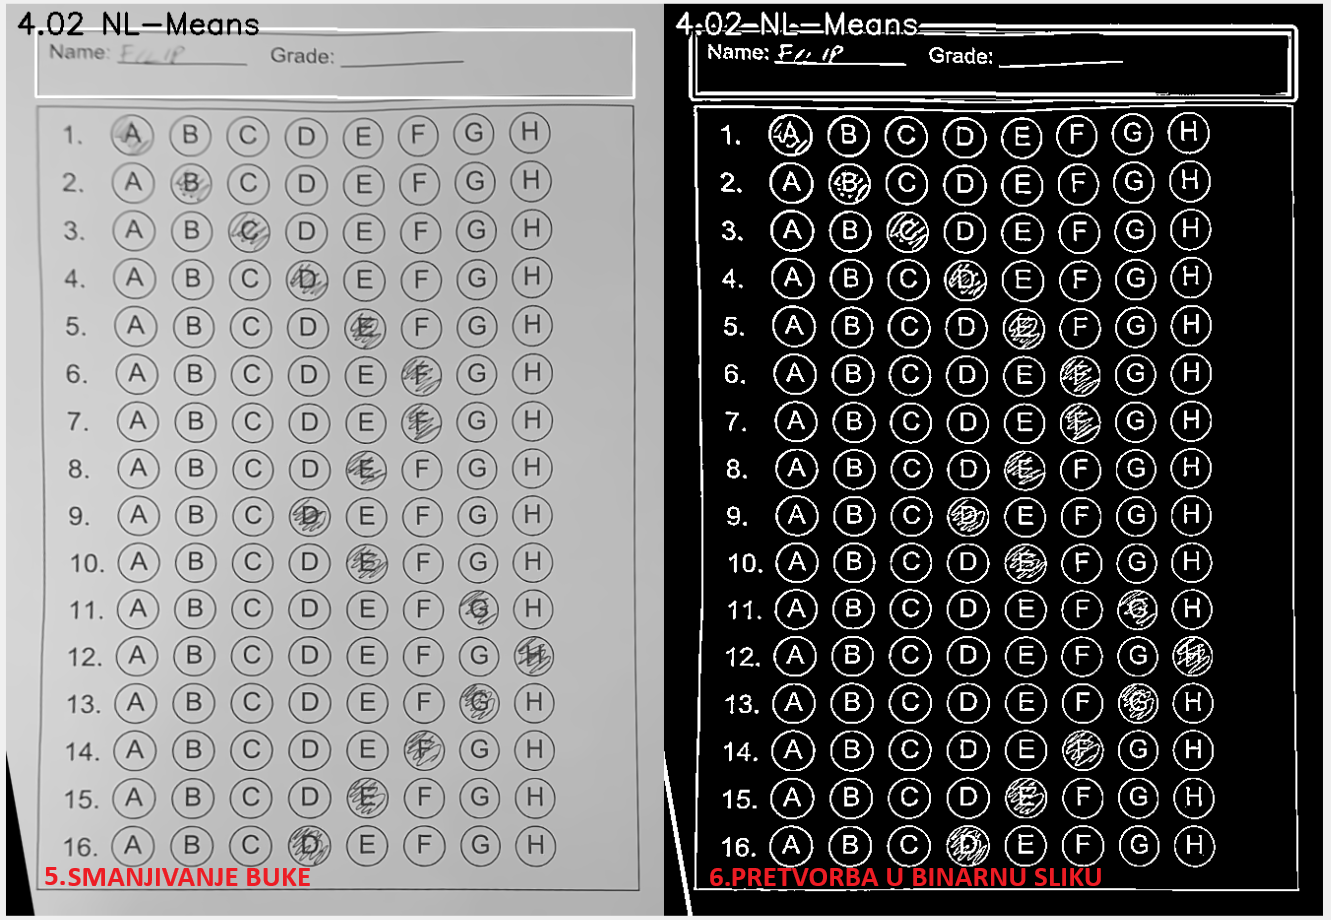
\includegraphics[width=0.85\linewidth]{slike/null (9).png}
\caption{Prikaz smanjivanja buke i pretvorbe u binarnu sliku na primjeru (vlastita izrada)}
\end{figure}

\begin{figure}[H]
\centering
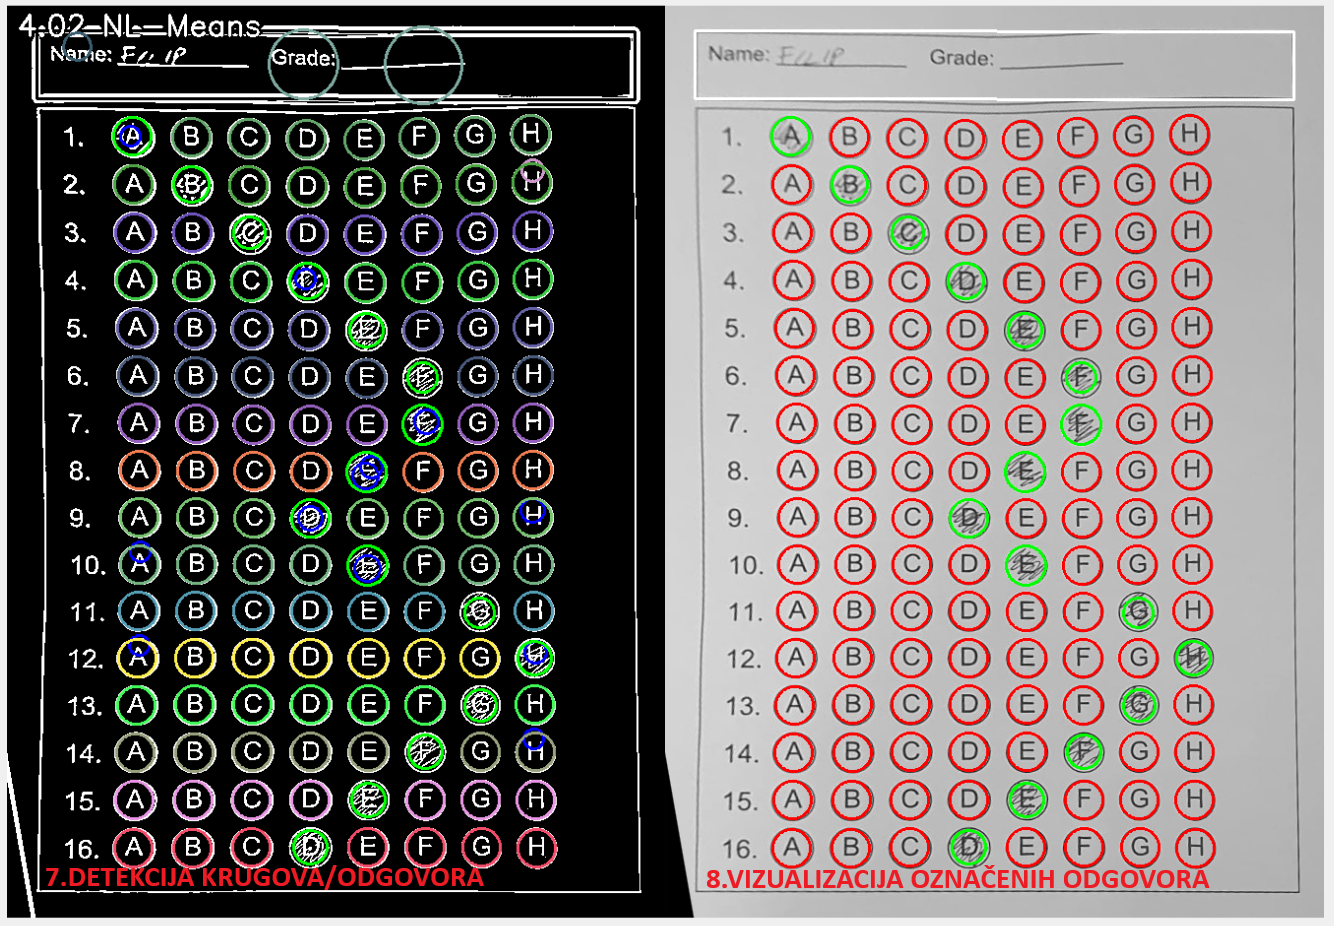
\includegraphics[width=0.8\linewidth]{slike/null (10).png}
\caption{Prikaz detekcije odgovora i vizualizacije označenih odgovora na primjeru (vlastita izrada)}
\end{figure}

\begin{figure}[H]
\centering
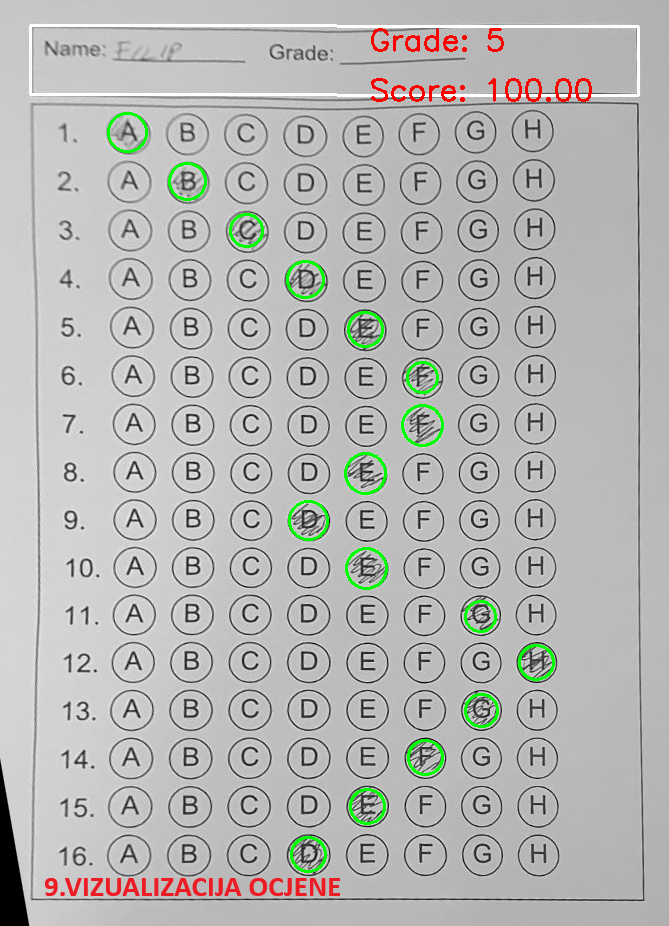
\includegraphics[width=0.55\linewidth]{slike/08_VisualizeGrade.png}
\caption{Prikaz vizualizacije ocjene na primjeru (vlastita izrada)}
\end{figure}

Sa priloženih slika vidljivi su koraci kroz koje je izvorna slika prošla da bi se mogla ocijeniti. Radi se o slici koja nije snimljena u idealnim uvjetima. Neki od problema vidljivih na slici su neispravna perspektiva, papir koji nije u potpunosti prikazan, blaga neujednačenost osvjetljenja, te prisutnost neželjenih elemenata poput tipkovnice u kadru. Unos slike u sustav predstavlja prvi korak obrade.

Od samog početka razvoja bilo je jasno da je drugi korak pretprocesiranja pretvorba slike u sivu skalu, odnosno uklanjanje boja. Testni podaci nisu značajno utjecali na ovu odluku, no imali su važnu ulogu u određivanju redoslijeda ostalih operacija u fazi pretprocesiranja.

Razvoj je započeo s uklanjanjem buke kao trećom operacijom, popraćenom ispravkom rotacije. Međutim, tijekom testiranja postalo je jasno da slike ne moraju imati samo krivu rotaciju papira, već i nagib kamere u odnosu na papir, odnosno perspektivnu distorziju. Dosadašnji pristup u takvim slučajevima nije bio dovoljan, pa je razvijen korak za ispravak perspektive. Daljnjim testiranjem zaključeno je da je preciznost sustava veća ako se smanjivanje buke postavi nakon ispravka perspektive i rotacije. Tako je dobiven sljedeći redoslijed koraka:

\begin{enumerate}
    \item Unos slike u sustav
    \item Pretvorba u sivu sliku
    \item Ispravak perspektive
    \item Ispravak rotacije
    \item Smanjivanje buke
\end{enumerate}

Taj redoslijed opisuje gotovo cijelu fazu pretprocesiranja slike, s tim da kao završni korak pretprocesiranja nedostaje još samo pretvorba u binarnu sliku. Taj korak omogućuje uklanjanje nepotrebnih informacija i fokusiranje na ključne strukture prisutne na slici. U binarnoj slici pozadina je prikazana crnom bojom, dok su sve relevantne strukture označene bijelom bojom.

Nakon završetka pretprocesiranja, slijedi faza procesiranja slike, gdje je prvi logičan korak detekcija krugova. Sama detekcija krugova relativno je jednostavna za implementirati, kao što je prikazano u priloženom kodu. Međutim, ključni dio ove faze je odvajanje relevantnih krugova od nerelevantnih te izračun praga ispunjenosti kruga. Upravo je ovaj segment sustava najviše unaprijeđen zahvaljujući raznovrsnom skupu testnih podataka.

Na slici 37 prikazana je vizualizacija svih koraka rada ove faze. Nakon detekcije ispunjenih krugova, slijede još dva koraka fokusirana na vizualizaciju rezultata.

Važno je istaknuti da su priložene slike generirane u načinu rada za otklanjanje grešaka te se spremaju u mapu na radnoj površini. Ova funkcionalnost omogućila je dubinski uvid u rad sustava tijekom razvoja i znatno ubrzala pronalazak i otklanjanje grešaka. Osim toga, može biti vrlo korisna i ocjenjivačima koji žele provjeriti gdje je ocjenjivanje određenog ispita eventualno pošlo po krivu. Ključna značajka ovog rješenja je da se svaka greška uvijek može reproducirati jer će isti ulazni podatak uvijek rezultirati istim izlazom.

\section{Manualno testiranje rješenja}

\begin{table}[H]
\centering
\begin{tabular}{|l|p{11cm}|}
\hline
\textbf{Identifikator} & TS-01 \\ \hline
\textbf{Naziv scenarija} & Detekcija odgovora na matrici \\ \hline
\textbf{Cilj} & Provjeriti ispravnost detekcije odgovora s učitane slike matrice odgovora. \\ \hline
\textbf{Ulaz} & Slika ispunjene matrice odgovora s različitim vrstama označenih odgovora (označeni, prazni, djelomično označeni). \\ \hline
\textbf{Očekivani ishod} & 
\begin{itemize}
    \item Sustav točno identificira pozicije svih odgovora.
    \item Klasificira ih kao označene ili prazne.
    \item Pridružuje ih ispravnom pitanju.
\end{itemize} \\ \hline
\multicolumn{2}{|c|}{} \\ \hline

\textbf{Identifikator} & TS-02 \\ \hline
\textbf{Naziv scenarija} & Usporedba odgovora i dodjela ocjene \\ \hline
\textbf{Cilj} & Testirati ispravnost usporedbe odgovora i dodjele ocjene prema definiranoj skali. \\ \hline
\textbf{Ulaz} & Lista detektiranih odgovora na ispitu za ocjenjivanje, lista kontrolnih odgovora, definirana skala ocjenjivanja. \\ \hline
\textbf{Očekivani ishod} & 
\begin{itemize}
    \item Dodijeljena odgovarajuća ocjena prema definiranoj skali.
    \item Prikazana vizualna oznaka točnih i netočnih odgovora.
    \item Prikaz postotka točnosti ispita
\end{itemize} \\ \hline
\multicolumn{2}{|c|}{} \\ \hline

\textbf{Identifikator} & TS-03 \\ \hline
\textbf{Naziv scenarija} & Generiranje predloška \\ \hline
\textbf{Cilj} & Testirati generiranje PDF predloška. \\ \hline
\textbf{Ulaz} & Definirani broj pitanja i odgovora po pitanju. \\ \hline
\textbf{Očekivani ishod} & 
\begin{itemize}
    \item Predložak se ispravno generira i odgovara zadanim parametrima.
\end{itemize} \\ \hline
\end{tabular}
\caption{Scenariji za manualno testiranje}
\end{table}

Ovo su glavni scenariji prema kojima se testiralo rješenje tijekom razvoja. Upute za sve scenarije su iste i uključuju pokretanje sustava nad cijelim skupom testnih podataka te verifikaciju ishoda u sučelju ili analizu datoteka generiranih u načinu rada za otklanjanje grešaka.

\chapter{Diskusija}
\section{Analiza rezultata}
\section{Limitacije rješenja}
\section{Poboljšanja rješenja}

\chapter{Zaključak}

\printbibliography[title=Popis literature]
\addcontentsline{toc}{chapter}{Popis literature}

\listoffigures
\addcontentsline{toc}{chapter}{Popis slika}
 
\listoftables
\addcontentsline{toc}{chapter}{Popis popis tablica}

\appendix
\renewcommand{\thechapter}{\arabic{chapter}}


\end{document}